%MIT OpenCourseWare: https://ocw.mit.edu
%18.156 Projection Theory (Spring 2025)
%License: Creative Commons BY-NC-SA 
%For information about citing these materials or our Terms of Use, visit: https://ocw.mit.edu/terms.

\documentclass[12pt]{amsart}
\usepackage{geometry}                % See geometry.pdf to learn the layout options. There are lots.
\geometry{letterpaper}                   % ... or a4paper or a5paper or ... 
%\geometry{landscape}                % Activate for for rotated page geometry
%\usepackage[parfill]{parskip}    % Activate to begin paragraphs with an empty line rather than an indent
\usepackage{graphicx}
\usepackage{amssymb}
\usepackage{amsmath}
\usepackage{wrapfig}
\usepackage{tikz}
\usepackage{amsthm}
\usepackage{subcaption}
\usepackage[export]{adjustbox}
\usepackage{pgfplots}
\usetikzlibrary{calc}
\usetikzlibrary{patterns}

\definecolor{myblack}{RGB}{0,0,0}
\definecolor{mygray}{RGB}{230,230,230}
\definecolor{myblue}{RGB}{74,144,226}
\definecolor{myred}{RGB}{226,74,74}
\definecolor{mytan}{RGB}{225,185,127}
\definecolor{myyellow}{RGB}{244,255,48}
\definecolor{myorange}{RGB}{245,166,35}
\definecolor{mypink}{RGB}{229,144,144}
\definecolor{mygreen}{RGB}{0,128,0}
\definecolor{myolive}{RGB}{144,139,66}
\definecolor{myyellowgreen}{RGB}{148,171,12}

\newtheorem{theorem}{Theorem}[section]
\newtheorem{lemma}[theorem]{Lemma}
\newtheorem{conj}[theorem]{Conjecture}
\newtheorem{Example}[theorem]{Example}
\newtheorem{example}[theorem]{Example}
\newtheorem{remark}[theorem]{Remark}
\newtheorem{Definition}[theorem]{Definition}
\newtheorem{Corollary}[theorem]{Corollary}
\newtheorem{prop}[theorem]{Proposition}
\newtheorem{notation}[theorem]{Notation}
\newtheorem{corollary}[theorem]{Corollary}
\newtheorem{question}[theorem]{Question}
\DeclareMathOperator{\Hopf}{Hopf}
\DeclareMathOperator{\Dir}{Dir}

\newcommand{\F}{\mathbb{F}}
\newcommand{\FF}{\mathbb{F}}
\newcommand{\CC}{\mathbb{C}}
\newcommand{\del}{\partial}
\newcommand{\QQ}{\mathbb{Q}}
\newcommand{\ZZ}{\mathbb{Z}}
\newcommand{\RR}{\mathbb{R}}
\DeclareMathOperator{\HD}{HD}
\newcommand{\LL}{\mathbb{L}}
\newcommand{\spp}{\textrm{supp}}
\newtheorem{ques}{Question}
\newcommand{\T}{\mathbb{T}}
\newcommand{\TT}{\mathbb{T}}
\newcommand{\eps}{\epsilon}
\newcommand{\Z}{\mathbb{Z}}
\newcommand{\Gr}{\mathrm{Gr}}
\newcommand{\vol}{\mathrm{vol}}
\newcommand{\poly}{\mathrm{Poly}}


\begin{document}

\title{Projection theory notes}

\maketitle
\setcounter{tocdepth}{1}


Given a set or measure in Euclidean space,  we consider its projection onto many different subspaces.   Informally,  we study an object by looking at its shadows in many different directions.   How do the features of the object compare with the features of the shadows?  If many shadows are highly concentrated,  is the original object highly concentrated too?  This type of question connects geometry and harmonic analysis and combinatorics.   

Understanding this type of question has applications in number theory,  homogeneous dynamics  and harmonic analysis.  Some of these connections were just found recently.  Seeing all the connections between projection theory and other areas was one motivation to teach this class.

One of the fundamental problems in the subject is called the exceptional set problem.  It is a quantitative version of the question from the first paragraph:  If many shadows are highly concentrated,  is the original object highly concentrated too?  This question was introduced in the 1960s.  It was fully answered in 2024 by Orponen-Shmerkin-Ren-Wang.   This breakthrough was a second motivation to teach this class.

The full proof of Orponen-Shmerkin-Ren-Wang is quite complex,  and we won't study every detail,  but we will introduce the background and describe the main new ideas.

In the class, we will introduce projection theory,   learn some classical methods,  explore how it connects to other areas,  and study some recent developments.

\vskip10pt

{\bf Acknowledgements. } Thanks to Pablo Shmerkin,  who visited for a month during this class,  shared his insights on many topics,  and guest taught several lectures.   Thanks to everyone in the class for helping write the notes and for many helpful questions.   Thanks to Jacob Reznikov for making the beautiful figures in these notes.

\newpage

\tableofcontents

\newpage

\section{Introduction and overview}

Tuesday Feb 4

In 18.156 this spring,  we will study projection theory.   Projection theory studies how a set $X$ behaves under different orthogonal projections.    Questions of this type aren't usually emphaisized in the graduate analysis curriculum,  but they come up in many areas of math,  including harmonic analysis,  analytic number theory,  additive combinatorics,  and homogeneous dynamics.   It is an especially good time to study projection theory,  because there have been some striking recent applications,  and because one of the central problems of the field was very recently solved.   At the same time,  there are many interesting open problems which I am excited to discuss and reflect on.

The goals of the course are:

\begin{itemize}

\item Learn the classical techniques and results of projection theory (with full details).

\item Learn about applications in several areas.

\item Learn about open questions.

\item Learn some of the main ideas in the recent work in the field.   Level of detail will depend on everyone's interest.

\end{itemize}


\subsection{What is projection theory?}

Suppose that we have a set $X \subset \RR^n$.   For any subspace $V \subset \RR^n$,  let $\pi_V: \RR^n \rightarrow V$ denote the orthogonal projection.   Projection theory studies the relationship between the properties of the set $X$ and the properties of the projections $\pi_V(X)$ as $V$ varies among $k$-dimensional subspaces.  Informally, we are looking at $X$ from many different points of view and trying to coordinate the different information.

The most basic question concerns the cardinality of $X$ and the cardinality of $\pi_V(X)$ for different sets $V$.   Suppose that $X$ is a finite subset of $\RR^2$, and write $|X|$ for the cardinality of a finite set.   For almost every line $L$,  $|\pi_L(X)| = |X|$,  but there could be some special lines $L$ where $|\pi_L(X)| < |X|$.   For any number $S < |X|$,  let $E_S(X)$ be the set of lines $L$ with $|\pi_L(X)| \le S$.   The first question of projection theory is: 

\begin{ques} \label{q1} Suppose $X \subset \RR^2$ is a finite set and $S < |X|$.  Given $|X|$ and $S$,  what is the maximum possible size of $E_S(X)$?  
\end{ques}

A key example,  suggested by Erd{\H o}s,  is when $X$ is an integer grid.   In this case,  when the slope of $L$ is a rational number of small height,  $|\pi_L(X)|$ is small.   Erdos conjectured that this example is the worst possible up to a constant factor,  and in the early 1980s,  Szemeredi and Trotter proved this conjecture.

\begin{theorem} \label{st} (Szemeredi-Trotter 1982) If $X$ is a finite subset of $\RR^2$,  and $S < \frac{1}{2} |X|$,  then

$$|E_S(X)| \le C S^2 |X|^{-1} + 1. $$

\end{theorem}

The proof of the Szemeredi-Trotter theorem uses topology,  and it started an interesting interaction between combinatorial geometry questions and topology.  

There are many variations of this question.  For finite sets $X$,  we can consider higher dimensions $\RR^n$.  Or we can consider other fields, like $X \subset \FF_q^n$ where $\FF_q$ is a finite field with $q$ elements.   Many of these questions are open.  

We can also consider infinite sets $X$. This angle was taken in geometric measure theory,  where the size of an infinite set is measured using Hausdorff dimension.   We write $\HD(X)$ for the Hausdorff dimension of $X$.    The question was first considered by Marstrand in the 1950s.  He proved the following theorem.

\begin{theorem} (Marstrand, 1954) Is $X \subset \RR^2$ is a compact set,  then for almost every line $L$,  

$$ HD( \pi_L(X) ) = \min( HD(X),  1). $$

\end{theorem}

The lines $L$ where $HD(\pi_L(X) ) < \min( HD(X),  1)$ are called exceptional directions.   Our second main question is to estimate the size of the set of exceptional directions.  We let $E_s(X)$ be the set of lines $L$ where $\HD(\pi_L(X)) < s$.   

\begin{ques} \label{q2} Suppose $X \subset \RR^2$ and $s < \HD(X)$.  
Given $\HD(X)$ and $s$,  what is the maximum possible Hausdorff dimension of $E_s(X)$?
\end{ques}

This second main question is called the exceptional set problem (for Hausdorff dimension).  It is a geometric measure theory analogue of the first main question above,  where size is measured by Hausdorff dimension instead of cardinality.   In the 60s and 70s Kaufman and Falconer studied this question.   Kaufman proved some results using a double counting argument,  greatly simplifying the proof of Marstrand's theorem.   And Kaufman and Falconer proved other results using Fourier analysis.   These are the first fundamental results in the field.   They are interesting and useful,  but they don't give the full answer to Question 2.  Nevertheless,  no one improved on these results for about twenty years.

Furstenberg introduced a generalization of the exceptional set problem,  which is called the Furstenberg set conjecture.   
Furstenberg was motivated by a question related to ergodic theory.   Later Tom Wolff studied the exceptoinal set problem and the Furstenberg set conjecture.  Wolff was motivated by the Kakeya conjecture and by other problems in geometric measure theory.   Wolff studied the proof of Theorem \ref{st} and tried to adapt the topological methods there to Question \ref{q2}.   He was able to prove some interesting estimates and he even applied them to prove some new estimates for the wave equation.  But he was not able to prove any new estimates for Question \ref{q2} itself.   Wolff identified a key obstacle to addressing the exceptional set problem: the answer is different over $\CC^2$ compared to $\RR^2$,  but most methods do not distinguish these two problems.   Similarly,  the projection problem in $\FF_q^2$ is different depending on whether $q$ is prime or not prime.

Around 2000,  Bourgain proved the first estimates in projection theory that distinguish between $\RR^2$ and $\CC^2$.   However,  Bourgain's proof improves the previous exponents only by a tiny number $\epsilon$.   For the next twenty years,  the bounds in the exceptional set problem were only tiny improvments of the old bounds of Kaufman and Falconer.    But very recently,  Question 2 was answered completely by Orponen,  Shmerkin,  Ren, and Wang.

\begin{theorem} \label{furst} (Orponen-Shmerkin-Ren-Wang) If $X \subset \RR^2$,  and $s < \HD(X)$,  then

$$ \HD(E_s(X)) \le \max( 2s - \HD(X), 0). $$

\end{theorem}

The bound here is the natural analogue of the Szemeredi-Trotter theorem in the setting of Hausdorff dimension.   There are many variations on this question too,  and many of them are open.  The field is developing rapidly.

\subsection{Applications of projection theory}

We will survey several applications of projection theory.   For each topic,  we will introduce and motivate the topic and see how it connects with projection theory.   We will prove something about each topic but not necessarily the strongest results.

\vskip10pt

{\bf Sieve theory.} Projection theory is closely parallel to some topics in sieve theory.   Suppose now that $X \subset \ZZ$.   For any integer $q$,  let $\pi_q: \ZZ \rightarrow \ZZ / q \ZZ$ be the quotient map,  which takes an integer $n$ and outputs $n$ mod $q$.   Sieve theory studies the relationship between the properties of the set $X$ and properties of $\pi_q(X)$ for different $q$.    

Here is a sample result in sieve theory.    One interesting example in sieve theory is the set of square numbers,  which we denote as $S$.     For every prime $p$,  $|\pi_p(S)| = \frac{p+1}{2} \approx \frac{p}{2}$.   Linnik proved that if $X \subset \{1, ... , N\}$ and $|\pi_p(X)| \le \frac{p+1}{2}$ for every prime $p$,  then $|X| \lessapprox N^{1/2}$.   The set of square numbers up to $N$ shows that Linnik's theorem is tight.   The only known tight examples are close cousins of the square numbers,  and it is an important open problem to understand whether there are other examples. 

Another important direction in sieve theory is to understand how prime numbers are distributed modulo $q$ for different $q$.   Let $P_x$ denote the set of prime numbers up to $x$.   Dirichlet proved in the early 1800s that if $q$ is fixed and $x \rightarrow \infty$,  then $P_x$ is evenly distributed modulo $q$ among the residue classes that are relatively prime to $q$.  Dirichlet's method only works when $q$ is far smaller than $x$ -- the exact statement is messy but $q$ needs to be smaller than $x^\epsilon$ for any $\epsilon > 0$.   On the other hand,  it is conjectured that for every $q \le x^{1 - \epsilon}$,  the prime numbers are evenly distributed modulo $q$.   The generalized Riemann hypothesis would imply that the prime numbers are evenly distributed modulo $q$ for every $q \le x^{1/2 - \epsilon}$.

Sieve theory leads to equidistribution results that hold for most $q$.   In particular,  Bombieri-Vinogradov proved that for almost all $q \le x^{1/2 - \epsilon}$,  the primes are evenly distributed modulo $q$.   The point of sieve theory here is that we consider $\pi_q(P_x)$ for many different $q$ and how these different ``projections'' are related to each other.


One important problem in this area is to try to understand the distribution of $P_x$ mod $q$ for most $q$ when $q > x^{1/2}$.   Yitang Zhang proved the first results of this kind in his proof of bounded gaps between primes.   We will introduce this problem and some of the issues that make it difficult. 

There is a close analogy between classical methods in projection theory and classical methods in sieve theory.   Orthogonal projections $\pi_V: \RR^n \rightarrow V$ and reduction modulo $q$,  $\pi_q: \ZZ \rightarrow \ZZ / q \ZZ$ are both homomorphisms of Abelian groups.  Much of projection theory only really depends on this homomorphism structure and so there are closely parallel results in the two settings.   In particular,  Falconer's work in projection theory (based on Fourier analysis) is closely analagous to the `large sieve' method developed by Linnik and used by Bombieri-Vinogradov.  And Kaufman's work in projection theory (based on double counting) is closely analogous to the `larger sieve' method developed by Gallagher.


\vskip10pt

{\bf Sum-product problems.} Suppose that $A$ is a finite set of a field $\FF$,  such as $\RR$ or $\FF_p$.   We write $A + A$ for the set of sums $\{a_1 + a_2: a_1, a_2 \in A \}$ and we write $A \cdot A$ for the set of products $\{ a_1 a_2 : a_1, a_2 \in A \}$.   Erdos raised the question whether $\max ( |A + A |,  |A \cdot A|)$ must be much bigger than $|A|$.   He conjectured that for any set $A \subset \RR$,  $\max( |A+A|,  |A \cdot A|) \gtrsim |A|^{2 - \epsilon}$,  and Erdos and Szemeredi proved that there is some $c > 0$ so that $\max( |A+A|,  |A \cdot A|) \gtrsim |A|^{1+c}$.   Elekes connected the sum product problem to the Szemeredi-Trotter theorem and used the latter to prove a bound with a much better exponent: $\max( |A+A|,  |A \cdot A|) \gtrsim |A|^{5/4}$.  

Ever since Elekes's work,  there has been a close connection between sum product problems and projection theory.   This connection has been a two way street.   Initially,  Elekes used ideas from projection theory to prove new bounds in sum product theory.   But the work of Bourgain and the recent work of Orponen-Shmerkin-Ren-Wang goes in the other direction,  proving results in sum product theory first and then applying the results to projection theory in general.

Bourgain and Gamburd went on to apply these ideas in sum product theory to questions about random walks on finite groups such as $SL_2(\FF_p)$.   Suppose that $g_1,  ..., g_k$ are a set of generators of $SL_2(\FF_p)$ where we imagine that $k = O(1)$ and $p$ is large.   This set of generators determines a random walk on the group $SL_2(\FF_p)$.   Bourgain and Gamburd showed that, under fairly mild conditions on the generators,  this random walk mixes very fast.   

\vskip10pt

{\bf Homogeneous dynamics.} The setting of homogeneous dynamics is a homogenous space such as $SL_n(\RR) / SL_n(\ZZ)$.   This homogeneous space can be viewed as the space of lattices in $\RR^n$.   It comes up in many problems in number theory.  If $H \subset SL_n(\RR)$ is a Lie subgroup,  and $x \in SL_n(\RR) / SL_n(\ZZ)$,  then we can consider the orbit $Hx \subset SL_n(\RR) / SL_n(\ZZ)$,  and we can ask how this orbit is distributed.   If $H$ is a unipotent subgroup,  then there is a very rigid classification theorem due to Ratner,  building on special cases proven by Dani and Margulis.  Ratner's theorem says that either the orbit $Hx$ is dense and evenly distributed,  or else there is a very specific algebraic structure that describes the orbit.   

Recently,  Lindenstrauss and Mohammadi returned to this question and worked on proving good quantitative bounds in Ratner's theorem.   So far,  they were able to do so in some special cases.   One of their key new ideas is to connect these problems in homogeneous dynamics with projection theory.   

We will introduce this area,  motivate the question,  and learn how projection theory enters the story.

\vskip10pt

Those are all the applications that we had time to discuss in the class,  but in this introduction,  we briefly mention a couple of others.

\vskip10pt

{\bf Imaging.} Projection theory also comes up in different imaging technologies,  from CAT scans to Cryo-electron-microscopy.   In these settings,  one tries to reconstruct a set $X$ or function $f$ from some information about its projections.   Some of the math involved involved in imaging technology is related to the math in this course.  In particular,  imaging technology makes use of the close connection between projection theory and Fourier analysis. 

\vskip10pt

{\bf Fourier analysis.}  Projection theory has a close connection with Fourier analysis.  Philosophically, projection theory is closely related to additive structure: the key feature of a projection $\pi_V: \RR^n \rightarrow V$ is that it is a group homomorphism of abelian groups.  Fourier analysis is also closely related to the additive structure of $\RR^n$: in Fourier analysis we study the characters of an abelian group.  This leads to nice formulas relating projections and Fourier transforms.  We will use Fourier analysis in our study of projection theory.

Recent work in Fourier analysis, especially related to decoupling theory, is closely related to projection theory, and ideas have gone in both directions.  

\newpage

\section{Fundamental methods of projection theory}

Thursday Feb 6

In this lecture, we introduce two fundamental methods for proving estimates in projection theory: the double counting method and the Fourier method.

These methods are cleanest in the setting of finite fields, so we begin with that case.  

We write $\FF_q$ for the finite field with $q$ elements.  Our projections will be a set of linear maps $\FF_q^2 \rightarrow \FF_q$.  For each $\theta \in \FF_q$, we define $\pi_\theta: \FF_q^2 \rightarrow \FF_q$ by

\begin{equation}
\pi_\theta(x_1, x_2) = x_1 + \theta x_2    
\end{equation}

Consider the following setup.

{\bf Setup.}

$$ X \subset \FF_q^2$$

$$ D \subset \FF_q \textrm{ (set of directions)}$$

$$ S = S(X,D) := \max_{\theta \in D} | \pi_\theta(X) |. $$

\vskip10pt

The first example of a set which has many small directions is an integer grid.

\vskip10pt

{\bf Example 1.} (Integer grid example) For simplicity suppose that $q=p$ is prime.  Write $[N]$ for $\{1, ..., N\}$.  For some $N \le p$, define

$$ X = \{ (x_1,x_2): x_1, x_2 \in [N] \}$$

\noindent For some $A \le p$, define

$$ D = \{ a_1/a_2: a_1, a_2 \in [A] \}$$

If $\theta \in D$, and $(x_1, x_2) \in X$, we have 

$$\pi_\theta(x_1, x_2) = \frac{ a_2 x_1 + a_1 x_2}{a_2}. $$

Therefore, $|\pi_\theta(X)| \lesssim A N$.  So we get

$$ S(X,D) \sim \max(AN, p).$$  The configuration is interesting when $S \le p/2$.  In this case, we have $S \sim AN$ and so

\begin{equation} \label{gridbound}
|D| \sim \frac{S^2}{|X|}
\end{equation}

This example generalizes to any finite field $\FF_q$ (or any field).  But when $q = p^r$ with $r>1$, there is also a more dramatic example based on the subfields of $\FF_q$.  We illustrate this in the case $q = p^2$.

\vskip10pt

{\bf Example 2.} (Subfield example) Suppose that $q=p^2$ with $p$ prime.  Define

$$ X = \FF_p^2 \subset \FF_q^2$$

$$ D = \FF_p \subset \FF_q$$

\noindent If $\theta \in D$, and $(x_1, x_2) \in X$, then we have $\pi_\theta(x_1,x_2) = x_1 + \theta x_2 \in \FF_p$.  So $|\pi_\theta(X)| \le p$.

So $|X| = p^2 = q$, $|D| = p = q^{1/2}$, and $S = S(X,D) = p = q^{1/2}$.

Comparing with Example 1, we see that $|D|$ is much larger than $\frac{S^2}{|X|}$.

\vskip10pt

Over $\FF_p$, there is no known example more dramatic than the integer grid example.  In fact, all known examples with many small projections are small variations of the integer grid example.  This leads to the following conjecture.

\vskip10pt

\begin{conj} Suppose $X \subset \FF_p^2$, $D \subset \FF_p$, and $S = \max_{\theta \in D} |\pi_\theta(X)|$.  If $S \le p/2$, then

$$ |D| \lesssim \frac{S^2}{|X|}$$
    
\end{conj}

Here we need $S \le p/2$ because for any sets $X$, $D$, we always have $S \le p$.  If $S=p$, then we cannot get any information about $|D|, |X|$.  For fields $\FF_q$, I have not seen a conjecture written down anywhere, but informally it is expected that the extreme examples are minor variations on Examples 1 and 2.

We will prove two fundamental estimates about projection theory in $\FF_q^2$.  The proofs of these results introduce two main techniques that we will use repeatedly: double counting and the orthogonality / Fourier method.

\begin{theorem} \label{kaufmanfq} (Double counting) Suppose $X \subset \FF_q^2$, $D \subset \FF_q$, and $S = \max_{\theta \in D} |\pi_\theta(X)|$.  If $S \le |X|/2$, then

$$ |D| \lesssim S$$
    
\end{theorem}


\begin{theorem} \label{falconerfq}(Orthogonality/ Fourier) Suppose $X \subset \FF_q^2$, $D \subset \FF_q$, and $S = \max_{\theta \in D} |\pi_\theta(X)|$.  If $S \le q/2$, then

$$ |D| \lesssim \frac{S q}{|X|}. $$
    
\end{theorem}

Remark. When $S =q/2$, or when $S \sim q$, Theorem \ref{falconerfq} matches the grid example and it is sharp.  Theorem \ref{falconerfq} is also sharp for the subfield example.  If $q=p$, then whenever $S$ is much less than $q$, Theorem \ref{falconerfq} does not appear to be sharp.  And even if $q=p^2$, there are many values of $S$, $|X|$ where Theorem \ref{falconerfq} does not appear to be sharp.

These theorems give interesting bounds but they don't give a complete picture of projection theory over $\FF_q^2$.  In part, this is because the techniques that we study today don't distinguish prime fields from non-prime fields, but the optimal projection estimates do depend on whether the field is prime.  It is fairly difficult to prove bounds going beyond these two theorems, and we will return to that later in the course.

\subsection{Double Counting}

\begin{proof} [Proof of Theorem 1.]  We will apply double counting to the set

$$(*):= \{ \theta \in D, x_1 \not= x_2 \in X: \pi_\theta(x_1) = \pi_\theta(x_2) \}$$

(Note on notation: here $x_1, x_2$ are points in $X$, not components of a vector.)

We call $(*)$ the set of coincidences.  The idea of the proof is as follows.  If there are many directions $\theta$ where $\pi_\theta(X)$ is small, then there must be a lot of coincidences.  But for any $x_1 \not= x_2 \in X$, there is only one direction $\theta$ so that $\pi_\theta(x_1) =\pi_\theta(x_2)$, and so there can't be that many coincidences.

If $\theta \in D$, then we have $|\pi_\theta(X)| \le S \le |X|/2 $.  Therefore, using Cauchy-Schwarz, we get

$$ \# \{x_1 \not= x_2 \in X: \pi_\theta(x_1) = \pi_\theta(x_2) \} \gtrsim S \left( \frac{|X|}{S} \right)^2. $$

(Details of this argument are on the first problem set.). And so

$$ (*) \gtrsim |X|^2 S^{-1} |D|.$$

On the other hand, for each $x_1 \not= x_2 \in X$, there is only one direction $\theta$ so that $\pi_\theta(x_1) =\pi_\theta(x_2)$, and so

$$ (*) \le |X|^2.$$

All together we have

$$ |X|^2 S^{-1} |D| \lesssim (*) \lesssim |X|^2, $$

and so $|D| \lesssim S$.
\end{proof}

\subsection{Orthogonality / Fourier method}

\begin{proof} [Proof of Theorem \ref{falconerfq}.]
    
The fibers of the map $\pi_\theta$ are parallel lines in $\FF_q^2$.  So if $|\pi_\theta(X)| \le S$, then we can cover $X$ using at most $L$ lines coming from fibers of $\pi_\theta$.

Recall that for each $\theta \in D$, $| \pi_\theta(X)| \le S$.  Let $\LL_\theta$ be a set of $S$ fibers of $\pi_\theta$ which covers $X$.  Let $\LL = \cup_{\theta \in D} \LL_\theta$.  Note that

$$ | \LL | = |D| S.$$

If $L$ is a line in $\FF_q^2$, we write $L(x)$ for the characteristic function of $L$.  We define

$$ f(x) = \sum_{L \in \LL} L(x)$$

Notice that for each $x \in X$,

$$ f(x) = |D|. $$

We will estimate the function $f$ using orthogonality.  To do that, we first break up each function $L$ as a constant function plus a mean zero part:

\begin{equation}
L(x) = \underbrace{ \frac{1}{q} }_{L_0(x)} + \underbrace{ L(x) - \frac{1}{q}}_{L_h(x)}
\end{equation}

Here $L_0(x) = 1/q$ is the mean value of $L(x)$, and so $L_h(x)$ has mean zero.  (The mean value of a function $g: \FF_q^d \rightarrow \CC$ is $\frac{1}{q^d} \sum_{x \in \FF_q^d} g(x)$.)  We can break up $f$ in a similar way:

\begin{equation}
f(x) = \sum_{L \in \LL} L(x) = \underbrace{ \frac{|\LL|}{q} }_{f_0(x)} + \underbrace{ \sum_{L \in \LL} L_h(x)}_{f_h(x)}
\end{equation}

The constant function $f_0$ is very simple to understand.  Since $|\LL| = S D$, and since we assumed $S \le q/2$, we have $f_0(x) \le |D|/2$.  Now for every $x \in X$, $f(x) = |D|$, and so

$$ |f_h(x)| \ge |D|/2 \textrm{ for all } x \in X$$

The key point is that the functions $L_h(x)$ are essentially orthogonal, and we can use this to estimate the function $f_h$.  We state the orthogonality as a lemma.

\begin{lemma} \label{orth} If $L_1, L_2$ are two different lines in $\FF_q^2$, then

$$ \sum_{x \in \FF_q^2} L_{1,h}(x) L_{2,h}(x) \le 0.$$
\end{lemma}

Using Lemma \ref{orth}, we can bound the $L^2$ norm of $f_h$:

$$\sum_{x \in \FF_q^2} |f_h(x)|^2 = \sum_{L_1, L_2 \in \LL} \sum_{x \in \FF_q^2} L_{1,h}(x) L_{2,h}(x) \le \sum_{L \in \LL} \sum_{x \in \FF_q^2} |L_h(x)|^2 .$$

For each line $L$, we can compute $\sum_{x \in \FF_q^2} |L_h(x)|^2$ by hand.  It is slightly smaller than $\sum_{x \in \FF_q^2} L(x)= q$.  So all together we get the $L^2$ bound

\begin{equation} \label{L2high}
   \sum_{x \in \FF_q^2} |f_h(x)|^2 \le | \LL | q 
\end{equation}

Combining everything we have done so far, we see that

$$ |X| |D|^2 \lesssim  \sum_{x \in \FF_q^2} |f_h(x)|^2 \le | \LL | q = |D| S q$$

Rearranging gives $|D| \lesssim \frac{S q}{|X|}$.

\end{proof}
    
Before we prove Lemma \ref{orth}, we make some comments about the proof.  Our bounds here are interesting when $| \LL |$ is much larger than $q$.  The key input is the $L^2$ estimate for $f_h$ in (\ref{L2high}.  When $| \LL |$ is much bigger than $q$, then this estimate shows that $\sum_{x \in \FF_q^2} |f_0(x)|^2$ is much bigger than  $\sum_{x \in \FF_q^2} |f_h(x)|^2$.  So $f(x)$ is equal to a constant function $f_0$ plus a perturbation $f_h$, and for most $x$, $|f_h(x)|$ is much smaller than $|f_0(x)|$.  Informally, we could say that the function $f(x)$ is almost constant.

Looking back at the proof of our $L^2$ estimate (\ref{L2high}), the argument applies to any set of lines $\LL$.  The crux of the matter is that if $| \LL |$ is much bigger than $q$, and if $f(x) = \sum_{L \in \LL} L(x)$, then $f = f_0 + f_h$ where $f_0$ is a constant function, and $f_h$ has small $L^2$ norm.

The key to the $L^2$ estimate is the orthogonality in Lemma \ref{orth}.
Now we discuss the proof of Lemma \ref{orth}.  One simple proof is just to compute $\sum_{x \in \FF_q^2} L_{1,h}(x) L_{2,h}(x)$.  Recall that

$$ L_{1,h}(x) = \begin{cases} 1 - 1/q & x \in L_1 \\ - 1/q & x \notin L_1 \\
    \end{cases}
$$

We can now compute $\sum_{x \in \FF_q^2} L_{1,h}(x) L_{2,h}(x)$.  With a little algebra, we find

$$\sum_{x \in \FF_q^2} L_{1,h}(x) L_{2,h}(x) \begin{cases} =0 & \textrm{ if $L_1, L_2$ are not parallel} \\ < 0 & \textrm{if $L_1, L_2$ are parallel}  \\
    \end{cases}
$$

The main case is when $L_1, L_2$ are not parallel.  In this case something interesting is happening that causes the sum to be zero, and we should look for a conceptual explanation.  One explanation comes from independence.  After a change of coordinates, we can assume that $L_1$ is the vertical axis and $L_2$ is the horizontal axis.  In these coordinates, $L_{1,h}$ only depends on $x_1$ and $L_{2,h}$ only depends on $x_2$, and so $L_{1,h}$ and $L_{2,h}$ are independent.  Therefore,

$$ \sum_{x \in \FF_q^2} L_{1,h}(x) L_{2,h}(x) = \left(  \sum_{x \in \FF_q}^2 L_{1,h}(x)\right) \left(  \sum_{x \in \FF_q}^2 L_{2,h}(x)\right) = 0 \cdot 0 = 0.  $$

Another conceptual explanation comes from Fourier analysis.  We now pause to review the Fourier transform over finite fields, and then we use Fourier analysis to explain why $L_{1,h}$ and $L_{2,h}$ are orthogonal when $L_1, L_2$ are not parallel.

Suppose that $e: \FF_q \rightarrow \CC^*$ is a non-trivial homomorphism from the group $\FF_q^+$ to the group $\CC^*$.  If $q = p$ is prime, then we can take $e(x) = e^{2 \pi i \frac{x}{p}}$.

If $x, \xi \in \FF_q^d$, we define the dot product $x \cdot \xi$ by

$$ x \cdot \xi = x_1 \xi_1 + ... + x_d \xi_d.$$

If $f: \FF_q^d \rightarrow \CC$, then we define its Fourier transform $\hat f: \FF_q^d \rightarrow \CC$ by

\begin{equation}
    \hat f(\xi) := \sum_{x \in \FF_q^d} f(x) e(- x \cdot \xi)
\end{equation}

With this setup, we can write down the two fundamental theorems in Fourier analysis: Fourier inversion and Plancherel.

\begin{theorem} \label{fourinv} If $f: \FF_q^d \rightarrow \CC$, then

$$ f(x) = \frac{1}{q^d} \sum_{\xi \in \FF_q^d} \hat f(\xi) e(x \cdot \xi) = \underbrace{\frac{1}{q^d} \hat f(0)}_{f_0(x)} +  \underbrace{\frac{1}{q^d} \sum_{\xi \not= 0} \hat f(\xi) e(x \cdot \xi)}_{f_h(x)}$$
\end{theorem}


\begin{theorem} \label{plancherel} If $f, g: \FF_q^d \rightarrow \CC$, then

$$ \sum_{x \in \FF_q^d} f(x) \overline{g(x)} = \frac{1}{q^d} \sum_{\xi \in \FF_q^d} \hat f(\xi) \overline{ \hat g(\xi)}$$
\end{theorem}

Let us now revisit how we broke up a function $f$ as $f_0 + f_h$.  Starting with Fourier inversion, we can write $f$ as

$$ f(x) = \frac{1}{q^d} \sum_{\xi \in \FF_q^d} \hat f(\xi) e(x \cdot \xi) = \underbrace{\frac{1}{q^d} \hat f(0)}_{f_0(x)} +  \underbrace{\frac{1}{q^d} \sum_{\xi \not= 0} \hat f(\xi) e(x \cdot \xi)}_{f_h(x)}$$

Since $\hat f(0)= \sum_{q \in \FF_q^d} f(x)$, we see that $f_0$ is just the mean value of $f(x)$.  So this decomposition is the same one we used above in the proof of Theorem \ref{falconerfq}.  We can think of $f_0$ as the contribution of the zero frequency, and we think of $f_h$ as the contribution of the non-zero frequencies.  The letter $h$ stands for `high', and we think of $f_h$ as the `high-frequency' part of $f$.  In general, for any function $f$, we can define $f_h$ as above, and we have

$$ \hat f_h(\xi) = \begin{cases} \hat f(\xi) & \xi \not= 0 \\ 0 & \xi=0 \\
    \end{cases}$$

The Fourier transform interacts in a nice way with lines, and more generally with affine subspaces.  
Suppose that $P \subset \FF_q^d$ is an affine $k$-plane.  We write $P(x)$ for the characteristic function of $P$.
We define $P^\perp$ as

$$ P^\perp = \{ \xi \in \FF_q^d: (x_1 - x_2) \cdot \xi = 0 \textrm{ for all } x_1, x_2 \in P\}.$$

(Here the vector $x_1 -x_2$ is tangent to $P$, and so $P^\perp$ is the set of vectors perpendicular to $P$.  Note that $P$ is affine, so it may not contain 0, whereas $P^\perp$ is a subspace, and it does contain 0.)

\begin{lemma} \label{Phat} If $P(x)$ is the characteristic function of an affine $k$-plane in $\FF_q^d$, then

$$ | \hat P(\xi)| = \begin{cases} q^k & \xi \in P^\perp \\ 0 & \xi \notin P^\perp\\ \end{cases}$$

\end{lemma}

The proof of Lemma \ref{Phat} is on the first problem set.  The main point is that when $P$ is an affine plane, then $\hat P(\xi) = \sum_{x \in P} e(- x \cdot \xi)$ is a geometric series, and so we can sum it exactly.  For most $\xi$, the geometric series sums to zero because of symmetry.

Using Fourier analysis, we can now give another proof that when $L_1, L_2$ are not parallel, then $L_{1,h}$ and $L_{2,h}$ are orthogonal.  By Plancherel, we have

$$ \sum_{x \in \FF_q^2} L_{1,h}(x) L_{2,h}(x) = \frac{1}{q^d} \sum_{\xi \in \FF_q^2} \hat L_{1,h}(\xi) \overline{ \hat L_{2,h}(\xi)} =\frac{1}{q^d} \sum_{\xi \not= 0} \hat L_{1}(\xi) \overline{ \hat L_{2}(\xi)} $$

But by Lemma \ref{Phat}, the support of $\hat L_1$ is $L_1^\perp$ and the support of $\hat L_2$ is $L_2^\perp$.  Since the two supports intersect only at $\xi=0$, our last sum is zero.

To summarize, $\hat L_{1,h}$ and $\hat L_{2,h}$ have disjoint supports, and so $L_{1,h}$ and $L_{2,h}$ are orthogonal.

Remark. We don't necessarily need Fourier analysis to prove Theorem \ref{falconerfq}, but in some further developments the Fourier analysis is helpful.  For instance, if we want to generalize Theorem \ref{falconerfq} to higher dimensions, the Fourier analysis point of view is important.  You will explore this on the first problem set.

\subsection{Projection theory for balls in Euclidean space}

Next we will start to study projection theory in Euclidean space.  We will consider the projections of a set of unit balls in Euclidean space, and we will adapt our two fundamental methods to that setting.  There is a new issue that appears for balls in Euclidean space, which has to do with how the balls are clustered.  In this lecture, we start to set up our problems in the context of balls in Euclidean space, and we see how the clustering comes into play.

\vskip10pt

In this section, for a set $X \subset \RR^d$, we write $|X|$ for the $d$-dimensional measure of $X$.

\vskip10pt

{\bf Setup}

Suppose that $X$ is a set of disjoint unit balls in $B_R \subset \RR^2$.

Suppose that $D$ is a finite set in $S^1$, which is $1/R$-separated.

Define $S(X,D) = \max_{\theta \in D} | \pi_\theta(X) |$, the maximal 1-dimensional measure of $\pi_\theta(X)$.

\vskip10pt

Here we suppose that the directions in $D$ are $1/R$-separated because otherwise the projections would be essentially equivalent.

\vskip10pt

Next we can consider some examples.  There is an integer grid example which is analogous to the one we mentioned in finite fields.

\vskip10pt

{\bf Example 1.} (Widely spaced integer grid example) 

We let $X$ be an $N \times N$ grid of unit balls in $B_2^R$, spaced as widely as possible.  The centers of the balls lie on the lattice $\frac{R}{N} \ZZ \times \frac{R}{N}$.  

We choose a parameter $A \le R$, and we let $D$ be the set of directions with slope in the set $\{ a_1/a_2: a_1, a_2 \in [A] \}$.  

By a similar analysis to the one in finite fields, we see that 
$$ S(X,D) \sim \max(AN, R).$$  

The configuration is interesting when $S \le R/2$.  In this case, we have $S \sim AN$ and so

\begin{equation} \label{gridbound}
|D| \sim \frac{S^2}{|X|}
\end{equation}

\vskip10pt

Notice that the numerology of Example 1 in the setting of balls exactly matches the numerology for the integer grid in $\FF_p^2$.

We recall that for projection theory in $\FF_q^2$, there were interesting examples related to subfields of $\FF_q$.  The field $\RR$ does have subfields, such as the field of rational numbers.  However, these subfields do not lead to interesting sets of unit balls in $B_R$.  I think that the issue is that $\QQ$ is not closed.  To get a set of unit balls, we might take the 1-neighborhood of $\QQ \times \QQ$, but that is all of $\RR^2$.

But there is a new phenomenon for projection theory of balls in Euclidean space which has to do with clustering.  As a second example, we consider a tightly clustered set of balls.

\vskip10pt

{\bf Example 2.} (Clustered example) 

For some $N \le R$, we let $X$ be a set of $\sim N^2$ disjoint unit balls in $B_N \subset B_R$.  We have $|X| \sim N^2$

Now for every direction $\theta$, we have $|\pi_\theta(X)| \lesssim N$.  

So we can let $D$ be a maximal set of $1/R$ separated directions, so $|D| \sim R$, and we can take  $S = 2N$.  

Plugging in, we find that $|D|$ is much larger than $\frac{S^2}{|X|} \sim 1$.  And so this example is more extreme than Example 1.

\vskip10pt

The new theme in this setting is that projection estimates depend on how much $X$ is clustered.  It turns out that it is important to consider both how $X$ is clustered and how $D$ is clustered.  We can quantify the clustering of $X$ and $D$ with the following definitions.

We write $B(c,r)$ for the ball with center $c$ and radius $r$.  For any $1 \le r \le R$, we define

\begin{equation}
N_X(r) = \max_{c \in B_R} | X \cap B(c,r)|
\end{equation}

We write $\gamma$ for an arc of $S^1$, and $|\gamma|$ for its length.  For any $\rho \in [1/R, 1]$, we define

\begin{equation}
N_D(\rho) = \max_{|\gamma| = \rho} \# (D \cap \gamma)
\end{equation}

Our goal will be to prove projection estimates that depend on the functions $N_X(r)$ and $N_D(\rho)$.

In the next lecture we will work out analogues of Theorem \ref{kaufmanfq} and Theorem \ref{falconerfq} for balls in $\RR^2$.  The main idea will be to adapt the methods we used today in order to take account of clustering information from $N_X(r)$ and $N_D(\rho)$.

\newpage

\section{Projection theory for balls in Euclidean space}

Tuesday February 11 

In this lecture,  we develop the tools from the last lecture in the more geometric setting of Euclidean space.   

We first introduced our main tools in the setting of finite fields,  where the technical details are simple.   Now we adapt these tools to Euclidean space.   Euclidean space has many different scales.   We have to take into account many different scales in order to even ask good questions in Euclidean space.   Paying attention to multiple scales will go on to be one of the key ideas in the subject.

We suppose that $X$ is a set of disjoint balls in Euclidean space,  and study the orthogonal projections of $X$ in different directions.   Here is the precise setup.

\newcommand{\R}{\mathbb{R}}

\textbf{SETUP}\\
Let $X$ be a set of disjoint unit balls in $B_R \subseteq \RR^2$. Let $D \subset S^1$ be a set of $1/R$ separated directions. 
$$S=S(X,D)=\max_{\theta \in D}|\pi_\theta(X)|.$$
$$N_X(r)=\max_{c \in \R^2}|X \cap B(c,r)|.$$
$$N_D(\rho)=\max_{\substack{\sigma \in S' \text{arc}\\ |\sigma|=\rho}}|D \cap \sigma|.$$
\textbf{Double Counting}\\
\begin{theorem}(Double Counting Real Version)\label{doubling couting}\\
If \textbf{SETUP}, then
$$|D|\lesssim \frac{S}{|X|}\sum_{1\leq r \leq R}N_X(r)N_D(1/r).$$
\end{theorem}

\begin{figure}[h] 
\centering
\input{ballanglediagram}
\caption{Angle between two balls}
\label{fig:ballanglediagram}
\end{figure}

\begin{proof}
    $$*=\#\{B_1,B_2 \text{ unit balls }\in X, \theta \in D: \pi_\theta(B_1) \cap \pi_\theta(B_2)\not=\emptyset\}.$$
    \underline{Lower bound}: $*\gtrsim |D|\left(\frac{|X|}{S}\right)^2S$. It basically follows from the same argument as in the finite field setting.\\
    \underline{Upper bound}: Fix $B_1,B_2$ with $dist(B_1,B_2)\sim r$, let $c(B_1)$, $c(B_2)$ be the center of $B_1$ and $B_2$. Write 
    $$v=\frac{c(B_2)-c(B_1)}{|c(B_2)-c(B_1)|}$$
    to be the angle from $B_1$ to $B_2$. (see Figure~\ref{fig:ballanglediagram}) If $\pi_\theta(B_1)\cap \pi_\theta(B_2)\not=\emptyset$, then $angle(\theta,\gamma)\lesssim 1/r$.  
    Thus, 
    $$\#\{\theta: \pi_\theta(B_1)\cap \pi_\theta(B_2)\}\lesssim N_D(1/r).$$
    $$\#\{B_1,B_2\in X: dist(B_1,B_2)\lesssim r\}\lesssim |X|N_X(r).$$
    Thus, $$* \lesssim \sum_{\substack{r \text{ dyadic }\\ 1 \leq r \leq R}} |X|N_X(r)N_D(1/r)$$
    so $$|X|^2S^{-1}D\lesssim * \lesssim \sum_{\substack{r \text{ dyadic }\\ 1 \leq r \leq R}}|X|N_X(r)N_D(1/r) .$$
\end{proof}

\begin{Example}
    For $N_X(r)$,
    \begin{enumerate}
        \item $X$ neighborhood of a curve. (see Figure~\ref{fig:neighborhoodofcurve})
        $$N_X(r) \sim r$$
        \item Well-spaced $N \times B$ grid. (see Figure~\ref{fig:wellspacedgrid})
        $$N_X(r)=\begin{cases}
            1  & r \leq R/N \\
            r^2\frac{N^2}{R^2} & r> R/N
        \end{cases}$$ 
        \item A cluster of $N^2$ unit balls (see Figure~\ref{fig:clusteredballs})
        $$N_X(r)\sim \begin{cases}
            r^2 & r \leq N\\
            N^2 & r>N
        \end{cases}$$
    \end{enumerate}
    \begin{figure}[h!]
        \centering
        \begin{subfigure}[t]{0.3\textwidth}
            \centering
            \adjustbox{valign=c}{\input{neighborhoodofcurvediagram}}
            \caption{A neighborhood of a curve.}
            \label{fig:neighborhoodofcurve}
        \end{subfigure}
        \hfill
        \begin{subfigure}[t]{0.3\textwidth}
            \centering
            \adjustbox{valign=c}{\input{wellspacedgriddiagram}}
            \caption{A well-spaced grid.}
            \label{fig:wellspacedgrid}
        \end{subfigure}
        \hfill
        \begin{subfigure}[t]{0.3\textwidth}
            \centering
            \adjustbox{valign=c}{\input{clusteredballsdiagram}}
            \caption{A cluster of balls.}
            \label{fig:clusteredballs}
        \end{subfigure}
        \caption{Examples for $N_X(r)$.}
        \label{fig:nxr_examples}
    \end{figure}
    \underline{Pictures of How $N_r(X)$ depends on $r$} (see Figure~\ref{fig:nrxplots})\\
\begin{figure}[h]
    \centering
    \input{nrxplotsdiagram}
    \caption{Plots of $N_r(X)$ vs $r$.}
    \label{fig:nrxplots}
\end{figure}
    Normalize $N=R^{1/2}$. 

\end{Example}
\underline{Straight Line Case }\\
$$|X|=R^\alpha, N_X(r)\sim r^\alpha$$
We call this regular $\alpha$ dim spacing. \\
\underline{Below Straight Line Case }\\
$$|X|=R^\alpha, N_X(r)\lesssim r^\alpha$$
We call this $\alpha$ dim spacing. \\
\begin{Definition}
We say that $X$ has Hausdorff spacing if it has $\alpha$ dimension spacing for some $\alpha$. Another way to say this is that 
$$N_{R^\beta}(X)\lesssim |X|^\beta$$
for any $0\leq \beta \leq 1$. 
\end{Definition}
\begin{Corollary}(Double Counting Real Version)\\
    If \textbf{SETUP} $X$, $D$ has Hausdorff spacing then 
    $$|D|\lesssim \log R (|S|+\frac{|S|}{|X|}|D|) \Rightarrow (S \sim X \text{ or }|D| \lesssim S).$$
\end{Corollary}
\begin{proof}
    Let's calculate $N_X(r)N_D(1/r)$. Suppose $r=R^\beta$, the Hausdorff condition implies
    $$N_X(R^\beta)N_D(R^{-\beta})\lesssim |X|^\beta |D|^{1-\beta}$$
    Thus, by theorem \ref{doubling couting}, 
    $$|D| \lesssim \log R\frac{|S|}{|X|}\max_{0\leq \beta \leq 1}|X|^\beta |D|^{1-\beta}\lesssim \log R(|S|+\frac{|S|}{|X|})|D|.$$
\end{proof}
Recall the theorem in the finite field case. 
\begin{theorem}
 If $X \subseteq \F_q^2$, $D \subseteq \F_q, S=\max_{\theta\in D}|\pi_\theta(X)|$ then $S \sim |X|$ or $|D|\lesssim S$.    
\end{theorem}
Note that in the $\R$ setting if we impose the Hausdorff spacing condition, then we get basically the same result as in the finite field case. \\
Now let's compare result in projection theory in $\F_q^2$ vs unit balls in $B_R^2$ with Hausdorff spacing. 
\begin{theorem}(Fourier Method Finite Field)
    If $\F_q$-SETUP and $S \leq q/2$, then 
    $$|D|\lesssim \frac{Sq}{|X|}. $$
\end{theorem}
\begin{Corollary}
    If $\R$-SETUP and $X,D$ has Hausdorff spacing. Then, $|D|\lesssim \frac{SR}{|X|}$
\end{Corollary}
\begin{conj}
    If $p $ primes, $\F_p$ SETUP and $S \leq \frac{1}{2}\min(q,|X|)$ then $$|D| \lesssim \frac{|S|^2}{X}$$
\end{conj}
\begin{conj}(Furstenberg)
   If SETUP, $X$ and $D$ has Hausdorff spacing  and 
   $$S \leq R^{-\epsilon}\min(R,|x|),$$
   then $$|D|\lessapprox \frac{|S|^2}{|R|}.$$
\end{conj}
The above conjecture is proven in 2024 by (Orponen, Shmerkin, Ren and Wang) 
\subsection{Fourier Method}
\begin{lemma}(Main lemma in finite field)\\
If $\LL$ is a set of lines in $\F_q^2$. Write $f=\sum_{L \in \LL}1_L(x)$. Then, 
$f=f_0+f_1$ so $\spp \hat{f}_0=\{0\}$, $\spp \hat{f}_h=\{0\}^c$.  Then, $f_0$ is a constant function. Then, $\|f_0\|_2^2=|\LL|^2$, $\|f_h\|_2^2=|\LL|q$. 
\end{lemma}
Now, let's look at the $\R$ setting. Let $\T$ be a set of $1 \times R$ in $\R^2$. Let $\phi_T$ be a smooth approximation of $1_T$.  
\begin{lemma}(Main lemma in real)\\
Let $\T$ be a set of $1 \times R$ rectangles in $\R^2$. Let $f=\sum_{T \in \T} \phi_T(x)$. Then, $$f=\sum_{\substack{1\leq r \leq R\\ dyadic}}f_r(x)$$
such that $\spp \hat{f}_r \subseteq B(1/r)$ and $\|f_r\|_2^2\lesssim N_{\T}(r)|\T|r^{-1}R$ where

$$N_\T(r):=\max_{\Tilde{T}: 2r \times 2R \text{rect}} \#\{T \in \T: T \subset \Tilde{T}\}. $$
\end{lemma}
\begin{proof}(proof sketch of main lemma)\\
$\spp \hat{\phi}_T\subset T^*$ where
$T^*:=\{\xi \in \R^2: |(x_1-x_2)\cdot \xi|\leq 1, \text{ any }x_1,x_2\in T\}$. (see Figure~\ref{fig:dualrectangle})
\begin{figure}[h]
    \centering
    \input{dualrectanglediagram}
    \caption{The dual of a rectangle.}
    \label{fig:dualrectangle}
\end{figure}
\end{proof}
\textbf{Littlewood-Paley decomposition}\\
Write $1=\sum_{\substack{1\leq r \leq R\\ dyadic}} \eta_r(\xi)$ with $\eta_r \geq 0$ such that 
$$\spp \eta_r \subseteq Ann(\frac{1}{10r} \leq |\xi| \leq \frac{1}{r}), 1 < r <R$$
and $\spp \eta_R \subseteq B(1/R)$ and $\spp \eta_1 \subseteq \{\xi: |\xi|>1/10\}$. 
Define $f_r=(\eta_r \hat f)^\vee$ so $\spp \hat{f_r} \subseteq B(1/r)$. 
In particular, we can write $\phi_{T,r}={(\eta_r \hat{\phi}_T)}^{\vee}$.\\
\textbf{Visual of $\hat{\eta_r}$ and $\phi_{T,r}$}\\
We have $\eta_r(\xi)\sim 1 $ on $Ann(1/r)$ and 
$$|\check{\eta_r}(x)|\sim \begin{cases}
    1/r^2 \text{ on }|x|\lesssim r\\
    \text{rapidly decay if } |x|>r. 
\end{cases}$$
(see Figure~\ref{fig:visualetar})
\begin{figure}[h]
    \centering
    \input{visualetardiagram}
    \caption{Visual of radial component of $\hat{\eta_r}$.}
    \label{fig:visualetar}
\end{figure}
where $\check{\eta_r}(x)=\int e^{i x \cdot \xi }\eta_r(\xi)d \xi$. Note that $\int \check{\eta_r}(x) dx =\eta_r(0)$. 
As $\int |\check{\eta_r}(x)|dx=\eta_r(0)$, we have that $f*|\check{\eta_r}(x)|\sim $ Average of $f$ on $B(x,r)$. As $\phi_{T,r}=\phi_T*\check{\eta_1}$, we have 
$|\phi_{T,r}(X)|\sim r^{-1} 1_{r \text{ neighborhood of } T}$. (see Figure~\ref{fig:phitr})
\begin{figure}[h]
    \centering
    \input{tubeneighborhooddiagram}
    \caption{A tube $T$ and its $r$ neighborhood.}
    \label{fig:phitr}
\end{figure}
\begin{lemma}(Orthogonality)\\
If $T_1,T_2$ are $1 \times R$ tubes then $|\langle \phi_{T_1,r}, \phi_{T_2,r}\rangle|\lesssim R^{-1000}$ unless there exists $\Tilde{T}$, a $R^\epsilon r \times R^{1+\epsilon}$ rectangle such that $T_1, T_2 \in \Tilde{T}$.  
\end{lemma}
\begin{proof}(proof sketch)
If $angle(T_1,T_2)\gtrsim R^\epsilon \frac{r}{R}$, then $\spp \hat{\phi_{T_1,R}}\cap \spp \hat{\phi_{T_2,R}}=\emptyset$.  If $N_r(T_1)$ and $N_r(T_2)$ are disjoint, then 
$$\int \phi_{T_1,r}\phi_{T_2,r}=\int \phi_{T_1}*\hat{\eta_r}\phi_{T_1}*\hat{\eta_r} \lesssim R^{-1000}$$
as $\phi_{T_1}*\hat{\eta_r}$ and $\phi_{T_1}*\hat{\eta_r}$ have essentially disjoint support. 
\end{proof}
$\mathbf{L^2}$ \text{estimates}
\begin{eqnarray}
    \|f_r\|_2^2&=& \|\sum_{T \in \T}\phi_{T,r}\|_{L^2}^2\\
    &=& \sum_{T_1,T_2} \langle \phi_{T_1,r}, \phi_{T_2,r}\rangle\\
    &=& \sum_{T_1 \sim_r T_2} \langle \phi_{T_1,r}, \phi_{T_2,r}\rangle + neglible \\
    &\leq& \sum_{T_1\sim_r T_2} \|\phi_{T,r}\|_2^2+\|\phi_{T_2,r}\|^2_{2}\\
    & \leq & N_r(\T) \sum_{T \in \T} \|\phi_{T,r}\|_2^2\\
    &=& N_{\T}(r) \sum_{T \in \T}\|\phi_{T,r}\|_2^2\\
    &=& N_{\T}(r)|\T|r^{-2}rR
\end{eqnarray}
where $r^{-2}$ is the amplitude and $rR$ is the area. 

\newpage

\section{The Fourier method in Euclidean space}

Thursday February 13.

In this lecture,  we finishing developing the Fourier method for projection estimates in Euclidean space.

Before we dive into the Fourier method in Euclidean space, let us overview the result in the case of finite fields.
The main lemma used in the finite case is the following.
\begin{lemma} [Main Lemma 2F]
    If $\LL$ is a collection of lines in $\FF_q^2$, and $L(x)$ is the characteristic function for $L \in \LL$, then we can decompose
    \begin{align*}
        f(x) = \sum_{L \in \LL} L(x)
    \end{align*}
    as $f = f_0 + f_h$, where $f_0 = \frac{|\LL|}{q}$, $f_0$ is orthogonal to $f_h$, and 
    \begin{align*}
        ||f_0||^2_{L^2} \lesssim |\LL|^2 \, , \quad ||f_h||^2_{L^2} \lesssim |\LL| q\, .
    \end{align*}
\end{lemma}
Now one can use this lemma to get $L^2$ bounds on $f$ quite easily, we immediately get $||f||^2_{L^2} \lesssim ||f_0||_{L^2} + ||f_h||_{L^2}$, however, there are easier ways to get this same bound.
\begin{lemma}[Elementary $L^2$ bounds on $f$]
    We have $||f||^2_{L^2} \lesssim |\LL| q + |\LL|^2$.
\end{lemma}
\begin{proof}
    We can directly compute
    \begin{align*}
        ||f||^2_{L^2} =& \sum_{x \in \FF_q^2} \left[\sum_{L \in \LL} L(x)\right]^2
        = \sum_{x \in \FF_q^2} \left[\sum_{L_1,L_2 \in \LL} L_1(x)L_2(x)\right]
        \\
        =& \sum_{x \in \FF_q^2} \left(\left[\sum_{L_1=L_2 \in \LL} L_1(x)L_2(x)\right]
        +
        \left[\sum_{L_1 \neq L_2 \in \LL} L_1(x)L_2(x)\right]
        \right)
    \end{align*}
    Now different lines always meet at exactly one point, so $\sum_{x \in \FF_q^2} L_1 (x) L_2 (x) = 1$ for $L_1 \neq L_2$. Thus we have
    \begin{align*}
        ||f||^2_{L^2} \leq \sum_{x \in \FF_q^2} \left(\left[\sum_{L \in \LL} L^2(x)\right]\right)
        +
        \sum_{L_1 \neq L_2 \in \LL} 1 \leq |\LL| q + |\LL|^2
    \end{align*}
\end{proof}

One could then ask, isn't the Fourier method then useless if we can arrive at the same norm bound in an easier way? And in some regimes, it is, if $|\LL| \sim q$ then the Main Lemma does not give us any extra information. However, in the case where $|\LL| \gg q$ we not only get the $L^2$ bounds, but we also get the extra piece of information the constant part, the zeroth frequency, of $f$, dominates the contributions to the norm. We can interpret this information as asserting that $f$ is in some sense 'almost constant'. The usefulness of this will become clear in the Euclidean case.

\begin{wrapfigure}{r}{0.25\textwidth}
\input{enclosingtubediagram}
\end{wrapfigure}

We now recall the setup for the Fourier Method in Euclidean Space.

{\bf Setup}

Suppose that $\TT$ is a set of $1 \times R$ rectangles.

Suppose that for each rectangle $T \in \TT$, $\psi_t$ is a smooth approximation for $1_T$. 

Let $f = \sum_{T \in \TT} \psi_T$ and $N_\TT (r) = \max_{\tilde{T}} |\{ T \in \TT : T \subset \tilde{T}\}|$ where $\tilde{T}$ ranges across all $2 r \times 2 R$ rectangles, as can be seen in the diagram on the right.

\begin{lemma} [Main Lemma 2R]
    If the setup holds then we can decompose $f$ as 
    \begin{align*}
        f = \sum_{\substack{1 \leq r \leq R\\ r \text{ dyadic}}} f_r
    \end{align*}
    with $f_r$ (nearly) orthogonal to each other, and for each $r$,
    \begin{align*}
        \hat{f_r} \subset B(1/r) \quad \text{and} \quad ||f_r||^2_{L^2} \lesssim |\TT| N_\TT (r) \frac{R}{r}
    \end{align*}
\end{lemma}
Now again we can use this lemma to arrive at a quick $L^2$ bound, simply adding up over $r$ we get
$
    ||f_r||^2_{L^2} \lesssim \sum_{r \text{ dyadic}} |\TT| N_\TT (r) \frac{R}{r}.
$
But once again, there are easier ways to get this bound, which we will now show.

\begin{minipage}{0.6 \textwidth}
For two tubes $T_1, T_2$ we will write $r(T_1, T_2)$ to be the minimal $r$ such that $T_1$ and $T_2$ are both contained in a $2r \times 2R$ rectangle.

A simple look at the geometry of the rectangles gives us the following lemma
\begin{lemma}
    For any two tubes $T_1,T_2$ we have
    \begin{align*}
        \int T_1 (x) T_2 (x) dx \sim \frac{R}{r(T_1,T_2)}
    \end{align*}
\end{lemma}
\end{minipage}
\hspace{0.02\textwidth}
\begin{minipage}{0.38 \textwidth} 
\input{tubeproductbounddiagram}
\end{minipage}
\newline

In a similar way to the elementary bound in the finite case we can compute directly, we will use the previous lemma, and group the terms in the sum by $r$
\begin{align*}
    \int f^2 = \sum_{T_1, T_2 \in T} \int T_1 (x) T_2 (x) d x = \sum_{r \text{ dyadic}} \sum_{\substack{T_1, T_2 \in T\\ r \sim r(T_1,T_2) }} \frac{R}{r}
\end{align*}
Now fix $r$, for the first tube we have $|\TT|$ choices and for the second we have at most $N_\TT (r)$ choices. This gives us 
\begin{align*}
    \sum_{r \text{ dyadic}} \sum_{\substack{T_1, T_2 \in T\\ r \sim r(T_1,T_2) }} \frac{R}{r} =  \sum_{r \text{ dyadic}} |\TT| N_\TT (r) \frac{R}{r}\, .
\end{align*}
Once again we get the same $L^2$ bound as from the Main Lemma. 

Thus we again find that the important part of the Lemma, isn't just the $L^2$ bound, its the extra information we get about the frequency structure of the function. We will want to think about this information in a particular way, which we will call the 'locally constant intuition'. 

\textbf{Intuition} If $\spp \hat{g} \subset B_{1/r}$ then $g \approx$ constant on each $B_r$. 
This intuitively should make sense, if $\spp \hat{g} \subset B_{1/r}$ then $g$ is a combination of waves with frequency at most $1/r$, since each wave is then approximately constant on any given $B_r$ then it is plausible that their combination is as well.

Now to use this intuition in our setup let us consider the following diagrams
\begin{center}
\input{dominantscalediagram}
\end{center}
The left diagram shows us what happens in a setup where our $f$ is dominated by some $f_r$ with $r$ large, our function then is dominated by the scale $r$ and we can see as expected by our intuition, that for most balls of radius $r$, our function is relatively constant. Furthermore, the locations where $f$ is large will all look like the blob we have drawn in red, and they will have more geometric structure to exploit there.

On the other hand when $f$ is dominated by $f_1$, it is dominated by high frequencies and it might look like the diagram on the right, here we have less points where $f$ is large but they are more scattered and have less structure.

Now let us formalize this intuition before using it with our main lemma. Consider a function $g$ with $\spp \hat{g} \subset B_{1/r}$, what can we say about it? Well in analysis there is often a specific way we deal with supports we know, and that is using a bump function. That is, let $\eta$ be a compactly supported smooth function with $\eta = 1$ on $B(1,r)$, then we have $\hat{g} = \hat{g} \cdot \eta$ and so applying inverse Fourier to this equation we get
$
    g = g * \check{\eta}.
$
We will need three important properties of of $\check{\eta}$.
\begin{itemize}
    \item $|\check{\eta}(x)| \lesssim r^{-2}$, which comes from simple triangle inequality applied to the integral defining $\check{\eta}$.
    \item $|\check{\eta}(x)| \lesssim r^{-2} (\frac{|x|}{r})^{-1000}$, which comes from integration by parts.
    \item If $\eta$ is radial, then $\check{\eta}$ is also radial, which we will assume to be the case henceforth.
\end{itemize}
Now we can use these two facts to get information about $g$. We define $\psi_r := |\check{\eta}|$ and derive the following.
\begin{lemma}
    If $\spp \hat{g} \subset B_{1/r}$, then $|g(x)| \leq |g| * \psi_r$.
\end{lemma}
\begin{proof}
    We compute
    \begin{align*}
        |g(x)| = |(g * \check{\eta}) (x)| = \left|\int g(y) \check{\eta}(x - y)\right| \leq \int  |g(y)| |\check{\eta}(x - y)| = |g| * \psi_r
    \end{align*}
\end{proof}
\begin{lemma}
    If $\spp \hat{g} \subset B_{1/r}$, then $|g(x)|^2 \lesssim |g|^2 * \psi_r$.
\end{lemma}
\begin{proof}
    We again compute
    \begin{align*}
        |g(x)| = |(g * \check{\eta}) (x)|^2 = \left|\int g(y) \check{\eta}(x - y)\right|^2
    \end{align*}
    Now we write $g(y) \check{\eta}(x - y) = (g(y) \check{\eta}(x - y)^{1/2}) \cdot (\check{\eta}(x - y)^{1/2})$ and apply Cauchy Schwarz to get
    \begin{align*}
        \left|\int g(y) \check{\eta}(x - y)\right|^2
        \leq&
        \int (g(y) \check{\eta}(x - y)^{1/2})^2
        \int (\check{\eta}(x - y)^{1/2})^2
        \\ =&
        \int g(y)^2 \check{\eta}(x - y)
        \int \check{\eta}(x - y)
        \\ \lesssim& \,
        (|g|^2 * \psi_r) (1)
    \end{align*}
\end{proof}
Back to our setup, we can now apply all these computations to improve our $L^2$ bound and derive the Euclidean version of theorem 2F. We recall our setup.

\textbf{Setup}. 
$X$ is a set of unit balls in $B_R \subset \RR^2$. 

$D \subset S^1$ is a set of directions, which is $1/R$-separated.

$S = \max_{\theta \in D} |\pi_\theta (X)|$.

$N_X (r) = \max_{c \in \RR^2} |X \cap B(c,r)|$ and $N_D (\rho) = \max_{\substack{\sigma \subset S^1\\ |\sigma| = \rho}} |D \cap \sigma|$.

We will use $\lessapprox$ to mean $g(R,x) \leq C \log (R) f(R,x)$ for some constant $C$.
\begin{theorem}
    If our setup holds then \[
    |D| \lessapprox \frac{S R}{|X|} \max_{r} \frac{N_X (r) N_D (r/R)}{r^2}.
    \]
\end{theorem}
\begin{proof}
    First for all $\theta \in D$ we define $\TT_\theta$ to be the set of $S$ different $1 \times R$ tubes $T$ at angle $\theta$ that cover $X$.
    We then set
    \[
        \TT = \bigcup_{\theta \in D} \TT_\theta \quad f(x) = \sum_{T \in \TT}\psi_T (x).
    \]
    Then for any $x \in X$ we have $|f(x)| \geq |D|$ so we get the simple lower bound
    \[
        |D|^2 |X| \leq \int_{X} |f|^2
    \]

    
    Now the upper bound will be a bit trickier, let us think again about the picture we had before, and notice that if our $X$ set is quite spread apart, that is when $N_\TT (r)$ is small, then estimating $\int_{X} |f_r|^2$ by $||f_r||^2_{L^2}$ will be quite a lossy comparison, we can do better.
    \begin{center}
    \input{lossycomparisondiagram}
    \end{center}

    First we will use the fact that $\spp \hat{f_r} \subset B_{1/r}$ to get
    \begin{align*}
        \int_X |f_r|^2 = \int 1_X |f_r|^2 dx
        \leq \int 1_X \cdot (|f_r|^2 * \psi_r) dx
        = \int \int 1_X (x) |f_r|^2 (y) \psi_r (x - y) dy dx
    \end{align*}
    Now let us assume that $\eta$ and hence $\psi_r$ are radial, then they are also symmetric, so this entire expression is symmetric with respect to swapping $x$ and $y$. Hence we have
    \begin{align*}
        \int_X |f_r|^2 = \int |f_r|^2 (x) \int 1_X (y) \psi_r (x - y) dy dx
        = \int |f_r|^2 (x) (1_X * \psi_r) dx
    \end{align*}
    Now morally $\psi_r$ is approximately $r^{-2}1_{B_{1/r}}$ so we have that $1_X * \psi_r \lesssim r^{-2} N_{X} (r)$. This then gives us
    \[
        \int_X |f_r|^2 \lesssim r^{-2} N_{X} (r) \int |f_r|^2 \lesssim \frac{R |\TT| N_{\TT} (r) N_{X} (r)}{r^3}\, .
    \]
    Now let us estimate $N_\TT (r)$, for any fixed $\theta$ we know that the number of rectangles of size $1 \times R$ that can fit inside a rectangle of size $2r \times 2R$ is $\lesssim r$ since no more can fit. The maximum angle (with respect to the large rectangle) that can fit is going to be $\lesssim r/R$, so as many as $N_D (r/R)$ different $\theta$ can count, hence we have a bound of $N_\TT (r) \lesssim r N_D (r/R)$. We thus have
    \[
        \int_X |f_r|^2 \lesssim \frac{R |\TT| N_{D}(r/R) N_{X} (r)}{r^2}.
    \]
    We also have $|\TT| = S |D|$ so putting it all together we have
    \begin{align*}
        |X| |D|^2 \leq& \sum_{\substack{1 \leq r \leq R\\ r \text{ dyadic}}} \int_X |f_r|^2 \lesssim S |D|R \sum_{\substack{1 \leq r \leq R\\ r \text{ dyadic}}} \frac{ N_{D}(r/R) N_{X} (r)}{r^2}
        \\ \leq& \, S |D|R \log {R}\max_{\substack{1 \leq r \leq R\\ r \text{ dyadic}}} \frac{ N_{D}(r/R) N_{X} (r)}{r^2}
    \end{align*}
    which we can rewrite into
    \[
        |D| \lessapprox \frac{S R}{|X|} \max_{\substack{1 \leq r \leq R\\ r \text{ dyadic}}} \frac{ N_{D}(r/R) N_{X} (r)}{r^2}
    \]
\end{proof}

Now this result looks a little ugly, so let us see what it looks like with the Hausdorff assumption we discussed last class.
Recall that we say $X$ has Hausdorff spacing if $N_X (R^\beta) \lesssim |X|^\beta$ for all $0 \leq \beta \leq 1$. If then $X$ and $D$ both have Hausdorff spacing then we have
\[
    \max_{\substack{1 \leq r \leq R\\ r \text{ dyadic}}} \frac{ N_{D}(r/R) N_{X} (r)}{r^2} \sim 1 + \frac{|X||D|}{R^2}
\]
\begin{Corollary}
    If the setup holds and $X,D$ both have Hausdorff spacing then
    \[
        |D| \lessapprox \frac{S R}{|X|} + \frac{S |D|}{|X|}.
    \]
    In particular either $R \lessapprox S$ or $|D| \lessapprox \frac{S R}{|X|}$.
\end{Corollary}

We will end off this section with a little bit of history about the Fourier and double counting method. 

\textbf{Fourier Method History}
\begin{itemize}
    \item 1940s - First use of Fourier method by Linnik in Sieve Theory.
    \item 1970s - Fourier method use by Rot for the Heilbronn triangle problem.
    \item 1980s - Falconer uses the method for geometric measure theory (what we are currently doing).
    \item Recently - Vinh used the Fourier method in the finite field setting.
\end{itemize}

\textbf{Double Counting Method History}
\begin{itemize}
    \item 60s - Kaufmann uses double counting method for geometric measure theory.
    \item 60s - Gallagher uses double counting method for Sieve theory.
\end{itemize}
\subsection{Sieve Theory}
We will now move on to the study of Sieve theory, which as we will see is very similar to what we have done so far.

We will be interested in studying the maps $\pi_q : \ZZ \to \ZZ_q := \ZZ / q \ZZ$ given by $\pi_q (x) = x \mod{q}$. These will play the role of our projections, in the sense that they are also group homomorphisms of Abelian groups. 

We will use $[N]$ to denote the set $\{1,...,N\}$ and we will study the projections of subsets of $[N]$. 

\textbf{Example} Consider the set $X = \{ n^2 : 1 \leq n \leq N^{1/2}\} \subset [N]$, we know from basic algebra that $|\pi_p (X)| = \frac{p + 1}{2}$ for all primes $p$. This should seem unusual since we could have an extremely large set and yet all of its projections miss half of their co-domain. The natural next question is, how large can a set $S$ be and still have this property?

\begin{theorem}[Linnik]
    If $X \subset [N]$, $\pi_{p} (X) \leq \frac{p+1}{2}$ for all prime $p$ then $|X| \lessapprox N^{1/2}$.
\end{theorem} 
The only known sharp families for this theorem are square numbers and their close relatives, namely images of specific quadratic polynomials.

Let us now begin analyzing this problem using the double counting method.
\begin{theorem}[1S]
    If $X \subset [N]$, $D$ a set of primes less than $N$ and for all $p \in D$ we have that $|\pi_p(X)| \leq S$, then either $|X| \leq 2 S$ or $|D| \lessapprox S$.
\end{theorem}
\begin{proof}
    We start as usual by considering the set of coincidences
    \[
        (*) = \{x_1,x_2 \in X, p \in D : \pi_p (x) = \pi_p (x_2) \}
    \]
    by the same argument as usual we have the lower bound
    \[
        |(*)| \geq |D| \left(\frac{|X|}{S}\right)^2 = |X|^2 |D| S^{-1}.
    \]

    For the upper bound fix $x_1$ and $x_2$ and count the number of $p$'s for which the condition can hold, if $\pi_p (x_1) = \pi_p (x_2)$ then we have $p | x_2 - x_1$. We now have two cases

    If $x_1 = x_2$ then any $p$ works, this gives us a $|X||D|$ term.

    If $x_1 \neq x_2$ then only the prime divisors of $x_1 - x_2$ work of which there are at most $\log N$, so this gives us an $|X|^2 \log N$ term.

    Together we get
    \[
        |X|^2 |D| S^{-1} \leq |(*)| \leq |X||D| + |X|^2 \log N
    \]
    which we can rewrite as
    \[
        |D| \leq \frac{S |D|}{|X|} + S \log N
    \]
    so either the first term dominates and we have $S \leq 2 |X|$ or the second term dominates and we get $|D| \lessapprox S$.
\end{proof}
As an example if $|\pi_p (X)| \leq N^{2/3}$ for any $p \in D$ with $|D| = O(\log N) N^{2/3}$ then $|X| \lessapprox N^{2/3}$. % Why is this true? I don't think this setup gives us any bounds on |X|.

\newpage

\section{The large sieve}


Thursday Feb $20$. % Note taker Hanzul Munkhbat.

Sieve theory is a classical topic in number theory.   With hindsight,  it is closely parallel to projection theory.   In particular,  the large sieve,  developed by Linnik in the 1940s,  is closely parallel to the Fourier method in projection theory,  developed by Kaufman and Falconer in the 1960s and 70s.


\subsection{The Large Sieve}
Let $[N] = \{ 1, 2, \ldots, N \}$ and $f: [N] \to \mathbb{C}$. We define a projection of $f$ for many different $p$ as follows: let $\pi_p f : \mathbb{Z}_p \to \mathbb{C}$ be defined as 
\begin{equation*}
    \pi_p f(a) = \sum_{n \equiv a \bmod p} f(n)
\end{equation*}
It's often helpful to separate a function into its constant part and mean zero part: 
\begin{align*}
    f_0 &= \Big[ \dfrac{1}{N} \sum_{n = 1}^{N} f(n) \Big] \mathbf{1}_{[N]} \\
    f_H &= f - f_0 \text{ and we have } \sum_{n} f_H(n) = 0
\end{align*}
We do the same thing with the projections:
\begin{align*}
(\pi_p f)_0 &= \dfrac{1}{p} \sum_{a \in \mathbb{Z}_p} \pi_p f(a) = \text{ constant fn } \\
(\pi_p f)_H &= \pi_p f - (\pi_p f)_0
\end{align*}
\textbf{Remark.} We have 
\begin{itemize}
    \item $ (\pi_p f)_H = \pi_p f_H $ 
    \item $(\pi_p f)_0 = \pi_p f_0$
\end{itemize}
so the order of those operations does not matter. \\

The main theme of the large sieve is that for an almost arbitrary function, if we take many different projections $\pi_p f$,  then for most $p$,  the oscillating high-frequency part of $\pi_p f$ is smaller than the constant part. We make this precise in the following theorem. \\

Let $P_M = \{ p \text{ prime}, \frac{M}{2} \leq p \leq M \}$.
\begin{theorem}[Linnik]
    If $f : [N] \to \mathbb{C}$ and $M \leq N^{1/2}$ then 
    \begin{equation*}
        \sum_{p \in P_M} || (\pi_p f)_H ||_{L^2} ^{2} \lesssim \dfrac{N}{M} \sum_{n} |f_H(n)|^2
    \end{equation*}
\end{theorem}
\textbf{Remark}. Background result from analytic number theory: $|P_M| \sim \frac{M}{\log M} \approx M$
\begin{Corollary}
    \begin{equation*}
        \text{Avg}_{p \in P_M} || (\pi_p f)_H ||_{L^2} ^2 \lessapprox\dfrac{N}{M^2} \sum_n |f_H(n)|^2 
    \end{equation*}
\end{Corollary}

Let us first see an application of this result before we move on to the proof. Last time we gave the example of \textit{square numbers}, which have the interesting property that they leave only $\frac{p+1}{2}$ different residues mod $p$ (that is, the quadratic residues) for any prime $p$. So let us think about such a set, i.e. a set where if you project it via mod $p$ you get significantly less than all $p$ residue classes. We ask the question "What does that tell us about the set?" 
\begin{Corollary}
    If $A \subset [N]$, $| \pi_p A | \leq (.99)p$ for any $p \in P_{N^{1/2}}$ then $|A| \lessapprox N^{1/2}$.
\end{Corollary}
\begin{proof}
    Let $f = \mathbf{1}_A$. Assume $p \in P_{N^{1/2}}$, we get
    \begin{equation*}
        \sum_{a \in \mathbb{Z}_p} |\pi_p f(a)|^2 \gtrsim \bigg( \dfrac{|A|}{p} \bigg)^2 \cdot p \sim |A|^2 N^{- 1/2} 
    \end{equation*}
    by Cauchy-Schwarz. Now, let's analyze the high-frequency part. Because $\mathrm{supp} (\pi_p f) \subseteq \pi_p(A) $, $|\mathrm{supp} (\pi_p f) | \leq .99p$. Hence
    \begin{equation*}
        \sum_{a \in \ZZ_p }|(\pi_pf)_H(a)|^2 \sim \sum_{a \in \ZZ_p} |\pi_pf(a)|^2 \gtrsim |A|^2 N^{- 1/2} 
    \end{equation*}
    where we are using the following lemma: 
    \begin{lemma}
        If $g : \ZZ_p \to \CC$ and $|\mathrm{supp}(g)| \leq .99p $ then $|| g_H ||_{L^2}^2 \sim ||g||_{L^2}^2$.
        \begin{proof}
            Recall that $g = g_0 + g_H$ and we know $g_0 \perp g_H$. So $||g||_{L^2}^2 = ||g_0||_{L^2}^2 + ||g_H||_{L^2}^2$. If $||g_0||_{L^2}^2 \leq \frac{1}{2} ||g||_{L^2}^2$ then we are done, so assume the contrary. Let $S = (\mathrm{supp} (g))^{c}$, by the given condition we have $|S| \geq .01p$. On $S$ we have $g_H = - g_0$ and thus 
            \begin{equation*}
                || g_H ||_{L^2}^2 \geq \sum_{a \in S} |g_H(a)|^2 = \sum_{a \in S} |g_0|^2 = \frac{|S|}{p} \sum_{a \in \ZZ_p} |g_0|^2 \geq \frac{1}{100} || g_0 ||_{L^2} ^2 
            \end{equation*}
            This gives $ || g_H ||_{L^2} ^2 \sim || g ||_{L^2} ^2 $, as desired.  
        \end{proof}
    \end{lemma}
    Now we go back to our proof of the Corollary $5$. We know that the $L^2$ norm of the high-frequency part of $\pi_p f$ is comparable to the $L^2$ norm of $\pi_p f$ itself. But we can upper bound the former by our Theorem: 
    \begin{equation*}
        \text{Avg}_{p \in P_{N^{1/2}}} || (\pi_p f)_H ||_{L^2} ^2 \lessapprox \dfrac{N}{(N^{1/2})^2} \sum_n |f_H (n)|^2 \lesssim |A|
    \end{equation*}
    In conclusion, $ |A|^2 N^{-1/2} \lessapprox |A| $ and thus $|A| \lessapprox N^{1/2}$. 
\end{proof} 

It is interesting that this result matches the example of square numbers. In that sense, the bound proven above is sharp. However, it would be helpful to look at more examples. For that purpose, we look at the following. \\

\textbf{Reference point.} Random set: take a subset $A \subseteq [N]$ randomly by choosing $n$ in $A$ with probability $1/2$ independently. Then we see
\begin{equation*}
    \pi_p \mathbf{1}_A (a) = \# \{ n \in [N], n \equiv a \bmod p, n \in A  \}
\end{equation*}
and thus
\begin{equation*}
    \mathbb{E}_A \pi_p\mathbf{1}_A (a) = \frac{1}{2} \# \{ n \in [N], n \equiv a \bmod p \} \sim \frac{1}{2} \frac{N}{p}
\end{equation*}
However, we don't expect it to always be $\frac{1}{2}\frac{N}{p}$. So we consider the variance, which is the square root of $\frac{1}{2}\frac{N}{p}$. Hence
\begin{equation*}
    \text{ with high probability } \bigg| \pi_p \mathbf{1}_A(a) - \frac{N}{2p} \bigg| \lessapprox \sqrt{\frac{N}{2p}}
\end{equation*}
In particular, if $p \in P_{N^{1/2}}$ then for all $a \in \ZZ_p$
\begin{equation*}
    \text{ w.h.p } \bigg| \pi_p \mathbf{1}_A(a) - \frac{N}{2p} \bigg| \lessapprox N^{1/4}
\end{equation*}

Now, let us compare this with what our theorem says about an arbitrary set. 
\begin{Corollary}
    If $A \subseteq [N]$ then 
    \begin{equation*}
        \mathrm{Avg}_{p \in P_{N^{1/2}}} \mathrm{Avg}_{a \in \ZZ_p} \bigg| \pi_p \mathbf{1}_A(a) - \dfrac{|A|}{p} \bigg| \lessapprox N^{1/4}
    \end{equation*}
\end{Corollary}
\begin{proof}
    We plug in Corollary $4$ and get
    \begin{equation*}
        \mathrm{Avg}_{p \in P_{N^{1/2}}} \sum_{a \in \ZZ_p} \bigg| \pi_p \mathbf{1}_A(a) - \dfrac{|A|}{p} \bigg|^2 \lessapprox |A| \leq N
    \end{equation*}
    Since the size of $p$ is around $N^{1/2}$ we find that 
    \begin{equation*}
        \mathrm{Avg}_{p \in P_{N^{1/2}}} \mathrm{Avg}_{a \in \ZZ_p} \bigg| \pi_p \mathbf{1}_A(a) - \dfrac{|A|}{p} \bigg|^2 \lessapprox N^{1/2}
    \end{equation*}
    Replace the average of the squares by the square of the average (by using Cauchy-Schwartz):
    \begin{equation*}
        \mathrm{Avg}_p \mathrm{Avg}_a \bigg| \pi_p \mathbf{1}_A (a) - \dfrac{|A|}{p} \bigg| \lessapprox N^{1/4} 
    \end{equation*}
\end{proof}

So the large sieve tells us that if you take an arbitrary set $A$ and look at a random residue class $\{ n \in A : n \equiv a \bmod p \}$ with a random $p$ and a random $a$,  the size of the intersection is similar to what occurs for random sets $A$.  \\

One cute application of this idea is to count the number of primes in an arithmetic progression. Specifically, if we take $A$ as the set of primes up to $N$, then $\pi_p \mathbf{1}_A(a)$ is the number of primes $\leq N$ and congruent to $a$ modulo $p$. So, the question is "How evenly distributed are the primes among those arithmetic progressions?". One might conjecture that for every $p$ and every $a \neq 0$ the following holds: 
\begin{equation*}
    \bigg| \pi_p \mathbf{1}_A(a) - \frac{|A|}{p} \bigg| \lessapprox N^{1/4}
\end{equation*}
The above corollary makes some progress towards this conjecture, since it implies that the conjecture is true for most residue classes. However, it is somewhat silly to call this a progress towards counting primes in arithmetic progressions, since the proof uses nothing about the prime numbers and only uses the fact that the primes are a set of numbers. That being said, this line of reasoning is still important, and in the next class we will come back to this question. We will discuss the Bombieri-Vinogradov theorem, which uses those ideas in a crucial way. \\

Lastly, we mention the following before we move onto the proof of the large sieve inequality. Imagine that the set $A$ had cardinality $N/2$. Then $\pi_p \mathbf{1}_A$ would have size around $N/p$ and since $p \in P_{N^{1/2}}$ we have that $N/p \sim N^{1/2}$. Also $|A|/p$ has size $\sim N^{1/2}$ as well, and we know the error (on average) is around $N^{1/4}$. In particular this means $(\pi_p \mathbf{1}_A)_0$ is much higher than $(\pi_p \mathbf{1}_A)_H$ at most of the points. Hence, when we take a set $A$ of size $N/2$ look at all the projections, a typical projection looks almost constant - it's a constant function plus something much smaller. So the projection process takes something with no structure and produces something that's almost constant. People often describe this as "the projections get smoother. "  In the next lecture,  we will work out analogous ideas for orthogonal projections in $\RR^2$,  and we will see that the word ``smoother'' is just the right word in that context.  \\

\subsection{Proof of Linnik's Large Sieve inequality}
The main idea of the proof is to study $f$ and $\pi_p f$ by taking their Fourier transforms. So, let us first state how the Fourier transform of the functions $f: \ZZ \to \CC$ and $\pi_p f : \ZZ_p \to \CC$ are defined. \\

First, for the function $f : \ZZ \to \CC$ with $\mathrm{supp} f \subseteq [N]$ we define $\widehat{f} : \R/\ZZ \to \CC$ as
\begin{equation*}
    \widehat{f}(\xi) = \sum_n f(n) e^{-2 \pi i \xi \cdot n}
\end{equation*}
and we can check that $\widehat{f}(\xi)$ is $1$-periodic, showing that it is well-defined. Also the two main theorems of Fourier analysis of functions over the reals hold in our case as well:
\begin{itemize}
    \item[(i)] Fourier Inversion: 
    \begin{equation*}
        f(n) = \int_{0}^1 \widehat{f}(\xi) e^{2 \pi i n \cdot \xi} d \xi
    \end{equation*}
    \item[(ii)] Plancherel: 
    \begin{equation*}
        \sum_{n} |f(n)|^2 = \int_0^1 |\widehat{f}(\xi)|^2 d \xi
    \end{equation*}
\end{itemize} 

Secondly, for a function $g: \ZZ_p \to \CC$ we define the Fourier transform $\widehat{g}: \ZZ_p \to \CC$ as 
\begin{equation*}
    \widehat{g}(\alpha) = \sum_{a \in \ZZ_p} g(a) e^{- 2 \pi i \frac{a \alpha}{p}}
\end{equation*}
Similarly, if we plug in $\alpha + p \cdot t$ for integer $t$ into the definition we get that $\widehat{g}(\alpha + p \cdot t) = \widehat{g} (\alpha)$. Hence the Fourier transform $\widehat{g}$ is a well defined function on the cosets $\alpha + p \ZZ$ and thus is well defined on $\ZZ_p$. Simiarly, the Fourier Inversion and Plancharel hold as well: 
\begin{itemize}
    \item[(i)] Fourier Inversion: 
    \begin{equation*}
        g(a) = \frac{1}{p} \sum_{\alpha \in \ZZ_p} \widehat{g} (\alpha) e^{2 \pi i \frac{a \alpha}{p}}
    \end{equation*}
    \item[(ii)] Plancherel: 
    \begin{equation*}
        \sum_{a} |g(a)|^2 = \frac{1}{p} \sum_{\alpha} |\widehat{g}(\alpha)|^2
    \end{equation*}
\end{itemize} 

Now we introduce a lemma that connects the Fourier transforms of $f$ and $\pi_p f$. We call this the \textit{Dictionary} between the integer world and the $\bmod p$ world. 
\begin{lemma}[Dictionary]
    $\widehat{\pi_p f} (\alpha) = \widehat{f} (\frac{\alpha}{p})$ 
\end{lemma}
\begin{proof}
    The proof is clear if we unwind all the definitions:
    \begin{align*}
        \widehat{\pi_p f}(\alpha)
        &= \sum_{a \in \ZZ_p} \pi_p f(a) e^{- 2 \pi i \frac{a \alpha}{p}} \\ 
        &= \sum_{a \in \ZZ_p} \bigg( \sum_{n \equiv a \bmod p} f(n) \bigg) e^{- 2 \pi i a \frac{\alpha}{p}}
    \end{align*}
    Notice that $n \equiv a \bmod p$ implies $e^{- 2\pi i a \frac{\alpha}{p} } = e^{- 2\pi i n \frac{\alpha}{p}}$. Thus we get 
    \begin{equation*}
        \widehat{\pi_p f} (\alpha) = \sum_{n} f(n) e^{- 2 \pi i n \frac{\alpha}{p}} = \widehat{f} \Big( \frac{\alpha}{p} \Big)
    \end{equation*}
\end{proof}
\begin{lemma}[previous]
    $||(\pi_p f)_H ||_{L^2}^2 = \sum_{\begin{subarray}{c} \alpha \in \ZZ_p \\ \alpha \neq 0 \end{subarray}} \Big| \widehat{\pi_p f}(\alpha) \Big|^2$
\end{lemma} 
\textbf{Remark.} Since Lemma $5.2$ applies to any function, we also have $\widehat{\pi_p f_H} (\alpha) = \widehat{f_H}(\alpha / p)$.

Now let us write the left hand side of the Linnik's inequality using the \textit{Dictionary} lemma: 
\begin{align}
    \text{LHS of Thm.} 
    &= \sum_{p \in P_M} || (\pi_p f)_H ||^2_{L^2} \nonumber \\
    &= \sum_{p \in P_M} \dfrac{1}{p} \sum_{\substack{\alpha \neq 0 \\ \alpha \in \ZZ_p}} \Big| \widehat{\pi_pf_H} (\alpha) \Big|^2 \nonumber  \\
    &\sim \dfrac{1}{M} \sum_{p \in P_M} \sum_{\substack{\alpha \neq 0 \\ \alpha \in \ZZ_p}} \Big| \widehat{f_H} \Big( \frac{\alpha}{p} \Big) \Big|^2
    \label{lec5eq1}
\end{align}
Let's now visualize this set of points  $Q_M = \{ \frac{\alpha}{p} : p \in P_M \text{ and } 0 < \alpha \leq p - 1 \}$. Note that $|Q_M| \approx M^2$.
\begin{lemma}
    If $\frac{\alpha_1}{p_1}, \frac{\alpha_2}{p_2} \in Q_M$ are not equal, then $|\frac{\alpha_1}{p_1} - \frac{\alpha_2}{p_2}| \geq \frac{1}{M^2}$. 
\end{lemma}
\begin{proof}
    \begin{equation*}
        \Big| \frac{\alpha_1}{p_1} - \frac{\alpha_2}{p_2} \Big| = \Big| \frac{\alpha_1 p_2 - \alpha_2 p_1}{p_1p_2} \Big| \geq \frac{1}{p_1p_2} \geq \frac{1}{M^2}
    \end{equation*}
\end{proof}
\textbf{Remark.} If $\frac{\alpha_1}{p_1} = \frac{\alpha_2}{p_2}$ in $Q_M$, then $p_1 = p_2$ and $\alpha_1 = \alpha_2$. \\

\begin{figure}[htbp]
    \centering
    \includegraphics[width=0.5\textwidth]{lec5pic1.png}
    \caption{Picture.}
    \label{lec5pic1}
\end{figure}

In Figure \ref{lec5pic1} below, we have the interval $[0, 1]$ with the points of $Q_M$ on it. $Q_M$ is not perfectly evenly spaced out but is very close to perfect. In orange is the graph of the function $| \widehat{f_H} |^2$ and we have highlighted the value of $| \widehat{f_H}|^2$ on the set $Q_M$. What we are interested in is taking the sum of this function $|\widehat{f_H}|^2$ on the set $Q_M$. This reminds us of Riemann integration. Indeed, we will compare this to the integral $\int_{[0, 1]} |\widehat{f_H} (\omega)|^2 d \omega$. \\

Notice that there is a way for this sum to be way bigger than the integral: if $|\widehat{f_H}|^2$ has narrow peaks on $Q_M$. This way, the sum will be big while the peaks don't contribute much to the integral $\int_{[0, 1]} |\widehat{f_H} (\omega)|^2 d \omega $. So it is important to understand how wide the peaks are. The following heuristics helps for this task:

\textbf{Heuristic:} $|\widehat{f_H}|^2$ is roughly constant on intervals of size $\frac{1}{N}$. \\

This can be seen from the fact that $f$ is supported on $[0, N]$. We will make this notion precise in a moment, but it means that each peak should be $\frac{1}{N}$ wide. Since we are given $M \leq N^{\frac{1}{2}}$, this guarantees that the spacing between two consecutive points of $Q_M$ is bigger than the width $\frac{1}{N}$. \\

We will now follow this heuristic and obtain our desired inequality (we shall come back and prove more rigorously later). Heuristic implies 
\begin{equation*}
    \sum_{\xi \in Q_M} |\widehat{f_H} (\xi)|^2 \lesssim N \int_{0}^{1} |\widehat{f_H} (\omega)|^2 d \omega 
\end{equation*}
This is because for each $\xi \in Q_M$:
\begin{equation*}
    |\widehat{f_H} (\xi)|^2 \lesssim N \int_{I_{\xi}} |\widehat{f_H} (\omega)|^2 d \omega
\end{equation*}
where $I_{\xi}$ is a length $\frac{1}{N}$ interval around $\xi$. Then we can see that the intervals $I_\xi$ for $\xi \in Q_M$ doesn't overlap, so we can bound the sum over $\xi \in Q_M$ by the integral over the domain $[0, 1]$. \\

The rest is just algebra: recall \eqref{lec5eq1} and we get
\begin{align}
    \text{LHS of Thm.} 
    &\sim \frac{1}{M} \sum_{\xi \in Q_M} |\widehat{f_H} (\xi)|^2 \nonumber \\
    &\lesssim \frac{N}{M} \int_{0}^{1} |\widehat{f_H} (\omega)|^2 d \omega \nonumber= \frac{N}{M} \sum_{n} |f_H(n)|^2
\end{align}
as desired. \\

\textbf{Remark.} We have this theme that if you take one function and project it $\bmod p$ for many different primes, most of them look nearly constant. So why is the zero frequency special in this story? It's because for primes $p$ the sets $\{ \frac{\alpha}{p} : 0 \leq \alpha \leq p - 1 \}$ all intersect at $0$ but all the other points appear only once. Hence the zero frequency is being counted very differently than all the other frequencies.   If $\hat f$ is large on a small interval $I$ that does not contain zero,  then this part of $\hat f$ will contribute to $\pi_p f$ for only a few primes $p$.  But if $\hat f$ is large on a small interval $I$ around zero,  then this part of $\hat f$ will contribute to $\pi_p f$ for every $p$. \\


Lastly, we will rigorously prove our heuristic. We will take a function $\psi_N : \ZZ \to \CC$ such that
\begin{equation*}
    \psi_N(n) = 1 \text{ for } n \in [N] \text{ and } \psi_N \text{ smooth, rapidly decaying}
\end{equation*}
The Fourier Transform of $\psi_N$ behaves like this:
\begin{equation}
    \widehat{\psi_N} (\xi) = \begin{cases}
        \sim N &\text{ if } |\xi| \leq \frac{1}{N} \\
        \lesssim N(N|\xi|)^{-1000} &\text{ if } |\xi| > \frac{1}{N} 
    \end{cases} 
    \label{lec5eq2}
\end{equation}
Refer to the figure below for a visualization of $|\widehat{\psi_N}|$.
\begin{figure}[htbp]
    \centering
    \includegraphics[width=0.4\textwidth]{lec5pic2.jpg}
    \caption{Graph of $|\widehat{\psi_N}|$}
    \label{lec5pic2}
\end{figure} \\

\textbf{Audience Question:} What does smoothness mean for a function on $\ZZ$? \textbf{Answer:} You can think of $\psi_N$ as a smooth function on the real line being restricted to $\ZZ$.   \\

This function is helpful because
\begin{equation*}
    f = f \psi_N \text{ if } \spp f \subseteq [N] 
\end{equation*}
By taking the Fourier Transform, we get $\widehat{f}= \widehat{f} * \widehat{\psi_N}$. By the triangle inequality we obtain $|\widehat{f}| \leq |\widehat{f}| * \left| \widehat{\psi_N} \right|$. Noting that 
\begin{equation*}
    \int_{-\frac{1}{2}} ^{\frac{1}{2}} |\widehat{\psi_N} (\xi)| d \xi \lesssim 1
\end{equation*}
we can show by Cauchy-Schwartz that
\begin{equation*}
    |\widehat{f}|^2 \lesssim |\widehat{f}|^2 * \left| \widehat{\psi_N} \right|
\end{equation*}
\indent \textbf{Audience Question:} The Fourier Transform of functions on $\ZZ$ and $\RR$ are not the same. Which one do you mean when you say $\widehat{\psi_N}$ ? \\

\textbf{Answer:} So we mean that we first take a function $\psi_{N, \RR} : \RR \to \CC$ smooth with $\psi_{N, \RR} = 1$ on $[-N, N]$ and rapidly decaying outside.   Then we define $\psi_{N, ZZ}$ as the restriction of $\psi_{N, \RR}$ to $\ZZ$.  To analyze the Fourier transform of these functions,  we start with $\psi_{N, \RR}$.   By standard integration by parts,  we get: for $\xi \in \RR$
\begin{equation}
    |\widehat{\psi_{N, \RR}} (\xi)| =
    \begin{cases}
        \sim N &\text{ if } |\xi| \leq \frac{1}{N} \\
        \lesssim N(N|\xi|)^{-1000} &\text{ if } |\xi| > \frac{1}{N}
    \end{cases}
    \label{lec5eq3}
\end{equation}

%Refer to figure below for visualization. 
%\begin{figure}[htbp]
%    \centering
%   \includegraphics[width=0.6\textwidth]{lec5pic3.jpg}
 %   \caption{Picture.}
 %   \label{lec5pic3}
%\end{figure}

Now $\widehat{ \psi_{N, \ZZ}} $ is related to $\widehat{\psi_{N, \RR}}$ by the equation below,  which boils down to Poisson summation:

\begin{equation*}
    \widehat{\psi_{N, \ZZ}} (\xi) = \sum_{z \in \ZZ} \widehat{\psi_{N, \RR}} (\xi + z)
\end{equation*}
for $\xi \in \RR / \ZZ$.   Now the bounds for $|\widehat{\psi_{N, \RR}}|$ in (\ref{lec5eq3}) combined with this equation give the desired bounds for $|\widehat{\psi_{N, \ZZ}}|$ in (\ref{lec5eq2}).  \\



Now let's do a slightly more rigorous proof of the Linnik's large sieve inequality. Recall the statement:
\begin{theorem}[Linnik]
    If $f : [N] \to \mathbb{C}$ and $M \leq N^{1/2}$ then 
    \begin{equation*}
        \sum_{p \in P_M} || (\pi_p f)_H ||_{L^2} ^{2} \lesssim \dfrac{N}{M} \sum_{n} |f_H(n)|^2
    \end{equation*}
\end{theorem}
\begin{proof}
    Remember that
    \begin{equation*}
        \text{LHS} \sim \frac{1}{M} \sum_{\xi \in Q_M} |\widehat{f_H} (\xi)|^2
    \end{equation*}
    To relate this sum to an integral, we use the fact that $|\widehat{f_H}|^2 \lesssim |\widehat{f_H}|^2 * \left| \widehat{\psi_{N}} \right|$. This fact encodes the locally constant property of $|\widehat{f}|^2$. We get
    \begin{align*}
        \frac{1}{M} \sum_{\xi \in Q_M} |\widehat{f_H} (\xi)|^2 
        &\lesssim \frac{1}{M} \sum_{\xi \in Q_M} \int_{\RR / \ZZ} |\widehat{f_H} (\omega)|^2 \left| \widehat{\psi_{N}} (\xi - \omega) \right|  d \omega   \\
        &= \frac{1}{M} \int_{\RR / \ZZ} |\widehat{f_H} (\omega)|^2 \left( \sum_{\xi \in Q_M} | \widehat{\psi_{N}} (\xi - \omega)| \right) d \omega
    \end{align*}
    We claim that this sum is bounded by $\lesssim N$:
    \begin{equation*}
        \sum_{\xi \in Q_M} | \widehat{\psi_N} (\xi - \omega)| \lesssim N
    \end{equation*}
    
    This is because the function $g(\xi) = | \widehat{\psi_N} (\xi - \omega) |$ has a peak around $\omega$ with height $N$ and width $1/N$ and is extremely small away from this peak.  The distance between any two distinct points in $Q_M$ is $\gtrsim \frac{1}{M^2} \geq \frac{1}{N}$,  and so at most $O(1)$ points of $Q_M$ lie under the peak of $g(\xi)$.   Hence, we find that
    \begin{equation*}
        \frac{1}{M} \sum_{\xi \in Q_M} |\widehat{f_H} (\xi)|^2 \lesssim \frac{N}{M} \int_{\RR / \ZZ} |\widehat{f_H} (\omega)|^2 d \omega = \frac{N}{M} \sum_n |f_H (n)|^2
    \end{equation*}
    finishing the proof of Linnik's large sieve.
\end{proof}
In the last five minutes of the class, we want to give a quick teaser on how these ideas come up in the setting of projection theory over $\RR^d$. We have this theme that functions on $[1, 2, \ldots, N]$ look almost constant after projecting $\bmod p$ for most primes $p$. And there is a totally analogous phenomenon for functions on $\RR^d$. Specifically, if you project those functions onto lower subspaces, almost all of them look smoother than the original function. We have mentioned on the first day that if you are in a high enough dimension, even $L^2$ functions that are nowhere continuous has the property that its projection on a typical line are $C^1$ are even $C^2$. \\

So here is a setup that is analogous to the large sieve. Let $f:\RR^d \to \CC$ and $V \subset \RR^d$ be a subspace. Then we have the projection $\pi_V f: V \to \CC$. \\

\textbf{Remark.} For any function $g:V \to \CC$ on a vector space $V$, the Fourier Transform $\widehat{g} : V \to \CC$ is also defined on $V$. \\

We also have the Dictionary lemma:
\begin{lemma}[Dictionary]
    We have $\widehat{\pi_V f} = \widehat{f} \big| _V$. Notice that $\widehat{\pi_V f}$ is a function on $V$ while $\widehat{f}$ is a function on $\RR^d$.
\end{lemma}
\begin{figure}[htbp]
    \centering
    \includegraphics[width=0.5\textwidth]{lec5pic4.jpg}
    \caption{Picture.}
    \label{lec5pic4}
\end{figure} 

In the figure,  we see two subspaces $V_1$ and $V_2$ (among others) of $\RR^d$.   Notice that the origin lies in every subspace $V$.   On the other hand,  a non-zero frequency $\omega \in \RR^d$ only lies in a small fraction of subspaces $V$.   Therefore,  if $\hat f$ is large on a small ball $B$ far away from zero,  then this contributes to $\pi_V f$ for only a small fraction of subspaces $V$.   On the other hand,  if $\hat f$ is large on a small $B$ around zero,  then this contributes to $\pi_V f$ for every subspace $V$.   If we compare $f$ with a typical $\pi_V f$,  the high-frequency parts of the 
Fourier transform are ``damped'' in $\pi_V f$ compared to $f$.   This causes $\pi_V f$ to be smoother than $f$.   We will explore these ideas more fully next class.

    
\newpage





\section{Projections and smoothing}

Tues Feb 25


%Note taker Hang Du

% Perhaps move this out of the notes??

 The projection of a rough function at a typical angle is usually smoother than the original function.   This fundamental observation is one of the core principles of projection theory.   It is also closely related to the large sieve.

  We first set up what it means to project a function and then state the result precisely.   The proof is closely analogous to the proof of the large sieve.

\ \\
\textbf{Setup}\\
Let $f:\mathbb{R}^d\to \CC$ be a $L^2$ function. For $V\subset \RR^d$ a subspace, we define
\[
\pi_Vf(y)=\int_{V^\perp}f(y+z)\operatorname{d}\!\operatorname{vol}_{V^\perp}(z)\,,\forall y\in V\,.
\]
In particular, for $\theta\in \mathbb{S}^{d-1}$ we write $\pi_\theta f=\pi_{\operatorname{span}(\theta)}f$.

The following theorem states that the projection of a high dimensional function onto a typical direction is fairly smooth. 

\begin{theorem}\label{thm-smoothing-by-projecting-to-typical-direction}
    If $f\in L^2(\RR^d)$, $\operatorname{supp}(f)\subset B_1$, then provided that $\frac{d-1}{2}>\frac12+{k}$, it holds
    \[
    \int_{\mathbb{S}^{d-1}}\|\pi_\theta f\|_{{C}^k}^2\operatorname{d}\!\theta\lesssim \|f\|_{L^2}^2\,.
    \]
\end{theorem}

The following lemma builds a connection between the Fourier transform of $f$ and that of its projection.
\begin{lemma}[Dictionary]
    For any subspace $V\subset \RR^d$ and any $\xi\in V$, $\widehat{\pi_Vf}(\xi)=\hat{f}(\xi)$. 
\end{lemma}
\begin{proof}
    By definition we have
    \begin{align*}
    \widehat{\pi_Vf}(\xi)=&\ \int_Vf(x)e^{-ix\cdot \xi}\operatorname{d}\!x=\int_V\int_{V^\perp}f(x+y)\operatorname{d}\!\operatorname{vol}_{V^\perp}(y)e^{-ix\cdot \xi}\operatorname{d}\!x\\
    =&\ \int_V\int_{V^\perp}f(x+y)e^{-i(x+y)\cdot \xi}\operatorname{d}\!\operatorname{vol}_{V^\perp}(y)\operatorname{d}\!x\\
    =&\ \int_{\RR^d}f(x)e^{-ix\cdot \xi}\operatorname{d}\!x=\hat{f}(x)\,.\qedhere
    \end{align*}
\end{proof}

Now we prove Theorem~\ref{thm-smoothing-by-projecting-to-typical-direction}.
\begin{proof}
Using the dictionary lemma, we now relate $\|f\|_{L^2}$ with $\pi_\theta f$. By Plancherel's theorem and the polar coordinate transform, we have
\begin{align*}
\|f\|_{L^2}^2=&\ \|\hat{f}\|_{L^2}^2=\int_{\RR^d}|\hat{f}(\xi)|^2\operatorname{d}\!\xi\\
=&\ \int_{\mathbb{S}^{d-1}}\int_0^\infty|\hat{f}(r\theta)|^2r^{d-1}\operatorname{d}\!r\operatorname{d}\!\theta\\
=&\ \frac{1}{2}\int_{\mathbb{S}^{d-1}}\int_{-\infty}^\infty|\widehat{\pi_\theta f}(r)|^2r^{d-1}\operatorname{d}\!r\operatorname{d}\!\theta\,.
\end{align*}
Recall the Sobolev norms $\|\cdot\|_{\dot{H}_s}$ and $\|\cdot\|_{H_s}$: for $f:V\to \CC$, 
\[
\|f\|_{\dot{H}^s}^2=\int_V|\hat{f}(\xi)|^2|\xi|^{2s}\operatorname{d}\!\xi\,,\quad \|f\|_{{H}^s}^2=\int_V|\hat{f}(\xi)|^2(1+|\xi|)^{2s}\operatorname{d}\!\xi\,.
\]
The above estimate shows that
\[
\int_{\mathbb{S}^{d-1}}\|\pi_\theta f\|_{\dot{H}^{\frac{d-1}{2}}}^2\operatorname{d}\!\theta\lesssim \|f\|_{L^2}^2\,.
\]

By the Sobolev embedding theorem, if $s>\frac{1}{2}+k$, then $\|\pi_\theta f\|_{C^k}\lesssim \|\pi_\theta f\|_{H^{\frac{d-1}{2}}}$. We have
\begin{align*}
    \int_{\mathbb{S}^{d-1}}\|\pi_\theta f\|_{C^k}^2\operatorname{d}\!\theta \lesssim&\ \int_{\mathbb{S}^{d-1}}\|\pi_\theta f\|_{H^{\frac{d-1}{2}}}^2\operatorname{d}\!\theta\lesssim\int_{\mathbb{S}^{d-1}}\int_{-\infty}^\infty|\widehat{\pi_\theta f}(r)|^2(1+r^{d-1})\operatorname{d}\!r\operatorname{d}\!\theta\\
    \lesssim&\ \|f\|_{L^2}^2+\int_{\mathbb S^{d-1}}\int_{|r|\le 1}|\hat{f}(r\theta)|^2\operatorname{d}\!r\operatorname{d}\!\theta\lesssim \|f\|_{L^2}^2+\|f\|_{L^1}^2\,.
\end{align*}
Finally, since $f$ supports on $B_1$, we have $\|f\|_{L^1}\lesssim \|f\|_{L^2}$, the proof is completed.
\end{proof}

\textbf{Connection to probability theory}. Let $X_1,\dots,X_N$ be independent random variables $\operatorname{Uni}([-1/2,1/2])$. The joint density of $X_1,\dots,X_N$ is given by $f(\mathbf{x})=\mathbf{1}_{[-1/2,1/2]^N}(\mathbf x)$. According to central limit theorem, 
\[
\frac{1}{\sqrt N}(X_1+X_2+\cdots+X_N)\Rightarrow \mathcal N(0,1/6)\,.
\]
This suggests that the projection of $f$ onto the direction $(\frac{1}{\sqrt N},\dots,\frac{1}{\sqrt N})$ approximates a Gaussian, which is a much smoother function than $\mathbf{1}_{[-1/2,1/2]}$. 

Indeed, the central limit theorem says something more: provided the direction is not ``close'' to any coordinate axis, then the projection will approximate Gaussian. Similar results can be generalized from high dimensional cube to high dimensional convex bodies. This shows again the point that projecting onto a typical direction smoothens high dimensional functions. 




\newpage


\section{Applications of the Large Sieve to Number Theory}

Linnik initially used the large sieve to study the distribution of quadratic residues.   We will see that work on Problem set 4.

Perhaps the most important application of the large sieve in number theory concerns the distribution of primes mod $q$.

\subsection{Distribution of primes mod $q$}

Let $\pi(N)$ denote the number of primes less than or equal to $N$. Let $\pi(N, q, a)$ be the number of primes $p$ satisfying $p \leq N$ and $p = a \mod{q}$. We want to focus on $a \in \mathbb{Z}_q^*$, since if $a$ and $q$ are not relatively prime, $\pi(N, q, a)$ is at most one. So let $\phi(q) = |\mathbb{Z}_q^*|$. If the primes were evenly distributed mod $q$, then $\pi(N, q, a)$ would be close to $\frac{\pi(N)}{\phi(q)}$. To quantify how badly this fails, we introduce the function
\[
    \Delta_q(N) := \max_{a \in \mathbb{Z}_q^*} \left| \pi(N, q, a) - \frac{\pi(N)}{\phi(q)} \right|.
\]
Here are some results on $\Delta_q(N)$:
\begin{theorem}[Dirichlet]
    For all $q$,
    \[
        \lim_{N \to \infty} \frac{\Delta_q(N)}{N/q} = 0.
    \]
\end{theorem}
\begin{theorem}[Siegel-Walfisz]
    For any $A$, there is some $c_A$ such that
    \[
        \Delta_q(N) \leq c_A N (\log N)^{-A}.
    \]
\end{theorem}
This is the best result that applies to all $q$. If one assumes the generalized Riemann hypothesis, then it is true that
\[
    \Delta_q(N) \leq (C_\epsilon N^\epsilon) N^{1/2}
\]
for any $\epsilon > 0$. Montgomery conjectured that for any $\epsilon > 0$, there is a constant $C_\epsilon$ such that $\Delta_q(N) \leq (C_\epsilon N^\epsilon) \left( \frac{N}{q} \right)^{1/2}$.

Instead of trying to understand what happens for all $q$, we will be concerned with the typical behavior of $\Delta_q(N)$. The theorem we will discuss is
\begin{theorem}[Renyi, Bombiere--Vinogradov]
    For all $\epsilon > 0$ and all $A$,
    \[
        \sum_{q \leq N^{1/2 - \epsilon}} \Delta_q(N) \leq C(\epsilon, A) N (\log N)^{-A}.
    \]
\end{theorem}
This says that for most $q \leq N^{1/2 - \epsilon}$, $\Delta_q(N) \leq \frac{N}{q} (\log N)^{-A} \ll \frac{N}{q}$. So the primes are close to equidistributed mod $q$ for most $q$ up to $N^{1/2 - \epsilon}$.

We will not give the complete proof,  which is somewhat messy, but we will discuss most of the main ideas.   In particular,  we will explain how the large sieve and projection theory enter the story.

\subsection{Multiplicative Convolution and Primes}
To prove this, we will use the \textbf{multiplicative convolution}, which interacts nicely with prime numbers and projections.
\begin{Definition}
    If $f, g : \mathbb{N} \to \mathbb{C}$, then their \textbf{multiplicative convolution} is the function
    \[
        f *_M g(n) = \sum_{n_1, n_2, n_1n_2 = n} f(n_1) g(n_2).
    \]
\end{Definition}
This is related to the prime numbers through the \textbf{sieve}. Sieving is the process of obtaining prime numbers by crossing off all the multiples of $2$, then all the multiples of $3$, and so on, until only the primes are left. If you try to write this down with a formula, the multiplicative convolution will appear. Let $1 = 1_{\mathbb{N}}$ and define
\[
    D_p(n) =
    \begin{cases}
        1 & n = 1, \\
        -1 & n = p, \\
        0 & n \neq 1, p.
    \end{cases}
\]
Then we can calculate
\[
    1_{\mathbb{N}} *_M D_2 = 1_{\mathbb{N}} - 1_{2\mathbb{N}} = 1_{\mathrm{odd}}.
\]
Similarly, $1_{\mathbb{N}} *_M D_2 *_M D_3$ is the indicator function for $n$ relatively prime to $2$ and $3$.

For a set of primes $S$, define
\[
    RP_S(n) =
    \begin{cases}
        1 & (p, n) = 1 \ \forall p \in S, \\
        0 & \text{else}.
    \end{cases}
\]
Note that if $S = P_{N^{1/2}}$ and $N^{1/2} < n \leq N$, then $RP_S(n) = P(n)$.

\begin{lemma}
    If $S = \{ p_1, \ldots, p_r \}$, then
    \[
        RP_S(n) = 1 *_M D_{p_1} *_M \ldots *_M D_{p_r}.
    \]
\end{lemma}

\subsection{Multiplicative Convolution and Projections}
Now we will examine the relationship between multiplicative convolution and projection. Multiplicative convolution interacts nicely with the projection $\mathbb{Z} \to \mathbb{Z}_q$ because this projection is a ring homomorphism.

\begin{lemma}[Lemma 1]
    If $f, g : \mathbb{N} \to \mathbb{C}$, then $\pi_q(f *_M g) = \pi_q f *_M \pi_q g$.
\end{lemma}
To be extra careful, we should say what we mean by multiplicative convolution in $\mathbb{Z}_q$:
\[
    F *_M G(a) = \sum_{a_1, a_2 \in \mathbb{Z}_q, a_1 a_2 = a} F(a_1) G(a_2)
\]
for functions $F, G : \mathbb{Z}_q \to \mathbb{C}$.
\begin{proof}
    Write
    \[
        f = \sum_{n_1} \delta_{n_1} f(n_1), \ g = \sum_{n_2} \delta_{n_2} g(n_2).
    \]
    Then
    \[
        f *_M g = \sum_{n_1, n_2} \delta_{n_1n_2} f(n_1) g(n_2).
    \]
    Here $\delta_n$ is the \textbf{delta function} $\delta_n(m) = \begin{cases}
        1 & n = m \\
        0 & \text{else}
    \end{cases}$. Then
    \begin{align*}
        \pi_q f(a) & = \sum_{n_1} \delta_{n_1 \mod q}(a) f(n_1), \\
        \pi_q f *_M \pi_q g(a) & = \sum_{n_1, n_2} \delta_{n_1 n_2 \mod q} f(n_1) g(n_2) \\
        & = \pi_q(f *_M g)(a).
    \end{align*}
\end{proof}

For our final result, we want $L^\infty$ bounds, but our theory is geared toward $L^2$ bounds. Here's how we can get $L^\infty$ bounds:
\begin{lemma}[Lemma 2]
    If $f, g : \mathbb{N} \to \mathbb{C}$, then
    \[
        \lVert f *_M g \rVert_{L^\infty(\mathbb{Z}_q^*)} \le \lVert f \rVert_{L^2} \lVert g \rVert_{L^2}.
    \]
\end{lemma}
\begin{proof}
    For $a \in \mathbb{Z}_q^*$, $f *_M g(a) = \sum_{b \in \mathbb{Z}_q^*} f(b) g(ab^{-1}) \leq \lVert f \rVert_{L^2} \rVert g \rVert_{L^2}$ by Cauchy-Schwarz.
\end{proof}
There is also the minor technical annoyance of switching between $\mathbb{Z}_q$ and $\mathbb{Z}_q^*$. If $f : \mathbb{Z}_q \to \mathbb{C}$, let $f^* : \mathbb{Z}_q^* \to \mathbb{C}$ be the restriction. Then we can write $f = f_0 + f_h$ and $f^* = f_0^* + f_h^*$, where the starred functions are defined on $\mathbb{Z}_q^*$ and the unstarred functions are defined on $\mathbb{Z}_q$, the subscript zero indicates a constant function, and the subscript $h$ indicates an average zero function.
\begin{lemma}[Lemma 3]
    \[
        \lVert f_h^* \rVert_{L^2(\mathbb{Z}_q^*)} \leq \lVert f_h \rVert_{L^2(\mathbb{Z}_q)}.
    \]
\end{lemma}
Finally, taking the high frequency part commutes with multiplicative convolution:
\begin{lemma}[Lemma 4]
    If $f^*, g^* : \mathbb{Z}_q^* \to \mathbb{C}$, then
    \[
        (f^* *_M g^*)_h = f^*_h *_M g_h^*.
    \]
\end{lemma}
If we combine all of these, we get the following proposition:
\begin{prop}
    \[
        \lVert (\pi_q(f*_M g))^*_h \rVert_{L^\infty} \leq \lVert (\pi_q f)_h \rVert_{L^2} \lVert (\pi_q g)_h \rVert_{L^2}.
    \]
\end{prop}
\begin{proof}
    By Lemma 1 then Lemma 4,
    \[
        (\pi_q(f *_M g))^*_h = ((\pi_q f *_M \pi_q g))^*_h = (\pi_q f)^*_h *_M (\pi_q g)^*_h.
    \]
    Then using Lemma 2 and Lemma 3, we get
    \begin{align*}
        \lVert (\pi_q(f *_M g))_h^* \rVert_{L^\infty} & \leq \lVert (\pi_q f)^*_h \rVert_{L^2} \lVert (\pi_q g)^*_h \rVert_{L^2} \\
        & \leq \lVert (\pi_q f)_h \rVert_{L^2} \lVert (\pi_q g)_h \rVert_{L^2}.
    \end{align*}
\end{proof}

\subsection{Large Sieve and Multiplicative Convolution}

Our goal is to prove that $P(n)$ is evenly distributed mod $q$ for most $q$ of a given size.   We will focus on the case that $q$ is prime,  which avoids technical issues but still shows the main proof ideas.

We have seen that for a large range of $n$, $P(n)$ is equal to $RP_S(n)$,  where $S = P_{N^{1/2}}$.   The key property of $RP_S(n)$ is that it is a multiplicative convolution.   Our next theorem shows that most projections of a multiplicative convolution are nearly constant -- it is the main analytic ingredient in the proof of Bombieri-Vinogradov.


\begin{theorem}
    If $f : [N_1] \to \mathbb{C}$ and $g : [N_2] \to \mathbb{C}$, then $f *_M g : [N] \to \mathbb{C}$, where $N = N_1 N_2$, and
    \[
        \sum_{p \in P_M} \lVert (\pi_q(f *_M g))_h^* \rVert_{L^\infty}^2 \lesssim \left( \left( \frac{N_1}{M} + M \right) \left( \frac{N_2}{M} + M \right) \right)^{1/2} \lVert f \rVert_{L^2} \lVert g \rVert_{L^2}.
    \]
\end{theorem}
\begin{proof}
    We apply the proposition, Cauchy-Schwarz, and then the large sieve:
    \begin{align*}
        \sum_{p \in P_M} \lVert (\pi_p(f *_M g))_h^* \rVert_{L^\infty}^2 & \leq \sum_{p \in P_M} \lVert (\pi_p f)_h \rVert_{L^2} \lVert (\pi_p g)_h \rVert_{L^2} \\
        & \leq \left( \sum_{p \in P_M} \lVert (\pi_p f)_h \rVert_{L^2}^2 \right)^{1/2} \left( \sum_{p \in P_M} \lVert (\pi_p g)_h \rVert_{L^2}^2 \right)^{1/2} \\
        & \lesssim \left( \left( \frac{N_1}{M} + M \right) \left( \frac{N_2}{M} + M \right) \right)^{1/2} \lVert f \rVert_{L^2} \lVert g \rVert_{L^2}.
    \end{align*}
\end{proof}
For the main theorem, we have $|f(n)|, |g(n)| \lessapprox 1$, so $\lVert f \rVert_{L^2}^2 \lessapprox N_1$ and $\lVert g \rVert_{L^2}^2 \lessapprox N_2$, so
\[
    \sum_{p \in P_M} \lVert (\pi_q(f *_M g))_h^* \rVert_{L^\infty}^2 \lesssim \frac{N}{M} + \sqrt{N_1 N} + \sqrt{N_2 N} + M \sqrt{N}.
\]
This will be good if $M \leq N^{1/2 - \epsilon}$ and $N_1, N_2 \ll N$. We cannot have $N_1$ or $N_2$ close to $N$, because in that case the other factor will be close to $1$ and the multiplicative convolution will not result in a more evenly spread function. And the first condition must be true for the projection theory methods to be able to say anything.

Finally,  we give a rough outline the proof of the Bombieri-Vinogradov theorem for $q$ prime. 

I am actually not sure whether the full BV theorem can be proven following this outline.   The proof in books is based on a different way of finding multiplicative convolution structure in the primes,  which is called Vaughn's identity.   Vaughn's identity is more efficient and leads to fewer terms, but I found it a little harder to motivate.
    
    Let $S = P_{< N^{1/2}}$. If $N^{1/2} < n < N$, $RP_S(n) = P(n)$. Also
    \begin{align*}
        RP_S(N) & = [ 1 *_M D_{p_1} ] *_M [\ldots *_M D_{p_R}] \\
        & = f *_M g \\
        & = \left( \sum_{I_1} f 1_{I_1} \right) *_M \left( \sum_{I_2} g 1_{I_2} \right) \\
        & = \sum_{I_1, I_2} f 1_{I_1} *_M g 1_{I_2}.
    \end{align*}
    Here $I_1$ and $I_2$ are intervals that are narrower than dyadic intervals. Let $N_1 = \min I_1$ and $N_2 = \min I_2$. For $n \leq N$,
    \[
        RP_S(n) = \sum_{I_1, I_2, N_1 \cdot N_2 \leq N} f 1_{I_1} *_M g 1_{I_2}.
    \]
    We can then apply the theorem above for each pair of intervals. This works when $1 \ll N_1, N_2 \ll N$. Otherwise, we must group the convolutions for $RP_S(N)$ differently.  It is a possible course project to think this through carefully and see what bounds it gives.

\newpage

\section{The Szemeredi-Trotter theorem}

Tues March 4

The Szemeredi-Trotter theorem gives the sharp answer to a natural discrete projection problem in the plane.   It was proven in the early 1980s.  The proof of the theorem is based on topology,  and it is completely different from the proofs we have explored earlier.  Tom Wolff noticed the connection between the Szemeredi-Trotter theorem and problems in geometric measure theory like the exceptional set problem and the Furstenberg set problem.

\subsection{The Szemeredi-Trotter projection theorem} 

\begin{theorem}
    Let $X$ be a set of points in $\mathbb{R}^2$ and $D$ a set of directions in $S^1$. Then we define 

    \begin{equation}
    S(X,D) = \max_{\theta \in D} |\pi_\theta(X)|
    \end{equation}

    Then 

    \begin{equation}
    |D| \leq \frac{S^2}{|X|} + 1
    \end{equation}
\end{theorem}


Now for the general theorem, let $X$ be a set of points in $\mathbb{R}^2$ and $L$ a set of lines in $\mathbb{R}^2$. Then we define 

\[I(X,L) := \#\{ x\in X, \ell \in L, x \in \ell \} \]  

Note that 

\[I(X,L) = \sum_{\ell \in L} |\ell \cap X| \] 


Then the Szemerédi–Trotter (ST) theorem states that 

\begin{theorem}
    \begin{equation}
        I(X,L) \leq |X| + |L| + |X|^{2/3} |L|^{2/3}
    \end{equation}
\end{theorem}



\begin{example}[Example 1 for ST Theorem]
    


The ST theorem is sharp with the $|X|$ bound when the number of lines is small and each point lies on a single line.

\hspace{5cm}

\begin{figure}[h]
    \centering
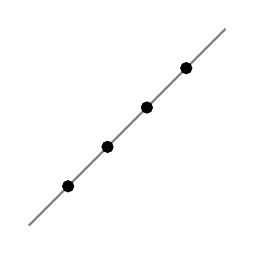
\begin{tikzpicture}
    % \draw[gray, thick] (-1,2) -- (2,-4);
    \draw[gray, thick] (-0.5,-0.5) -- (2,2);
    \filldraw[black] (0,0) circle (2pt);
    \filldraw[black] (1,1) circle (2pt);
    \filldraw[black] (0.5,0.5) circle (2pt);
    \filldraw[black] (1.5,1.5) circle (2pt);
\end{tikzpicture}
\caption{Example of setup where $|X|$ term dominates and $I \sim |X|$}
\label{fig:example1st}
\end{figure}
\end{example}

\begin{example}[Example 2 for ST Theorem]
    The ST theorem is sharp with the $|L|$ bound when the number of lines is large and each line lies on a single point.


\begin{figure}[h]
    \centering
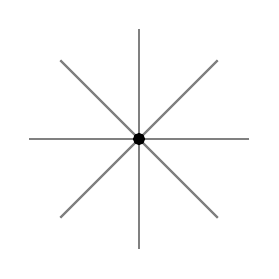
\begin{tikzpicture}
    % \draw[gray, thick] (-1,2) -- (2,-4);
    \draw[gray, thick] (-1,-1) -- (1,1);
    \draw[gray, thick] (1.4,0) -- (-1.4,0);
    \draw[gray, thick] (0,1.4) -- (0,-1.4);
    \draw[gray, thick] (1,-1) -- (-1,1);
    \filldraw[black] (0,0) circle (2pt);
\end{tikzpicture}
\caption{Example of setup where $|L|$ term dominates and $I \sim |L|$. }
\label{fig:example2st}
\end{figure}
\end{example}

\begin{example}[Example 3 for ST Theorem]
    


We let $X$ be an $N\times N$ grid, and define $Q_M := \{\frac{a}{b} : a,b \in  [M]\}$. Define $L$ to be the set of lines with slopes in $Q_M$ that pass through points in $X$. Then $|Q_M| \sim M^2$ (the double counting when $\gcd(a,b) > 1$ only affects the magnitude of $|Q_M|$ up to a constant factor). Every point in $X$ has a line passing through it for each slope in $Q_M$. Then 


\begin{equation}
I(X,L) =|X| |Q_M| \sim N^2 M^2
\end{equation}

We now define projection operators for each $s\in Q_M$ as 

\begin{equation}
\pi_s(x_1, x_2) = x_2 = -sx_1
\end{equation} 

The fibers of $\pi_s$ are lines of slope $s$, and the number of lines in $L$ with direction $s$ is $|\pi_s(X)|$. We now prove the following lemma: 

\begin{lemma}
    For all $s\in Q_M$, $|\pi_s(X)| \lesssim MN$
\end{lemma}

\begin{proof}
Take $x_1, x_2 \in [N]$ and $s = \frac{a}{b} $. Then 

\begin{equation}
\pi_s(x_1, x_2) = x_2 - \frac{a}{b} x_2 = \frac{bx_2 - ax_1}{b} 
\end{equation}

Since $a,b \leq M$ and $x_1, x_2 \leq N$, $|bx_2 - ax_1| \lesssim MN$. Since $bx_2 - ax_1$ must be an integer, there are at most $MN$ distinct values in $\pi_s(X)$. 
\end{proof}

Then since $L$ has at most $NM$ lines for every element of $Q_M$. $|L \lesssim |Q_M|NM \sim M^3 N$. Then 

\begin{equation}
I(X,L) \sim N^2 M^2 \gtrsim (M^3 N \cdot N^2)^{2/3} \gtrsim |X|^{2/3} |L|^{2/3}
\end{equation}

Therefore the grid is a sharp example of the Szemerédi–Trotter theorem where the $|X|^{2/3}|L|^{2/3}$ term dominates. Note that the Szemerédi–Trotter theorem implies the ST projection theorem, which is a special case when $L$ is the set of lines with directions in $D$ passing through points in $X$. 


\end{example}

\subsection{Question: Are there other sharp examples for the Szemerédi–Trotter theorem?}

Another example is grids over number fields. Let $R$ be a number field, (for example $\mathbb{Z}[\sqrt{2 }]$). Then define 

\[R_N = \{a_1 + a_2 \sqrt{2}: a_1, a_2 \in \mathbb{Z}, |a_1|, |a_2| \leq N\}\]

\[QR_M = \{\frac{a}{b}: a,b \in R_M\}\]

Then define $X:= R_N \times R_N$ and $L$ as the set of lines with slopes in $QR_M$ that pass through a point in $X$. This is similar to the grid example. 

\subsection{Proof of the Szemeredi-Trotter theorem}

We begin the proof of the Szemeredi-Trotter theorem with a lemma. 

\begin{lemma}
\begin{displaymath}
I(X,L) \leq |X| |L|^{1/2} + |L|
\end{displaymath}
\label{weak_bound_ST_lemma}
\end{lemma}
\begin{proof}
We start with expanding $I(X,L)$ and applying Cauchy Schwartz to get 

\[I(X,L) = \sum_{\ell \in l} |\ell \cap X| \leq \left(|L|\sum_{\ell \in L} |\ell \cap X|^2 \right)^{1/2}\]


This is advantageous because $|\ell \cap X|^2 \lesssim \binom{|\ell \cap X|}{ 2} + 1$. Then 

\[\sum_{\ell \in L} |\ell \cap X|^2  \lesssim |L| + \sum_{\ell \in L} \binom{|\ell \cap X|}{2}  \] 

Since for every pair of points $x_1, x_2 \in X$, there is at most one line $\ell$ that contains $x_1$ and $x_2$, every pair of points in $X$ can be counted at most once. Then 

\[ \sum_{\ell \in L} \binom{|\ell \cap X|}{2} \leq \binom{|X|}{2} \lesssim |X|^2\]

This gives the final conclusion 

\[I(X,L) \lesssim \left(|L| (|X|^2 + |L|)\right)^{1/2} \leq |X||L|^{1/2} + |L|\]

\end{proof}

Note that this proof uses only the very general fact that any two points define a line. Therefore it holds over spaces such as finite fields. However, the Szemerédi–Trotter theorem does not hold over finite fields. To see this take $X = \mathbb{F}_q^2$ (as the whole space) and $L$ as all lines in $\mathbb{F}_q^2$. Then for every $\ell$, $|\ell \cap X| = q$, so $I(X,L) = q^3$. However, $|X|^{2/3} |L|^{2/3} = q^{8/3} \leq I(X,L)$. Therefore, the Szemerédi–Trotter theorem requires properties of the topology of $\mathbb{R}^2$ to work. In particular, it uses a cell decomposition lemma, which allows cutting the plane into pieces. 

\begin{lemma}[Cell decomposition lemma]
Let $X$ be a set of points in $\mathbb{R}^2$ and pick an integer $s\geq 1$. Then the plane can be disjointly partitioned into a set of open sets $O_i$ and a closed set $W$ such that 

\[\mathbb{R}^2 = W \cup \bigcup_i O_i\] 

and additionally, 

\[|\ell \cap W| \leq s\] 

and for every $i$, 

\[|X| \cap O_i| \lesssim \frac{|X|}{s^2} \]
\end{lemma}

This lemma essentially states that the plane can be split into cells that each contain only a small subset of $X$, and that the walls don't intersect any line too many times. As an example of this theorem, let $X$ be a "roughly" square grid. That is $\subset [N]^2$ and fir every ball $B_1(c)$ of radius 1 (where $c$ is an arbitrary point in the plane), $|X\cap B_1(c)| \lesssim 1$. The below example shows the grid for $s = 2$. 

\begin{figure}[h]
    \centering
    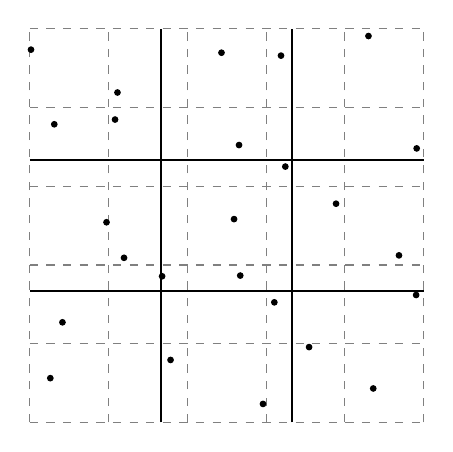
\begin{tikzpicture}
        % \draw[gray, thick] (-1,2) -- (2,-4);
        \foreach \i in {0,1,2,3,4,5} {
        \draw[gray, dashed] (0,\i) -- (5,\i);
        \draw[gray, dashed] (\i,0) -- (\i,5);
        }
        \foreach \i in {5/3, 10/3} {
            \draw[black, thick] (0,\i) -- (5,\i);
            \draw[black, thick] (\i,0) -- (\i,5);
        }
        \filldraw[black] (0.25955310498674833, 0.5630661519871801) circle (1pt);
        \filldraw[black] (0.4137916302144814, 1.2720619913477607) circle (1pt);
        \filldraw[black] (0.9732231939725711, 2.5427334886772703) circle (1pt);
        \filldraw[black] (0.3098666106054, 3.7871072206930636) circle (1pt);
        \filldraw[black] (0.01419593145904452, 4.734899395195148) circle (1pt);
        \filldraw[black] (1.786606807737972, 0.79422295279698) circle (1pt);
        \filldraw[black] (1.67931813829752, 1.8571052177749485) circle (1pt);
        \filldraw[black] (1.1956960247777007, 2.0912689126469677) circle (1pt);
        \filldraw[black] (1.0815919550119522, 3.847137097298062) circle (1pt);
        \filldraw[black] (1.112216822269262, 4.190692648040198) circle (1pt);
        \filldraw[black] (2.9605994936072006, 0.23571202532548774) circle (1pt);
        \filldraw[black] (2.6718713017136357, 1.865754141181469) circle (1pt);
        \filldraw[black] (2.593013450706421, 2.582698705322111) circle (1pt);
        \filldraw[black] (2.6562500412019583, 3.523426303538553) circle (1pt);
        \filldraw[black] (2.4334135790739353, 4.696110600325106) circle (1pt);
        \filldraw[black] (3.546029544303023, 0.9573850322061107) circle (1pt);
        \filldraw[black] (3.1047794604515966, 1.5257811772946877) circle (1pt);
        \filldraw[black] (3.888160864908276, 2.7785089574468333) circle (1pt);
        \filldraw[black] (3.2442635963634507, 3.249918857886983) circle (1pt);
        \filldraw[black] (3.1892303954436376, 4.65910033789462) circle (1pt);
        \filldraw[black] (4.360650110813351, 0.43213244516574956) circle (1pt);
        \filldraw[black] (4.905246089511404, 1.6192226713487996) circle (1pt);
        \filldraw[black] (4.687574700923156, 2.122352916188249) circle (1pt);
        \filldraw[black] (4.912275419613345, 3.480674850602295) circle (1pt);
        \filldraw[black] (4.300124921435576, 4.907912984137379) circle (1pt);
    \end{tikzpicture}
    \caption{The points show the points in $X$. The dashed lines indicate the "rough grid" shape of $X$. The solid lines show $W$, which is the set dividing $X$}
    \label{fig:gridcells}
\end{figure}

Each line can only intersect $2s$ lines in $W$, so $|\ell \cap W| \leq 2s$. Since $X$ is roughly grid shaped, and each cell is a square of side length $N/s$, $|X\cap O_i| \lesssim |X|/s^2$, which satisfies the requirements. 

We now proceed to the proof of the Szemerédi–Trotter theorem. It hinges on the fact that lemma \ref{weak_bound_ST_lemma} is sharp when the number of lines is either small (bounded by a constant) or much larger than the number of points $(|L| > |X|^2)$. We can use this by using the cell decomposition lemma to pick cells where one of these conditions holds. 

\begin{proof}
Given $X$ and $L$, and arbitrary $s$. Then using the cell decomposition lemma, define $X_i = X \cap O_i$. Then $|X_i| \leq |X|/s^2$ and 

\[\sum_i |X_i| \leq |X|\] 

Define 

\[L_i = \{\ell \in L: \ell \cap O_i \neq \emptyset\}\]


From the cell decomposition lemma

\[\sum_i |L_i| \leq s |L|\]

Then as every intersection of a point and a line is either on a cell boundary or within a cell. Then 

\[I(X,L) \leq \sum_i I(X_i, L_i) + I(X\cap W, L)\] 

Applying lemma \ref{weak_bound_ST_lemma} to the first term, and the $|\ell \cap W| \lesssim s$ bound to the second term, 

\begin{align*}
    I(X,L) \lesssim & \sum_i (|X_i| |L_i|^{1/2} + |L_i|) + s|L|\\
    \lesssim & \left(\sum_i |X_i|^2 \sum_i |L_i|\right)^{1/2}+ 2s|L|\\
    \lesssim & \left(\sum_i \frac{|X|}{s^2} |X_i| \right)^{1/2}(s|L|)^{1/2} + 2s|L|\\
    \lesssim & s^{-1/2} |X| |L|^{1/2} + s|L|\\
\end{align*}

We then choose $s$ to minimize this quantity. This is effectively choosing $s$ so that both terms are equal. Then 

\begin{align*}
    s^{-1/2} |X| |L|^{1/2} = & s|L|\\
    |X||L|^{-1/2} = & s^{3/2}\\
    s = & |X|^{2/3} |L|^{-1/3}
\end{align*}

 Plugging $s$ back into the inequality gives 


\[I(X,L) \lesssim |X|^{2/3}|L|^{2/3}\]  

which gives the desired bound.
\end{proof}

 Note that in the above argument $s$ must be an integer, so this can only be done when $|X|^2 > |L|$. When $|X|^2 < |L|$ then setting $s = 1$ gives the the bound $I(X,L) \lesssim |L|$. Additionally, $s^2$ can be at most $|X|$. Then when $|X| <  |X|^{4/3} |L|^{-2/3}$, $|X| > |L|^2$, so setting $s =|X|^{1/2}$ gives the bound $I(X,L) \lesssim |X|$


We now prove the cell decomposition lemma. However, several prelimary theorems must be shown first. 

\begin{theorem}[Borsuk Ulam Theorem]
Let $f: S^n \to \mathbb{R}^n$ be a continuous function that is antipodal, ie for every $\theta \in S^n$, $f(\theta) = -f(- \theta)$. Then 0 is in the image of $f$. 
\end{theorem}

\begin{Corollary}[Ham Sandwich Theorem]
    Let $O_1, O_2, ..., O_n \subset \mathbb{R}^n$ be bounded open subsets. Then there exists a hyperplane $H$ that bisects every $O_i$. 
\end{Corollary}

\begin{proof}
An upper half (hyper)plane can be described as the set $\{x: a \cdot x > b\}$, for some vector $a$ and $b$ a real number. As scaling $a$ and $b$ by a positive real number preserves this hyperplane, the tuple $(a,b)$, can be identified with an element of $S^n$. Then for an element $\theta \in S_n$ corresponding to $(a,b)$, we let $c_\theta$ be the affine operator defined by $c_\theta(x) = a\cdot x + b$. We then define the vector valued function $f$ by

\[f_i(\theta) = \text{Vol}(O_i \cap \{x: c_\theta(x) > 0\}) - \text{Vol}(O_i \cap \{x: c_\theta(x) < 0\})\] 

$f$ is antipodal, so it has a zero. This zero corresponds to each set being bisected, which proves the theorem
\end{proof} 

The Ham Sandwich theorem works when there are up to $n$ subsets of $\mathbb{R}^n$. This is roughly because $n$ degrees of freedom are needed to bisect the $n$ sets. We can then use polynomials to increase the number of degrees of freedom, and so the number of sets that can be bisected. 

\begin{theorem}[Polynomial Ham Sandwich Theorem]
    We use the same setup as the ham sandwich theorem, except that there can be up to $N$ sets $O_i$. Then there exists a polynomial zero set that bisects every $O_i$
\end{theorem} 

\begin{proof}

    First define the space 

    \[\text{Poly}_D(\mathbb{R}^n) = \{p \in \mathbb{R}[x_1, ..., x_n]: \deg  p \leq D\}\]

    $\text{Poly}_D(\mathbb{R}^n)$ is then a vector space of degree $D^n$. We claim that if $N < D^n$, then there is a nonzero element of $\text{Poly}_D(\mathbb{R}^n)$ that satisfies the claim. We define the vector valued function $f$ by 

    \[f_i(p) = \text{Vol}(O_i \cap \{x: p(x) > 0\}) - \text{Vol}(O_i \cap \{x: p(x) < 0\})\] 

    Since scaling each nonzero $p$ by a positive real does not change $f$, $f$ is a function from $S^{D^{N}-1}$ to $\mathbb{R}^n$. Additionally, $f$ is antipodal. Then by the Borsuk Ulam theorem the conclusion follows. 
\end{proof}

The Ham Sandwich theorems allow open subsets of Euclidean space to be subdivided, but the cell decomposition lemma requires dividing sets of points. This is a technical detail that follows from the Polynomial Ham Sandwich Theorem. 

\begin{lemma}[Ham Sandwich theorem for finite sets]
Let $s_1,s_2,... ,s_N$ be a set of finite sets in $\mathbb{R}^n$. Then there exists a polynomial level set such that for every $s_i$, 

\[|s_i \cap \{x: p(x) > 0\}| \leq \frac{|s_i|}{2} \]
\[|s_i \cap \{x: p(x) < 0\}| \leq \frac{|s_i|}{2} \]
\end{lemma}

As individual points cannot be bisected, this lemma instead guarantees that excess points will lie on the level set. 

\begin{proof}
Take some $\epsilon > 0$ and for each $i$ define $N_\epsilon(s_i)$ to be the set of balls of radius $\epsilon$ centered at the points on $s_i$. Then by the Polynomial Ham Sandwich theorem the $N_\epsilon(s_i)$ can all bisected by the zero set of a polynomial of degree $D^n > n$. Then taking $\epsilon$ to 0 we get a sequence of polynomials $p_\epsilon$ that each bisect the $N_\epsilon(s_i)$. Since the sphere $S^n$ is compact, there must a convergent subsequence to some polynomial $p$. To show that this polynomial $p$ satisfies the conclusion, for contradiction assume that there exists $i$ such that

\[|s_i \cap \{x: p(x) > 0\}| > \frac{1}{2} |s_i|\] 

Since every point in $s_i \cap \{x: p(x) > 0\}$ is some nonzero distance from the set $\{x: p(x) = 0\}$, there is some $\epsilon > 0$ such that modifying $p$ by $\epsilon$ and enlarging $s_i$ by $\epsilon$ gives 

\[|N_\epsilon(s_i) \cap \{x: p_\epsilon(x) > 0\}| > \frac{1}{2} |N_\epsilon(s_i)| = \] 

a contradiction. Note that this step requires the boundedness of $s_i$ to take a perturbation of $p$ continuous. 
\end{proof}

We will now prove the cell decomposition lemma. 

\begin{proof}
    We begin with step $k=1$. Then define $p_1$ to be the degree 1 polynomial that splits $X$ into two parts. Then $X_{1,1} := \{x \in X:  p_1(x) > 0\}$ and $X_{1,2} := \{x \in X:  p_1(x) < 0\}$

    Then at stek $k+1$, define $p_k$ to be the polynomial of degree $D_k$ with $D^2 \sim 2^{k}$ such that $p_k$ bisects all $X_{k,1},..., X_{k, 2^k}$. Then $D_k \sim 2^{k/2}$. 

    Then pick $k_{final} $ such that $2^{k_{final}} \sim s^2$. Then let $O_i$ be the sets defined by $\{x: \pm p_1(x) > 0\}  \cap ... \cap \{x: \pm p_{k_{final}}(x) > 0\}$ for all choices of $\pm$. Define $W = \{x: p_1(x) = 0\} \cup ... \cup \{x: p_{k_{final}}(x) = 0\}$
    
    $X$ has been bisected $k_{final}$ times, so then 

    \[|X_{k_{final}, i}| \lesssim |X|/s^2\] 

    A line can intersect a polynomial of degree $D$ at most $D$ times, so then 

    \[|\ell \cap W| \leq 1 + 2 + 4 + ... + 2^{k_{final}/2} \sim s \]

    Then each line can intersect $W$ at most $\sim s$ times. 
\end{proof}

\newpage


\section{Reflections on the Szemeredi-Trotter theorem}

Thur March 6

There is an important analogy between the Szemeredi-Trotter theorem and the exceptional set problem in projection theory.   The Szemeredi-Trotter theorem can be viewed as the sharp projection theorem for finite sets of points in $\RR^2$.   The exceptional set problem concerns the projection theory of a finite set of balls in $\RR^2$ subject to a natural spacing condition.   The sharp answers to both problems are essentially the same -- based on integer grids.   This analogy was noticed by Tom Wolff in the late 1990s.   He adapted proof methods from combinatorial geometry to problems in geometric measure theory and harmonic analysis,  with striking results.   He tried hard to adapt the proof of Szemeredi-Trotter to the exceptional set problem and the Furstenberg set conjecture,  but he was not able to prove sharp results.   

The proof of Szemeredi-Trotter using topological methods is elegant and important,  but there are several important questions that it does not address.  In this class we will discuss them.   



First let's recall the statement of Szemer\'edi-Trotter theorem. Let $X$ be a set of points, $L$ be a set of lines (both in $\mathbb{R}^2$), we use $I(X,L)$ to denote the set of incidences between them:
\begin{equation*}
    I(X,L) = \{(p,l) \in X \times L: p \in L\}.
\end{equation*}
Szemer\'edi-Trotter claims that 
\begin{equation*}
    |I(X,L)| \lesssim |X| + |L| + |X|^{2/3} |L|^{2/3}.
\end{equation*}

All the current proofs of this theorem, like the cell decomposition method we discussed in the previous lectures, used the topology of Euclidean plane. This is not surprising, as the conclusion of this theorem is indeed related to the structure of the base field. If we replace $\mathbb{R}^2$ by $\mathbb{F}_p^2$, Szemer\'edi-Trotter bound will fail as one can see by taking $L$ to be all the lines in $\mathbb{F}_p^2$. 

On the other hand, the current methods provide little information on some closely related problems, such as:

1. Projection theory over finite fields. 

2. Structure of sharp examples for Szemer\'edi-Trotter. 

3. Projection theory of unit balls, instead of points, in $\mathbb{R}^2$ with spacing conditions (lots of attempts by Wolff). 

\subsection*{Structure of Sharp Examples}

Let's stare at the Szemer\'edi-Trotter bound:
\begin{equation*}
    |I(X,L)| \lesssim |X| + |L| + |X|^{2/3} |L|^{2/3}.
\end{equation*}
There are three terms on the RHS. The first two terms are given by double counting which generalizes to other fields. They dominate when there are too many points or lines, in which case the structure of the sharp examples example is not very rigid, giving us many degrees of freedom.  To be more specific, when the first dominates we have $|X| \gg |L|^2$, which means that the number of points has already exceeded the total number of intersections among the lines. In this case, the upper bound is tight if each point has a line passing through it. The typical sharp example looks like some chains of beads. Similarly, when the second term dominates the sharp examples look like a bunch of stars, where each line doesn't have much chance to pass through too many points.

The case where the third term dominates is the most interesting one. The known sharp examples are integer grids and their variation $R$-grids, where $R$ is the integer rings of number fields. We expect that the sharp examples in this case are highly structured. To see what information about the sharp examples the proof of Szemer\'edi-Trotter theorem tells us, let's briefly review the cell decomposition proof: Divide $\mathbb{R}^2$ into $s^2$ cells. In each cell there are $|X|/s^2$ points and (in average) $|L|/s$ lines. By choosing $s$ to be large enough we will have $|L|/s \gtrsim (|X|/s^2)^2$ and then apply the double counting bound. The proof doesn't tell us much information on the structure of the sharp example unless we can figure out the way our cells interact. Unfortunately the proof of cell decomposition is not very constructive and based on existence theorems from topology.

\begin{remark}
    In the projective plane $\mathbb{P} \mathbb{R}^2$ there is something called point-line duality. It preserves the incidence relationship between points and lines. In fact, the statement that a point with coordinates $[a_0, a_1 , a_2]$ lies on a line with coefficients $[b_0, b_1, b_2]$ simply means $a_0 b_0 + a_1 b_1 +  a_2 b_2 = 0$, where the roles of $a_i$ and $b_i$ are interchangeable. The chain example and the star examples are mapped to each other via the point-line duality, while  the grid example will be mapped to something different. 
\end{remark}

There are also some interesting variations of this problem. For example, one may ask about the structure of $X$ which maximizes the projections for some particular $D$. Define $S_D(N) = \min_{|X|=N} S(X,D)$. For an arbitrary $D$, what can we tell about the structure of $X$ achieving this maximum? All the known examples are for direction sets with special structures.  

Denote the directions in $\mathbb{R}^2$ by elements of $\mathbb{R} \cup \{\infty\}$ with corresponding projections $\pi_t(x) = x_1+tx_2$ for $t \in \mathbb{R}$, $\pi_\infty(x) = x_2$. Since we can use a projective transformation to map any three directions to any three specified directions without changing the incidence structure, let's begin with $|D|=4$. Without of loss of generality we may assume $D = \{0,1,t,\infty\}$. When $t$ is rational with small denominator the grid example still works. Things become more interesting when $t$ is transcendental. For example, we may take $P_{k,s} = \{a_0 + a_1 t + \cdots + a_{k-1} t^{k-1}: a_i \in \mathbb{Z}, 0 \le a_i \le s-1\}$ be a set of polynomials in $t$ and let $X = P_{k,s} \times P_{k,s}$. Then $|X| = s^{2k}$. We have $\pi_0(X) = \pi_\infty(X) = P_{k,s}$, $\pi_1(X) \subset P_{k,2s}$, $\pi_t(X) \subset P_{k+1,2s}$. Since $t$ is transcendental, $S(X,D) \sim |\pi_t(X)| \sim  2^k |X|^{1/2k} |X|^{1/2}$. Choose $k = (\log_2(|X|)/2^{1/2}$ to maximize the RHS, we obtain that is this case $S_D(X) \sim e^{c(\log|X|)^{1/2}} |X|^{1/2}$. It would also be interesting to analyze $S(X,D)$ for other $D$'s, like $D=\{0,1,\infty,t_1,\ldots,t_k\}$ where $t_j$'s are algebraic independent over $\mathbb{Q}$.

\subsection*{Projection Theory over Finite Fields}

We have seen that projection theory over finite fields may be different from that over the reals. Let $X$ be a set of points, $D$ be a set of directions. Let $S = \max_{\theta \in D} \pi_\theta(X)$. Our conjecture is that for $|S| \le p/2$, 
\begin{equation*}
    |S| \gtrsim |D|^{1/2} |X|^{1/2}.
\end{equation*}
It would be attempting to investigate the structure of sharp examples for this bound, and one may conjecture they are essentially grids. 

\begin{remark}
    Let's give an example showing that the original version of Szemer\'edi-Trotter bound fails over complex field. Again, let $X$ be a set of unit balls in $B_R^{\mathbb{C}^2} \subset \mathbb{C}^2$, $D \subset B_1^\mathbb{C} \subset  \mathbb{C}$ be an $R^{-1}$-separated set of directions. For $t \in D$, let $\pi_t: \mathbb{C}^2 \to \mathbb{C}$ be the map $(z_1, z_2) \mapsto z_1 + t z_2$. For our example, choose $X$ to be a maximal set of $R^{-1}$-separated unit balls with centers in $\mathbb{R}^2$, and $D$ to be a maximal $R^{-1}$-separated subset of $\mathbb{R} \cap B_R^\mathbb{C}$. Then $|X| \sim R^2$, $|D| \sim R$ satisfy the Hausdorff spacing condition, while $S(X,D) \sim R \ll |X|^{1/2} |D|^{1/2}$.
\end{remark}

\subsection*{Projection Theory of Unit Balls}

Let $X$ be a set of unit balls in $B_R$, $D$ be a set of $1/R$-separated directions. Define $N_X(r) = \max_{c \in B_R} |X \cap B(c,r)|$, $N_D(\rho) = \max_{\gamma \subset \mathbb{S}^1, |\gamma| = \rho} |D \cap \gamma|$. We will assume that $X$ has Hausdorff spacing, which means there exists $0 \le \alpha \le 1$ such that $|X| \sim R^\alpha$, $N_X(r) \lesssim r^\alpha$. Similarly we will also assume that $|D| \sim R^\beta$, $N_D(r/R) \lesssim r^\beta$. The following conjecture by Furstenberg was recently proved by Orponen, Shmerkin, Ren and Wang:

\begin{theorem}
    Under the above assumption, we have 
    \begin{equation*}
        |D| \stackrel{<}{\approx} |S|^2/|X|
    \end{equation*}
    if $|D| \lesssim R^{-\epsilon}\min(R,|X|)$.
\end{theorem}

We will discuss briefly why cell decomposition doesn't work in this case. Suppose that we have divided $B_R$ into $s^2$ cells. There is no guarantee on the shape of each cell $O_i$, but in one important scenario, most cells   are roughly balls of some radius $r$ so that it is possible for us to apply induction hypothesis. (At first one might think $r = R/s$, but this may not be the case.  It may be that most of the balls of radius $r$ cover only a fractal subset of $B_R$ which contains our set $X$.)  
The problem is, the $R^{-1}$-separated directions may look indistinguishable at smaller scales. In each cell we have to choose an $r$-separated subset $D_i \subset D$. By the Hausdorff assumption, in a typical cell we will have $|X_i| \sim r^\alpha$, $|D_i| \sim r^\beta$. So we can not force $|X_i|^2$ to be smaller than $|L_i|$ by simply passing to smaller balls.

\newpage


\section{Sum-product theory}

Tues March 18

The best bounds in projection theory are different in different fields.  The best bounds for projections of balls in $\CC^2$ are different than in $\RR^2$.   The best bounds for projections in $\FF_{p^2}^2$ are different than for $\FF_p^2$.   Most of the recent work in projection theory is concerned with understanding these differences,  and they are important for many applications.

The key example is simplest in the finite field setting.  It goes as follows.  

\begin{example}\label{eg:1.1}
    Let $p$ be a prime, $q=p^2$, $X=\F_p^2\subset\F_q^2$, $D=\F_p\subset\F_q$. For $\theta\in\F_q$, let $\pi_\theta:\F_q^2\to\F_q$ be defined by $\pi_\theta(x_1,x_2)=x_1+\theta x_2$. Then set $S=\max_{\theta\in D}|\pi_\theta(X)|$. We have $\pi_\theta(X)=\F_p$ for all $\theta\in D$, so $S=p$. Then we have $|X|=p^2=q,S=|D|=p=q^{1/2}$. 
\end{example}

So the sizes of the projections of $X$ can be small even when $X$ is large. However, the same cannot happen over $\F_p$:

\begin{theorem}[Bourgain-Katz-Tao]\label{thm:bkt}
    Let $X\subset\F_p^2$ with $|X|=p^s$ for $0\leq s<2$. Let $D\subset\F_p$ with $|D|=p^t$ for $0<t\leq 1$. Then $S=\max_{\theta\in D}|\pi_\theta(X)|\geq p^{s/2+\eps(s,t)}$ where $\eps(s,t)>0$.
\end{theorem}

There is an example in $\CC^2$ which is analogous to Example \ref{eg:1.1}.   In this example $X = \RR^2 \subset \CC^2$.   And there is a theorem called the Bourgain projection theorem which says that no set in $\RR^2$ can behave similarly to this example.  We will dicuss the Bourgain projection theorem in detail in a few lectures.   We begin with the finite field setting which is somewhat cleaner.   The setting of balls in $\RR^2$ is analogous with some additional issues.


Note that the key difference between $\F_p$ and $\F_q$ that allows an example like Example \ref{eg:1.1} to exist while no such example exists over $\F_p$ is the existence of a subfield $\F_q$. A way to quantify the properties of a subfield is a set $X$ with small sum and product sets. As such, we should study the sizes of such sets.   This study is called sum-product theory.   

Sum-product theory uses tools from additive combinatorics.   The set of tools that go into the proof of Theorem \ref{thm:bkt} is very different from the tools that we have studied in projection theory so far.   In this lecture,  we introduce sum-product theory and some of the key tools from additive combinatorics.   This is the first of four lectures on this area.   Over the four lectures we will flesh out the different tools from the area and use them to prove the BKT projection theorem.



\subsection{Sum-product theory}

\begin{notation}
    For $A\subset\F_p$, let
    $$A+A=\{a_1+a_2:a_i\in A\},\quad A\cdot A=\{a_1a_2:a_i\in A\}.$$
    Also, let $A^{\oplus n}=\underbrace{A+A+\dots+A}_n$.
\end{notation}


If $A$ is an arithmetic progression,  then its sumset is only a little bigger than $A$.   If $A$ is a geometric progression, then its product set is only a little bigger than $A$.   Erdos and Szemeredi conjectured that for any set of numbers $A$,  either the sumset or the product set is much bigger than $A$.   This principle has turned out to be crucial for modern developments in projection theory.   We introduce this subject,  including a whole different set of tools from combinatorial number theory building on work of Plunnecke, Ruzsa and Edgar-Miller.

\begin{lemma}\label{lem:1}
    If $A\subset\F_p$, then either
    \begin{enumerate}
        \item $\frac{A-A}{A-A}=\F_p$, or
        \item $\left|\frac{(A\cdot A)^{\oplus 3}-(A\cdot A)^{\oplus 3}}{A-A}\right|\geq|A|^2$.\label{2}
    \end{enumerate}
\end{lemma}

Remark.  Some version of this trick goes back to the work of Edgar-Miller,  and it was adapted by Bourgain-Katz-Tao and Garaev.

\begin{proof}
    First, note that if $c\not\in\frac{A-A}{A-A}$, then $|A+cA|=|A|^2$. Indeed, if this was not the case then there would be some $a_1,a_2,a_1',a_2'\in A$ with $a_1+ca_2=a_1'+ca_2'$. But this implies $c=\frac{a_1'-a_1}{a_2-a_2'}\in\frac{A-A}{A-A}$.

    Next, note that if $\frac{A-A}{A-A}\neq\F_p$ then there is some $b\in\frac{A-A}{A-A}$ with $b+1\not\in\frac{A-A}{A-A}$. Indeed, we can set $b+1$ to be the smallest element of $\F_p\setminus\frac{A-A}{A-A}$, which would imply $b\in\frac{A-A}{A-A}$.

    Now, if $\frac{A-A}{A-A}\neq\F_p$, then we have
    $$\left|A+\left(\frac{A-A}{A-A}+1\right)A\right|\geq|A|^2,$$
    which implies \ref{2} after putting the LHS over a common denominator.
\end{proof}

\subsection{Freiman-Ruzsa theorem}

One question to ask in sum-product theory is when the set $A+A$ is small.

\begin{example}
    \begin{enumerate}
        \item If $A=[L]$, then $|A+A|\leq 2|A|$.
        \item More generally, if $A$ is an arithmetic progression $A=\{a+nd\}_{n\in[L]}$, then $|A+A|\leq 2|A|$.
        \item Even more generally, we can consider $A=\{a+n_1d_1+\dots+n_rd_r\}_{n_i\in[L_i]}$. Then $A+A\subset\{2a+n_1d_1+\dots+n_rd_r\}_{2\leq n_i\leq 2L_i}$, so $|A+A|\leq 2^r|A|$. In this case we call $A$ a \textbf{generalized arithmetic progression (GAP)} of dimension $r$ and volume $L_1\cdots L_r$.
    \end{enumerate}
\end{example}

\begin{theorem}[Freiman-Ruzsa]
    If $A\subset\Z$ and $|A+A|\leq K|A|$, then $A$ is contained in a GAP of dimension $r(K)$ and $\vol\leq V(K)\cdot|A|$.
\end{theorem}

This is a deep theorem that we will not prove, and the quantitative bounds on $r(K)$ and $V(K)$ are weak. In the original paper, the bounds were of the form $r(K)=\exp(K^c),V(K)=\exp(\exp(K^c))$, so the theorem is only meaningful if $K$ is small.

\begin{conj}
    There is a meaningful bound if $K=|A|^\delta$ for some $\delta>0$.
\end{conj}

\subsection{Ruzsa triangle inequality}

\begin{theorem}[Ruzsa]
    Let $Z$ be an abelian group and $A,B,C\subset Z$. Then $|A||B-C|\leq|A-B||A-C|$.
\end{theorem}

\begin{corollary}
    If $|A+A|\leq K|A|$, then $|A-A|\leq K^2|A|$.
\end{corollary}
\begin{proof}
    Use Ruzsa's triangle inequality with $A=A,B,C=-A$. Then we have
    $$|B-C|=|(-A)-(-A)|=|A-A|,\quad|A-B|=|A-C|=|A-(-A)|=|A+A|.$$
    So Ruzsa's triangle inequality tells us that $|A||A-A|\leq|A+A|^2$, which implies the corollary.
\end{proof}

\begin{proof}[Proof of Ruzsa triangle inequality]
    We will construct an injective map $\phi:A\times (B-C)\to(A-B)\times(A-C)$. For all $d\in B-C$, fix some $b(d)\in B,c(d)\in C$ with $d=b(d)-c(d)$. Then set $\phi(a,d)=(a-b(d),a-c(d))$. We need to show that $\phi$ is injective. Suppose $\phi(a,d)=(x,y)$. Then we will recover $a,d$ from $x,y$ and the choices of $b(d),c(d)$. Note that we have $y-x=b(d)-c(d)=d$, so we can recover $d$. Then from $d$ we know $b(d)$, so we can recover $a=x+b(d)$.
\end{proof}

\subsection{Plunnecke inequality}

\begin{theorem}[Plunnecke]
    Let $Z$ be an abelian group and $A,B\subset Z$ with $|A+B|\leq K|A|$. Then $|B^{\oplus m}-B^{\oplus n}|\leq K^{m+n}|A|$.
\end{theorem}

\begin{corollary}
    If $|A+A|\leq K|A|$ then $|A-A|\leq K^2|A|$, $|A+A+A|\leq K^3|A|$.
\end{corollary}

\begin{corollary}
    If $|A-A|\leq K|A|$ then $|A+A|\leq K^2|A|$.
\end{corollary}
\begin{proof}
    Use Plunnecke's inequality with $B=-A$.
\end{proof}

\begin{lemma}\label{lem:2}
    If $A\subset\F_p,|A|=p^s$ for $0\leq s<1$, then $|A^3-A^3|\geq p^{s+\eps(s)}$ for some $\eps(s)>0$.
\end{lemma}
\begin{proof}
    Let $B=(A^2)^{\oplus 3}-(A^2)^{\oplus 3},C=A-A$. Then by Lemma \ref{lem:1} we have $\left|\frac{B}{C}\right|\geq p^{s+\gamma(s)}$ for some $\gamma>0$. Now, assume for contradiction that $|A^3-A^3|\leq K|A|$ where $K\lessapprox 1$. Then we have $|A^3|\leq K|A|$, and since $|A|\leq|A^3|$, we have $|A^3-A^3|\leq K|A^3|$. Then Plunnecke's inequality implies
    $$|(A^3)^{\oplus m}-(A^3)^{\oplus n}|\leq K^{m+n}|A^3|\leq K^{m+n+1}|A|.$$
    In particular, this implies $|B\cdot C|,|A\cdot B|,|A\cdot C|\leq K^{O(1)}|A|$. Then the Ruzsa triangle inequality (on $\F_p$ as a multiplicative set) implies
    $$|A|\left|\frac{B}{C}\right|\leq|A\cdot B||A\cdot C|\leq K^{O(1)}|A|^2,$$
    so we have $p^{s+\gamma}\leq\left|\frac{B}{C}\right|\leq K^{O(1)}|A|=K^{O(1)}p^s$, which contradicts $K\lessapprox 1$.
\end{proof}

In fact, there is actually a stronger statement:

\begin{theorem}[Bourgain-Katz-Tao]
    If $A\subset\F_p$ with $|A|=p^s$, then $\max(|A\cdot A|,|A+A|)\geq p^{s+\eps(s)}$.
\end{theorem}

\begin{notation}
    We define $\poly_K(A)=(A^K)^{\oplus K}-(A^K)^{\oplus K}$.
\end{notation}

\begin{corollary}
    If $0<s<t<1$, then there exists a $K=K(s,t)$ such that for all $A\subset\F_p$ with $|A|=p^s$, we have $|\poly_K(A)|\geq p^t$.
\end{corollary}
\begin{proof}
    Apply Lemma \ref{lem:2} many times.
\end{proof}

The following proof is due to Petridis.

\begin{proof}[Proof of Plunnecke's inequality]
    The proof depends on a key lemma.

    \begin{lemma}
        If $|A+B|\leq K|A|$, then there exists a $X\subset A$ such that for all $C\subset Z$ we have
        $$\frac{|X+C+B|}{|X+C|}\leq K.$$
    \end{lemma}
    \begin{proof}
        Choose $X\subset A$ to minimize the value $\frac{|X+B|}{|X|}$. Then set $\frac{|X+B|}{|X|}=\underline{K}\leq K$. We will show by induction on $|C|$ that $\frac{|X+C+B|}{|X+C|}\leq\underline{K}$ for all $C\subset Z$.

        For the base case, when $|C|=1$ we have $\frac{|X+C+B|}{|X+C|}=\frac{|X+B|}{|X|}=\underline{K}$. For the inductive step, let $C'=C\cup\{c\}$, and assume that $\frac{|X+C+B|}{|X+B|}\leq\underline{K}$. Then set
        $$Y=\{x\in X:x+c+B\subset X+C+B\}.$$
        Note that by construction we have $Y+\{c\}+B\subset X+C+B$. Now, let us bound $|X+C'+B|$ and $|X+C'|$. First, we have
        \begin{align*}
            |X+C'+B|&=|X+C+B|+|(X+\{c\}+B)\setminus(X+C+B)|\\
            &\leq|X+C+B|+|(X+\{c\}+B\setminus(Y+\{c\}+B|\\
            &=|X+C+B|+|X+B|-|Y+B|.
        \end{align*}
        Next, we have
        \begin{align*}
            |X+C'|&=|X+C|+|\{x\in X:x+c\not\in X+C\}|\\
            &=|X+C|+|X|-|\{x\in X:x+c\in X+C\}|\\
            &\geq|X+C|+|X|-|Y|.
        \end{align*}
        Recall that we have $|X+C+B|\leq\underline{K}|X+C|$ and $|X+B|=\underline{K}|X|$, and we also have $|Y+B|\geq\underline{K}|Y|$ by the definition of $X$. So we have
        $$|X+C'+B|\leq|X+C+B|+|X+B|-|Y+B|\leq\underline{K}|X+C|+\underline{K}|X|-\underline{K}|Y|\leq\underline{K}|X+C'|,$$
        completing the proof.
    \end{proof}
    Now, let us return to the proof of Plunnecke's inequality. By the key lemma, there is some $X\subset A$ such that $|X+C+B|\leq K|X+C|$. Plugging in $C=\{c\}$ yields $|X+B|\leq K|X|$. Then plugging in $C=B$ gives $|X+B+B|\leq K|X+B|\leq K^2|X|$. Continuing in this fashion, we get $|X+B^{\oplus m}|\leq K^m|X|$.

    Now, Ruzsa's triangle inequality implies
    $$|X||B^{\oplus m}-B^{\oplus n}|\leq|X+B^{\oplus m}||X+B^{\oplus n}|\leq K^{m+n}|X|^2,$$
    so we get
    $$|B^{\oplus m}-B^{\oplus n}|\leq K^{m+n}|X|\leq K^{m+n}|A|.$$
\end{proof}


\newpage

\section{Contagious structure in projection theory}  \label{lectcontstruc}
% Jiahui Yu,  Thur March 20

Thur March 20

Suppose that $X \subset \FF_q$.   Recall that the exceptional directions are directions $\theta$ so that $\pi_\theta(X)$ is very small.   
In this class we explore the algebraic structure of the set of exceptional directions.   
  A basic example is that $X$ is a square grid.   In this case,  the exceptional directions are rational numbers with small numerator / denominator.   (The smaller the height of the rational number,  the smaller $|\pi_\theta(X)|$ is.    Notice that this set of exceptional directions has a lot of algebraic structure: the sum or product of two exceptional directions is also (pretty) exceptional.   
   We call this contagious structure.   Using combinatorial number theory,  we show that for any set $X$,  the set of exceptional directions has contagious structure.   This idea builds on work of Edgar-Miller and was developed by Bourgain-Katz-Tao.
    
   This technique will play an important role in the proof of the Bourgain-Katz-Tao projection theorem.


\subsection{Contagious Structure Lemma}
\begin{lemma}
    If $Z$ is an abelian group and $A \subset Z$, and  
    $$|A-tA|\leq K|A| \text{ and }|A-t_2A|\leq K|A|,$$
    then $|A-(t_1\cdot t_2 )A|\leq K^2A$. 
\end{lemma}
\begin{proof}
    Note that $|A-t_2A|\leq K|A|$ implies that $|t_1A-t_1t_2A|\leq K|A|$. Let $\bar{B}=A$, $\bar{C}=t_1t_2A$, $\bar{A}=A$ in Rusza's inequality, so 
    $$|t_1A||A-t_1t_2A|\leq |t_1A-A||t_1-t_1t_2A|.$$
    Thus, $|A||A-t_1t_2A|\leq K^2|A|$.
\end{proof}
\begin{lemma}
    If $|A+tA|\leq K|A|$ then $|A-tA| \leq K^2|A|$.
\end{lemma}
\begin{proof}
    By Rusza's inequality, $|A||A-tA|\leq |A+A||A+tA|$. By Plunnecke's inequality, $|A+A|\leq K^2|A|$. Thus, $|A||A-tA|\leq K^3|A|$. 
\end{proof}
\begin{lemma}
    If $|A+t_1A| \leq |A|$ and $|A+t_2A| \leq K|A|$, then 
    $$|A+(t_1+t_2)A|\leq K^5|A|. $$
\end{lemma}
\begin{proof}
   Note that  $|A+(t_1+t_2)A| \leq |A+t_1A+t_2A|$. By the main lemma, there exists $X_1\subset A$ so for any $C$, we have $|X_1+C+t_1A|\leq |X_1+C|$ and there exists $X_2\subset A$ so for any $C$, we have $|X_2+C+t_1A|\leq |X_2+C|$. 
   \begin{eqnarray*}
       |A+t_1A+t_2A| & \leq & |x_1+x_2+A+t_1A+t_2A|\\
       &\leq& K|x_1+x_2+A+t_2A|\\
       &\leq& K^2|x_1+x_2+A|\\
       &\leq& K^2|A+A+A|\\
    &\leq& K^5|A|\\
   \end{eqnarray*}
\end{proof}
Our goal today is to prove the following theorem. 
\begin{theorem}\label{mainthm}
    If $A\subset \F_p$, $|A|=p^{s_A}$, $D\subset \F_p$, $|D|=p^{s_D}$, $0 <s_A,s_p<1$. Then, there exists $\epsilon(s_A,s_D)>0$, $\max(s_A,s_D)>0$, $\max(|A+tA|)\geq p^{s_A+\epsilon(s_A,s_D)}$.  
\end{theorem}
\begin{corollary}
    $|A+A\cdot A|\geq p^{s_A+\epsilon}$. 
\end{corollary}
Now, let's recall double counting result. 
\begin{lemma}(Double Counting)\\
  Suppose $X \subseteq \F_p^2$, and $D \subseteq \F_p$, then 
  $$\max_{t \in D}|\pi_t(X)| \gtrsim \min(|X|,|D|).$$
\end{lemma}
Note that if $s_D >s_A$, then double counting implies theorem \ref{mainthm}, so the hard cases are the cases in which $0<s_D<s_A$.  
Let's also recall a corollary from the previous section. 
\begin{lemma}\label{sumprod}
    If $0<s<t<1$, then there exists $k=k(s,t)$ so if $A \subseteq \F_p$, $|A|=p^s$ then $|poly_k(A)|\geq p^t$. 
\end{lemma}
The proof idea is to use lemma \ref{sumprod} to increase $s_D$ to be bigger than $s_A$ by taking sums and products and then use the contagious structure.  
\begin{proof}
    By lemma \ref{sumprod}, there exists $K(s_A,s_D)$ so $|poly_k(D)|>p^{s_A+r}$. By double counting there exists $u \in poly_k(D)$ so $|A+uA|>p^{s_A+r}$. But if $\max_{t\in D}|A+tA|\leq K|A|$, then the contagious structure says that 
    $$\max_{u \in poly_k(D)}|A+uA|\leq K^{c(k)}|A|=K^{c(s_A,s_D)}|A|=K^cp^s.$$
    However, this would imply that $K^c\geq p^r$ which would imply that $p^{r/c}=p^\epsilon$ a contradiction. 
\end{proof}
The above theorem \ref{mainthm} is a special case of the following theorem when we put $X=A\times A$. 
\begin{theorem}(BKT)\\
If $X \subseteq \F_p^2$, $|X|=p^{s_X}$ with $0<s_X<2$, and $D \subseteq \F_p$ with $|D|=p^{s_D}$ such that $0<s_D$. 
$$\max_{t\in D}|\pi_t(X)|\geq p^\epsilon |X|$$
\end{theorem}

\newpage

\section{Proof of Bourgain-Katz-Tao projection theorem}  \label{lectbktproof}

% Siqi Wu,  Tues Apr 1

Tues Apr 1

In this section,  we introduce the Balog-Szemeredi-Gowers theorem and use it to finish the proof of the Bourgain-Katz-Tao projection theorem.

The Balog-Szemeredi-Gowers theorem is an important result from additive combinatorics which has many applications.

\subsection{Proof of BKT}

Recall the Bourgain-Katz-Tao theorem for $\mathbb{F}_p$: 

\begin{theorem}[BKT]
    Let $X \subset \mathbb{F}_p^2$ be a subset with size $|X| = p^{s_X}$, $0 < s_X < 2$ and $D \subset \mathbb{F}_p$ be a set of direction with $|D| = p^{s_D}$, $s_D > 0$. Then 
    \begin{equation*}
        \max_{t \in D} |\pi_t(X)| \gtrsim p^{\epsilon} |X|^{1/2} 
    \end{equation*}
    for $\epsilon = \epsilon(s_X, s_D) > 0$. 
\end{theorem}

The same statement fails for nonprime field $\mathbb{F}_q$, as one can see by taking $(X,D)$ to be $(\mathbb{F}_p^2, \mathbb{F}_p)$ where $q = p^a$. 

Our proof will be based on Theorem 12.1 in previous lectures, which we state here for reader's convenience. 

\begin{theorem}
    Let $A$, $D$ be subsets of $\mathbb{F}_p$ with $|A| = p^{s_A}$, $0 < s_A< 1$ and $|D| = p^{s_D}$, $s_D > 0$. Then
    \begin{equation*}
        \max_D |A+tA| \ge p^{\epsilon_1}|A|
    \end{equation*}
    for $\epsilon_1 = \epsilon_1(s_A, s_D)$.
\end{theorem}

It can be viewed as a special case of BKT where $X$ takes the special form  $A \times A$. Let's try to prove BKT by contradiction using this theorem. Assume that $S_D(X) \ll p^{\epsilon} |X|^{1/2}$ for $\epsilon > 0$ to be determined. Since the size of projections are invariant under projective transformations, we may assume $0,\infty \in D$ without loss of generality. 

Let $A = \pi_0X \cup \pi_\infty X$. Then $X \subset A \times A$. By Theorem 12.1, we have $\max_{t \in D} |\pi_t (A \times A)| \gtrsim p^{\epsilon_1}|A \times A| \ge p^{\epsilon_1} |X|^{1/2}$ with $\epsilon_1 = \epsilon_1(s_X/2, s_D)$. We will win if the size of projections of $A \times A$ does not differ too much from that of $X$. But this is not always the case. 

Consider the following enemy scenario. Here the red plots are points of $X$ and the blue plots are some random elements we added to form $A \times A$. One can easily see that even if the size of $X$ is comparable to the size of $A \times A$, some of their projections may still be quite different.   
\begin{figure}[h]
\centering 
\input{enemydiagram}
% \includegraphics[width=0.7\textwidth]{image.jpg} 
\caption{Enemy scenario} 
\label{fig:enemydiagram}
\end{figure}

To be more precise, let $X$ be the grid example $X = [N] \times [N]$. Then it has small projections along rational directions. Now choose $A = [N] \cup \Tilde{A}$ to be the projection of $X$ plus some unstructured "garbage" $\Tilde{A}$ with $|\Tilde{A}| = N$. For a generic choice of $\Tilde{A}$ it will cause large projections along most directions. To avoid this kind of difficulties, it is necessary to remove the "garbage" part of $A$. Fortunately, the Balog–Szemer\'edi–Gowers theorem says this is always possible.

\begin{theorem}[BSG]
     Let $X,A,B$ be subsets of an abelian group $(G,+)$. For $t \in G$, let $\pi_t: G \times G \to G$ denote the projection operator $(g_1, g_2) \mapsto g_1 + t g_2$. Assume that $|A|, |B| \le N$, $X \subset A \times B$ and $|X| \ge K^{-1} N^2$, $|\pi_t X| \le KN$ for some $t \in G$. Then exists $A' \subset A$, $B' \subset B$ such that $|X'| \gtrsim  K^{-O(1)}N^2$, $\pi_t(A' \times B') \le K^{O(1)}N$ where $X' = X \cap (A' \times B')$.
\end{theorem}

Assumeing this theorem, it is easy to prove BKT:

\begin{proof}{(of BKT assuming BSG)}
    Assume $S_D(X) \le p^{\epsilon} |X|$ with $\epsilon > 0$ t.b.d., $\{0,\infty\} \subset D$. Let $A = \pi_0 X \cup \pi_\infty X$. By our previous discussion, $\max_{t \in D} |\pi_t (A \times A)| \gtrsim p^{\epsilon_1}|A \times A| \ge p^{\epsilon_1} |X|^{1/2}$ with $\epsilon_1$ depending only on $s_A$, $s_D$. Write $|A| = N \ge |X|^{1/2}$. Then by assumption we have $N^2 \le p^{2\epsilon}|X|$. Fix some $t_1 \in D \setminus \{0,\infty\}$ and apply BSG, we obtain $A', B' \subset A$, $X' = X \cap (A' \times B')$ such that $|X'| \ge p^{-O(\epsilon)} N^2$, $|A' + t_1 B'| \le p^{O(\epsilon)} N$. 

    Since $X' \subset A' \times B'$ has small projection along one direction, we expect it to be highly structured and hence has small projections along many other directions. This is done by the following argument. Let $t \in G$. Consider the map
    \begin{equation*}
        \pi_t \left(A' \times \frac{-1}{t_1} A'\right) \times X' \to (A'-A') \times (A'-t_1 B') \times \pi_t(Y)
    \end{equation*}
    given by 
    \begin{equation*}
        \left(a_1 - \frac{1}{t_1} a_2, (a,b)\right) \mapsto (a_1-a, a_2 + t_1 b, a+tb).
    \end{equation*}
    This map is clearly injective. Hence
    \begin{equation*}
        \left|\pi_t \left(A' \times \frac{-1}{t_1} A'\right)\right| \le \frac{|A'-A'||A'+t_1B'||\pi_t(X')|}{|X'|} \le p^{O(\epsilon)} \frac{N^2}{|X'|} |\pi_t(X')|,
    \end{equation*}
    where we used Pl\"unnecke-Ruzsa to bound $|A'-A'|$. Therefore, 
    \begin{equation*}
        \max_{t \in D} |\pi_t(X')| \ge p^{-O(\epsilon)} \max_{t \in D} \frac{|X'|}{N^2} |\pi_{-t/t_1} (A' \times A')| \ge p^{\epsilon_1 - O(\epsilon)} |X|^{1/2} 
    \end{equation*}
    by Theorem 12.1. A contradiction if $\epsilon$ is sufficiently small w.r.t. $\epsilon_1$. 
\end{proof}

\subsection{Additive energy and robust estimates} \label{subsecaddenrob}

Le $A$, $B$ be finite subsets of an abelian group $(G,+)$. Define the energy 
\begin{equation*}
    E(A,B) = |\{a_1, a_2 \in A, b_1, b_2 \in B: a_1 + b_1 = a_2 + b_2\}|.
\end{equation*}
There is a close relation between $E(A,B)$ and the size of the sumset $A+B$. Basically the energy counts the number of additive relations between $A$ and $B$. Thus $E(A,B)$ must be large if $|A+B|$ is small. One may see this from the following proposition.

\begin{prop}
    We have 
    \begin{equation*}
        |A|^2 |B|^2 \le |A+B| E(A,B)
    \end{equation*}
\end{prop}

\begin{proof}
    For $z \in G$, write $r_{A,B}(z) = |\{(a,b) \in A\times B: a + b = z\}|$. Then $E(A,B) = \sum_{A+B} r_{A,B}(z)^2$. By Cauchy-Schwarz,
    \begin{equation*}
        |A+B|E(A,B) \ge \left( \sum_{A+B} r_{A,B}(z)\right)^2 = (|A||B|)^2.
    \end{equation*}
\end{proof}

However, the converse if not true. Even if there are many additive relations between the elements of $A,B$, these subsets may still contain garbage with size comparable to the size of themselves which forces $|A+B|$ to be very large. One may exhibit this by taking $A=B \subset \mathbb{Z}$ to be $[N] \cup$ (some random subset of $\mathbb{Z}$ with size $N$). Instead, we have the BSG theorem for energy below.

Our previous results like Theorem 12.1 and BSG, BKT can also be formulated in terms of energy instead of cardinality. Let's record some results here without proof.   The proofs use variations of the ideas we have presented.  First we recall the BKT theorem that we have proven.

\begin{theorem} \label{thmbktref} [BKT]
    Let $A$, $D$ be subsets of $\mathbb{F}_p$ with $|A| = p^{s_A}$, $0 < s_A< 1$ and $|D| = p^{s_D}$, $s_D > 0$. Then there exists $t \in D$ so that
    
    $$|A + tA| = |\pi_t(A \times A)| \ge p^\epsilon_2 |A|, $$
 
    for $\epsilon_2 = \epsilon_2(s_A, s_D) > 0$.
\end{theorem}

\begin{theorem}[BSG var]
     Let $A,B$ be subsets of $(G,+)$ with $|A|, |B| = N$ and $E(A,B) \ge K^{-1} N^3$. There exists $A' \subset A$, $B' \subset B$ with $|A'|, |B'|\ge K^{-O(1)} N$ such that $|A'+B'| \le K^{O(1)}N$.
\end{theorem}

\begin{theorem} \label{thmbktrobust} [BKT 2]
    With the same setting of BKT, there exists $t \in D$ such that for any subset $Y \subset X$ with $|Y| \ge p^{-\epsilon} |X|$, we have $|\pi_t(Y)| \ge p^\epsilon |X|^{1/2}$.
\end{theorem}

Theorem \ref{thmbktrobust} is a more robust version of Theorem \ref{thmbktref}.  Proving more robust versions of this kind is important for applications in projection theory.

Let's remark that there are both advantages and disadvantages of working with energy. It makes the problem behaves better when passing to large subsets. But there is also a major drawback: Recall that P-R inequality yields the  contagious structure of $|A+tA|$ (see Lemma 12.$x$ with $1 \le x \le 3$). This is no longer the case for energy. Intuitively, to say that $E(A,B)$ is large is equivalent to say that a large part of $A$ is "friendly" (has a lot of nontrivial additive relations) with a large part of $B$. Even if for each $i$ there is a piece of $A$ being friendly with $t_i A$, they are not necessarily the same for each $i$. Consider the example $A = [N] \cup t_1[N] \cup t_2[N]$. Then both $E(A,t_1 A)$ and $E(A,t_2A)$ are large, but $E(A, (t_1+t_2)A)$ doesn't need to be large in general.


\newpage

\section{Proof of the Balog-Szemeredi-Gowers Theorem}
% Jonathan Buchanan,  Thur Apr 3.

Thur Apr 3

In this lecture we'll prove the BSG theorem that we used in the proof of the BKT theorem. Here's the statement again:
\begin{theorem}[Balog--Szemer\'edi--Gowers]
    Let $A$ and $B$ be subsets of an abelian group and suppose $X \subset A \times B$. If $|A|, |B| \leq N$, $|X| \geq K^{-1} N^2$, and $|\pi_1(X)| \leq KN$, then there are $A' \subset A$ and $B' \subset B$ such that $|A' + B'| \leq K^{O(1)} N$ and $|X'| \geq K^{-O(1)} N^2$, where $X' = X \cap (A' \times B')$.
\end{theorem}
Here $\pi_1(X) = \{ a + b \ : \ (a, b) \in X \}$.
\begin{example}
    As subsets of $\Z$, let $A = B$ be the union of $[N]$ and some garbage. Let $X$ be the union of any subset of $[N] \times [N]$ and a little garbage. Then $\pi_1(X)$ is small ($\lesssim N$), while $|A + B| \gtrsim N^2$ is large. We can take $A' = B' = [N]$.
\end{example}
The theorem was originally proved by Balog and Szemer\'edi, but in the bounds $K^{O(1)}$ was instead $F(k)$ and $K^{-O(1)}$ was $\frac{1}{F(K)}$, and $F(K)$ was some function with crazy growth. The bounds in the version stated above are due to Gowers.

We will proceed by thinking of $X \subset A \times B$ as a bipartite graph with $A$ on the left, $B$ on the right, and an element $(a, b) \in X$ representing an edge from $a$ to $b$. Let
\[
    P_K(a, b) = \# \{ \text{paths of length } K \text{ in the graph } X \text{ from } a \text{ to } b \}.
\]
\begin{lemma}
    \label{lem:bsg_additive_lemma}
    If $A' \subset A$ and $B' \subset B$, and for any $a \in A'$, $b \in B'$, $P_3(a, b) \geq P$, then
    \[
        |A' + B'| \leq \frac{\pi_1(X)^3}{P}.
    \]
\end{lemma}
\begin{proof}
    A path of length $3$ from $a$ to $b$ goes from $a$ to some $b_1 \in B$, then to some $a_1 \in A$, then to $b$. So $(a, b_1), (a_1, b_1), (a_1, b) \in X$ and hence
    \[
        \underbrace{a + b_1}_{z_1}, \underbrace{a_1 + b_1}_{z_2}, \underbrace{a_1 + b}_{z_2} \in \pi_1(X).
    \]
    We can write $a + b = z_1 - z_2 + z_3$. Therefore
    \[
        \# \{ (z_1, z_2, z_3) \in \pi_1(X)^3 \ : \ a + b = z_1 - z_2 + z_3 \} \geq P_3(a, b) \geq P.
    \]
    Summing over $A' + B'$ we get
    \[
        |A' + B'| \cdot P \leq |\pi_1(X)|^3.
    \]
\end{proof}
From now on, everything we prove will be a statement about bipartite graphs, i.e. we don't need the addition law for anything that follows.
\begin{lemma}[Key Lemma]
    If $X \subseteq A \times B$ and $|X| \geq K^{-1} |A| |B|$, then there are $A' \subset A$ and $B' \subset B$ such that $|X'| \geq K^{-O(1)} |A||B|$ where $X' = X \cap (A' \times B')$ and for any $a \in A'$, $b \in B'$,
    \[
        P_3(a, b) \geq K^{-O(1)} |A||B|.
    \]
\end{lemma}
The BSG theorem is proved by combining Lemma \ref{lem:bsg_additive_lemma} and the Key Lemma.

\subsection{Simple Bounds About $P_K(a, b)$}
In this section, we have
\begin{align*}
    \# \text{ edges } & = |X| = \geq K^{-1} |A||B|, \\
    P_\ell & := \# \text{paths of length $\ell$ starting in $A$}, \\
    P_1 & = |X| \geq K^{-1} |A||B|.
\end{align*}
\begin{Definition}
    For $a \in A$, the \textbf{neighborhood} of $a$ is the set $N(a)$ of points that share an edge with $a$.
\end{Definition}
We can average over $|A|$ to get
\[
    \operatorname{Avg}_{a \in A} P_1(a, \cdot) = \frac{|P_1|}{|A|} \geq K^{-1} |B|.
\]
To get an estimate for the average of $P_2$, we use Cauchy-Schwarz to get
\begin{align*}
    P_2 & = \sum_b |N(b)|^2 \\
    & \geq \frac{\left( \sum_b |N(b)| \right)^2}{|B|} \\
    & \geq \frac{(K^{-1}|A||B|)^2}{|B|} \\
    & = K^{-2} |A|^2 |B|.
\end{align*}
Averaging this get us
\[
    \operatorname{Avg}_{a_1, a_2} P_2(a_1, a_2) \geq K^{-2} |B|.
\]
\emph{As an exercise}, use similar methods to prove $|P_3| \geq K^{-3} |A|^2 |B|^2$ and
\[
    \operatorname{Avg}_{a, b} P_3(a, b) \geq K^{-3} |A| |B|.
\]
The Key Lemma says that $P_3(a, b)$ is at least a small fraction of the average for \emph{all} $a \in A'$, $b \in B'$.
\begin{lemma}[Length 2]
    If $X \subset A \times B$, $|X| \geq K^{-1} |A||B|$, $\epsilon > 0$, then there is a subset $A' \subset A$ such that $|A'| \geq \frac{1}{2} K^{-1} |A|$ and $P_2(a_1, a_2) \geq \epsilon K^{-2} |B|$ for $(1 - 2\epsilon) |A'|^2$ choices of $(a_1, a_2) \in (A')^2$.
\end{lemma}
Note that we cannot always take $A' = A$, because there are graphs $X$ where only $\frac{1}{K} |A|$ vertices in $A$ have an edge and there are also graphs with multiple connected components. What we will do is let $A' = N(b)$ for some $b \in B$.
\begin{Definition}
    A pair $(a_1, a_2)$ is \textbf{$\epsilon$-bad} if $P_2(a_1, a_2) < \epsilon K^{-2} |B|$. Let
    \[
        BP_\epsilon(b) = \# \{ (a_1, a_2) \in N(b)^2 \ : \ (a_1, a_2) \text{ is $\epsilon$-bad} \}.
    \]
\end{Definition}
\begin{lemma}[P1]
    \[
        \mathbb{E}_b |BP_\epsilon(b)| \leq \epsilon K^{-2} |A|^2.
    \]
\end{lemma}
\begin{lemma}[P2]
    \[
        \mathbb{E}_b |N(b)|^2 \geq K^{-2} |A|^2.
    \]
\end{lemma}
This says there's only about an $\epsilon$-fraction of bad pairs.
\begin{proof}[Proof of P2]
    By Cauchy-Schwarz,
    \begin{align*}
        \sum_b |N(b)|^2 & \geq \frac{\left( \sum_b |N(b)| \right)^2}{|B|} \\
        & \geq \frac{(K^{-1} |A||B|)^2}{|B|} \\
        & = K^{-2} |A|^2 |B|.
    \end{align*}
    Divide by $|B|$.
\end{proof}
\begin{proof}[Proof of P1]
    \begin{align*}
        \sum_b |BP_\epsilon(b)| & = \# \{ \text{$a_1, a_2, b$ such that $(a_1, b), (a_2, b) \in X$ and $P(a_1, a_2) \leq \epsilon K^{-2} |B|$} \} \\
        & \leq |A|^2 \epsilon K^{-2} |B|.
    \end{align*}
    Divide by $|B|$.
\end{proof}
\begin{proof}[Proof of Length 2]
    Let $A' = N(b)$. Then by the previous two lemmas,
    \[
        \mathbb{E} \left( |N(b)|^2 - \frac{1}{2\epsilon} |BP_\epsilon(b)| \right) \geq \frac{1}{2} K^{-2} |A|^2.
    \]
    So we can pick $b$ to satisfy
    \[
        |N(b)|^2 - \frac{1}{2\epsilon} |BP_\epsilon(b)| \geq \frac{1}{2} K^{-2} |A|^2
    \]
    and let $A' = N(b)$. Then $|BP_\epsilon(b)| \leq 2\epsilon |N(b)|^2$.
\end{proof}
By discarding some $a_1$'s, we can upgrade this.
\begin{lemma}[2]
    If $X \subset A \times B$, $|X| \geq K^{-1} |A||B|$, and $\epsilon > 0$, then there exists $A_2 \subset A$ such that $|A_2| \geq \frac{1}{4} K^{-1} |A|$ and for every $a \in A_2$, there are at most $10\epsilon |A_2|$ choices for $a_2$ such that $(a, a_2)$ is $\epsilon$-bad.
\end{lemma}
We won't prove this, but the idea is to let
\[
    A_2 = A' \setminus \{ a \in A' \ : \ \text{$(a, a_2)$ is $\epsilon$-bad for many $a_2 \in A'$} \}.
\]
The second part of the conclusion can be written as $A = B(a) \cup G(a)$, where $|B(a)| \leq 10\epsilon |A_2|$ and for any $a_2 \in G(a)$, $P_2(a, a_2) \geq \epsilon K^{-2} |B|$.
\begin{proof}[Proof of Key Lemma]
    First, let
    \[
        A_1 = \{ a \in A \ : \ |N(a)| \geq \frac{1}{10} K^{-1} |A| \}.
    \]
    Let
    \[
        X(A', B') := \{ (a, b) \in (A' \times B') \cap X \} = (A' \times B') \cap X.
    \]
    Choose $A' \subset A$ be the $A_2$ of Lemma 2. Let
    \[
        B' = \{ b \in B \ : \ |N(b) \cap A'| > 20\epsilon |A'| \}
    \]
    so
    \[
        |B(a)| \leq 10\epsilon |A'|.
    \]
    For any $a \in A'$, $b \in B'$, we have
    \begin{align*}
        P_3(a, b) & \geq \epsilon K^{-2} |B| (|N(b) \cap G(a)|) \\
        & \geq \epsilon K^{-2} |B| (|N(b) \cap A'| - |B(a)|) \\
        & \gtrsim \epsilon^2 K^{-3} |A||B|
    \end{align*}
    using $|A'| \gtrsim K^{-1}|A|$. Now we just need to check $|X(A', B')| \geq K^{-O(1)}|X|$. Since $|A'| \gtrsim K^{-1} |A|$, $A' \subset A$, $N(a) \geq \frac{1}{10} K^{-1} |B|$ for $a \in A'$, and $|X(A', B)| \gtrsim K^{-2} |A||B|$, so
    \begin{align*}
        |X(A', B \setminus B')| & \leq 20\epsilon |A'||B| \\
        & \leq 20\epsilon |A||B|.
    \end{align*}
    Let $\epsilon = \frac{1}{10^6} K^{-2}$, so $|X(A', B \setminus B')| \ll |X(A', B)|$. Hence
    \[
        |X(A', B')| \sim |X(A', B)| \geq K^{-O(1)} |A||B|.
    \]
\end{proof}


\newpage


\section{Bourgain's projection theorem over $\RR$, part 1}

% April 8 Frank Wang

Tues Apr 8

Over the next three lectures,  we discuss Bourgain's projection theorem over $\RR$.   Bourgain's projection theorem is analogous to the BKT projection theorem which we studied in the last four lectures,  but with balls in  $\RR^2$ in place of points in $\FF_p^2$.    The proof ideas are analogous but there are some new issues in $\RR^2$.   To motivate the statement of the theorem,  we begin by recalling what we learned about the finite field case.

\subsection{Finite field case}


Let us first recall the BKT projection theorem over $\F_p$.

\begin{theorem}[Bourgain-Katz-Tao]
    Let $0<t<2,0<s\leq 1$ and $p$ be a prime. Then there exists some $\eps=\eps(s,t)>0$ such that for all $X\subset\F_p^2$ with $|X|=p^t$ and all $D\subset\F_p$ with $|D|=p^s$, we have
    $$\max_{\theta\in D}|\pi_\theta X|\geq p^{t/2+\eps}$$
    and
    $$\max_{\theta\in D}\min_{Y\subset X,|Y|\geq p^{-\eps}|X|}|\pi_\theta Y|\geq p^{t/2+\eps}.$$
\end{theorem}

We proved the first part of this theorem in a previous lecture and made some comments about the second part.

\begin{remark}\label{rem:1}
    Note that if we instead consider $\eps=0$ and $|D|\geq 2$, then the bound becomes trivial. Indeed, for any $\theta_1\neq\theta_2$, we have an injective map $X\to\pi_{\theta_1}X\times\pi_{\theta_2}X$, which implies $\max_{\theta\in D}|\pi_\theta X|\geq |X|^{1/2}$.
\end{remark}

\subsection{Real case}

Now, let us consider the analogous theorem for unit balls in $\R^2$. Let $R$ be some positive real number and let $X\subset B_R$ be a (not necessarily disjoint) union of unit balls. Let $D\subset[0,1]$ be a $\frac{1}{R}$-separated set, and set $\pi_\theta(x_1,x_2)=x_1+\theta x_2$ like in the $\F_p$ case.

Note that without any additional assumptions, the trivial bound in Remark \ref{rem:1} does not hold in the real case. So to state Bourgain's projection theorem we will need additional assumptions on $X,D$.

\begin{example}
    \begin{enumerate}
        \item Consider when $X$ is a $1\times R$ rectangle packed with unit balls. Then if we set $D=[0,R^s]$ then we get $\max|\pi_\theta X|\sim R^s$, so if $s<\frac{t}{2}$ then we get $\max|\pi_\theta X|<R^{t/2}$.
        \item Let $X=B(0,R^{1/2})$. Then $|X|\sim R$ and $|\pi_\theta X|\sim R^{1/2}$ for all $\theta$. So in this case we do not get $\max|\pi_\theta X|\geq R^{t/2+\eps}$.
    \end{enumerate}
\end{example}

\begin{theorem}[Bourgain]
    Let $0<t<2,0<s\leq 1$. Then there exist $\eps,\eta>0$, both functions of $s,t$, such that for all $X$ with $|X|=R^t$, $D$ with $|D|=R^s$, if for all $x\in B_R,r\leq R,\theta\in[0,1],\rho\in[0,1]$ we have
    $$|X\cap B(x,r)|\leq R^\eta\left(\frac{r}{R}\right)^t|X|,\quad|D\cap B(\theta,\rho)|\leq R^\eta\rho^s|D|,$$
    then there exists some $\theta\in D$ such that
    $$\inf_{Y\subset X,|Y|\geq R^{-\eta}|X|}|\pi_\theta Y|\geq R^{t/2+\eps}.$$
\end{theorem}

Note that this theorem does not hold over $\CC$. Indeed, if we take $X=B_R\cap\R^2$ and $D$ the set of real directions, then we get a similar counterexample to the $\F_{p^2}$ case.

We would like to adopt the various inequalities we used in the $\F_p$ case (Ruzsa triangle inequality, Plunnecke inequality, Balog-Szemeredi-Gowers) to the real case. 

Carrying out this program,  many of the steps work smoothly,  but there are two particular steps that require new ideas.   In these notes,  we will identify these two steps and describe the new issue that arises and the idea to get around it.

First we introduce a new notion of size of a set.

\begin{Definition}
    Let $X\subset\R^d$. Then for any $\delta>0$, the \textbf{$\delta$-covering number} $|X|_\delta$ is the smallest number of $\delta$-balls needed to cover $X$.
\end{Definition}

We make a few observations about delta covering numbers:

\begin{itemize}
    \item If $X$ is $2\delta$-separated, then $|X|_\delta=|X|$.
    \item If $X$ is a union of $\delta$-balls, then $|X|_\delta\sim_d\delta^{-d}|X|$.
    \item Let $\mathcal{D}_\delta=\{\delta k+[0,\delta)^d,k\in\Z^d\}$. Then $|X|_\delta\sim_d|\{Q\in\mathcal{D}_\delta,Q\cap X\neq\emptyset\}|$.
\end{itemize}

In lieu of this last observation, we define
$$X^{(\delta)}=\{k:(\delta k+[0,\delta)^d)\cap X\neq\emptyset\},$$
so we have $|X|_\delta\sim|X^{(\delta)}|$. 

Now, the Ruzsa triangle inequality, Plunnecke inequality, and Balog-Szemeredi-Gowers all hold for $\delta$-covering numbers. For example, for the Ruzsa triangle inequality the statement is now
$$|B|_\delta|A-C|_\delta\lesssim|A-B|_\delta|B-C|_\delta$$
for all $A,B,C\subset\R^d$. 

Recall the key idea for expanding sets over $\F_p$:

\begin{lemma}
    There exists a polynomial $Q$ such that given $s\in(0,1)$, there exists some $\eps(s)>0$ such that for all $A\subset\F_p$ with $|A|=p^s$, we have $|Q(A)|\geq p^{s+\eps}$.
\end{lemma}

Iterating this lemma, we could obtain all of $\F_p$ within some polynomial of $A$ (that depends on $s$). In the proof of this lemma, the key idea was to consider the set $B=\frac{A-A}{A-A}$. If $B=\F_p$, we could run an argument to imply the lemma, and if $B\neq\F_p$, then there would be some $x\in B$ such that $x+1\not\in B$, and we could use this $x$ to prove the lemma. We would like to extend these ideas to the real case.

However, there are some problems with the real case.   This is the first set of issues in dealing with the real case.   First, $B$ can be unbounded, as the denominator $A-A$ could be very small. Also, if $A$ is a segment, then $A+A,A\cdot A$ are segments with $|A+A|,|A\cdot A|\sim |A|$, so we have no real growth when we take a polynomial of $A$. It is also not immediately clear what the equivalent of adding 1 to get from $x\in B$ to $x+1\not\in B$ is in the real case. Finally, $\R$ has subgroups of uncountable size, so we need to be able to ``escape" such a subgroup.

\begin{Definition}
    Let $X\subset B^d(0,1),\delta\in(0,1),s\in[0,d],C\geq 1$. Then $X$ is a \textbf{$(\delta,s,C)_d$-set} if $|X\cap B(x,r)|_\delta\leq Cr^s|X|_\delta$ for all $x$ and all $\delta\leq r\leq 1$.
\end{Definition}

For Bourgain's projection theorem, we will take $C=\delta^{-\eta}$.

\begin{lemma} \label{Qexpandweak}
    There exists a polynomial $Q$ such that given $s\in(0,1)$, there exists some $\eps(s)>0$ and $\eta(s) > 0$ such that for all $A\subset[0,1]$ with $|A|_\delta=\delta^{-s}$, if $A$ a $(\delta,s,\delta^{-\eta})$-set, then $|Q(A)|_\delta\geq\delta^{-s-\eps}$.
\end{lemma}

\begin{proof}[Proof idea]
    Pick some $\gamma\in(0,1)$. Then set 
    $$B=\{\frac{a_1-a_2}{a_3-a_4}:a_i\in A,|a_3-a_4|>\delta^\gamma\}\cap[0,1].$$
    This $\gamma$ will have to be chosen carefully to make the rest of the proof work, but we omit the details here.

    \begin{lemma}
        Let $B\subset[0,1]$ be closed with $0,1\in B$, and let $\rho$ be the supremum of the lengths of the segments in $[0,1]\setminus B$. Then there exists a $b\in B$ such that either $d(\frac{b}{2},B)\geq\frac{\rho}{5}$ or $d(\frac{b+1}{2},B)\geq\frac{\rho}{5}$.
    \end{lemma}
    \begin{proof}
        Let $B'=\frac{B}{2}\cup\frac{B+1}{2}\subset[0,1]$. Then it suffices to show there is an element of $B'$ that is a distance $\frac{\rho}{5}$ away from $B$. Note that $\frac{1}{2}\in B'$ since $0\in B$, so the longest segment in $[0,1]\setminus B'$ has length at most $\frac{\rho}{2}$. Now, consider an interval of length $\rho-\eps$ in $[0,1]\setminus B$, and consider the middle $\frac{\rho}{2}$ interval inside it. By the above this middle interval contains some point in $B'$. But by construction this middle interval has distance at least $\frac{\rho}{5}$ from $B$, which completes the proof.
    \end{proof}

    Now, for $\rho\in(0,1)$, we have two cases. First, if $B$ is $\rho$-dense in $[0,1]$, then we have an argument similar to the $\frac{A-A}{A-A}=\F_p$ case in the finite field version of this lemma. Otherwise, by the above lemma there is some $b\in B$ such that either $\frac{b}{2},\frac{b+1}{2}$ are far from $B$, in which case we can run an argument similar to the case in the $\F_p$ version where we have $x\in B,x+1\not\in B$.
\end{proof}

Now we come to the second main issue in the real case.   We have Lemma \ref{Qexpandweak}.   Following the finite field case,  we would like to iterate this lemma.    However, there is an issue with this iteration, which is that we do not know whether $Q(A)$ is a $(\delta,s+\eps,\delta^{-\eps})$-set, and in fact this is likely not true in general.   Instead, we will use that $Q(A)$ contains a $(\delta,s+\eps,\delta^{-\eps})$-set.   It takes significant extra work to prove this fact.   We will discuss the issues more next time.




\section{Bourgain's Projection Theorem II}

April 10
%Jacob Reznikov April 10

\begin{Definition}
    A $(\delta, s, C)_d$-set is a set $X \subset B^d(0,1)$ such that 
    $$|X \cap B(x,r)|_\delta \leq C r^s 
    |x|_\delta.$$
\end{Definition}
\begin{remark}
    We think of a $(\delta,s,C)$ set as a set which is 'non-concentrated' on the scale $\delta$ with degree $s$.
\end{remark}
Using this language we can rewrite the Bourgain projection theorem as.
\begin{theorem}
    Given $0 < t < 2$, $0 < s \leq 1$, there exist $\varepsilon, \eta > 0$ such that
    
    If $X \subset B^2 (0,1)$ is a $(\delta, t, \delta^{-\eta})_2$-set with $|X|_\delta = \delta^{-t}$ and $D \subset [0,1]$ is a $(\delta, s, \delta^{-\eta})_1$-set. Then there exists some $\theta \in D$ such that
    $$
        \min_{\substack{X' \subset X\\ |X'|_\delta \geq \delta^\eta |X|_\delta}} |\pi_\theta X'| \geq \delta^{-\frac{t}{2} - \varepsilon}
    $$
\end{theorem}
Last time we saw that there exists a polynomial $Q$ such that for every $0 < s < 1$ there exists $\varepsilon, \eta > 0$ such that if $A$ is a $(\delta, s, \delta^{-\eta})_1$-subset of $[0,1]$ and $|A|_\delta = \delta^{-s}$ then $|Q(A)|_\delta \geq \delta^{-s-\varepsilon}$. Now we cannot yet iterate this because we do not know that $Q(A)$ is a non-concentrated, in fact this is not true, but we can ask for $Q(A)$ to contain a $(\delta, s + \varepsilon, \delta^{-\eta})$ set (though with different $\varepsilon, \eta$).

In these notes,  we discuss some of the ideas to deal with this technical issue,  although we don't give a complete proof.

Let us quickly confirm some properties of non-concentrated sets.
\begin{lemma}
    If $X$ is a $(\delta, s, C)_d$-set then:
    \begin{enumerate}
        \item $|X|_\rho \geq C^{-1} \rho^{-s}$ for all $\rho \in [\delta,1]$. 
        \item If $Y \subset X$ and $|Y|_\delta \geq \frac{1}{K} |X|_\delta$ then $Y$ is a $(\delta, s, CK)_1$-set.
    \end{enumerate}
\end{lemma}
Intuitively (i) tells us that if $X$ is non-concentrated on scale $\delta$ then it is large on all scales at least $\delta$, (ii) tells us that this concept is preserved under taking 'dense' subsets.
\begin{proof}
    \begin{enumerate}
        \item If $X \subset \bigcup_{i=1}^m B(x_i, \rho)$ then 
        $$
            |X|_\delta \leq \sum_{i=1}^m |X \cap B(x_i, \rho)|_\delta  
        $$
        but we know that $|X \cap B(x_i, \rho)|_\delta \leq C \rho^s |X|_\delta$
        so
        $$
            |X|_\delta \leq m C \rho^s |X|_\delta \implies m \geq C^{-1} \rho^{-s}.
        $$
        \item This is even simpler since
        $$
            |Y \cap B(x, \rho)|_\delta \leq |X \cap B(x,\rho)|_\delta \leq C \rho^s |X|_\delta \leq (C K) \rho^s |Y|_\delta
        $$
    \end{enumerate}
\end{proof}

Now due to this lemma if we want $Q(A)$ to contains a $(\delta, s + \varepsilon, \delta^{-\eta})$ set then it must be that $|Q(A)|_\rho \geq \rho^{-s-\varepsilon}$ $\forall \delta \in [\delta,1]$.

Now we notice two important things about the above property.
\begin{itemize}
    \item We don't get this for free because $A$ need not be a $(\rho, s, \delta^{-\eta})$-set for $\rho \in [\delta,1]$.
    \item This property is necessary but not sufficient.
\end{itemize}
We can fix both of these problems with one framework, that of the 'uniform set', which is very useful even outside of this theory.

Assume that $\delta$ is some negative power of $2$, we will denote by $\mathcal{D}_\delta$ the set of $\delta$-mesh cubes tiling $\RR^d$. For any given set $X$ we denote by $\mathcal{D}_\delta (X)$ the set of those cubes that intersect $X$. We then define $|X|_\delta^* := |\mathcal{D}_\delta (X)|$ and notice that $|X|_\delta^* \sim |X|_\delta$ as we saw in the last lecture.

\begin{Definition}
    Given $\Delta \in 1/\mathbb{N}$ and $m \in \mathbb{N}$, A set $X \subset [0,1]^d$ is $(\Delta, m)$-uniform if for any $j \in \{0,\dots,m-1\}$ and for any cube $Q \in \mathcal{D}_\delta (X)$ we have
    $$
      |Q \cap X|^*_{\Delta^{j+1}} = R_j
    $$
    where $R_j$ is independent of $Q$.

    The numbers $R_j$ are called 'branching factors' of $X$.
\end{Definition}

\begin{figure}[h]
    \centering
    \input{uniformsetsdiagram}
    \caption{A $(1/2, 2)$-uniform set with its 3 branching factors}
    \label{fig:uniform-set}
\end{figure}

We can see why these uniform sets are useful with the following lemma.
\begin{lemma}
    Let $X \subset [0,1]^d$ be a $(\Delta, m)$-uniform set and let $\delta = \Delta^m$.

    (a) If $|X|_\rho \geq C^{-1} \rho^{-s}$ for all $\rho \in \{1, \Delta, \Delta^2, \dots, \Delta^m\}$, then $X$ is a $(\delta, s,O_\Delta (C))_\delta$ set.

    (b) If $X$ is a $(\delta,s,C)$ set then $X$ is also a $(\rho, s, O_\Delta (C))$ for all $\rho \in [\delta, 1]$.
\end{lemma}
If we believe this, and we know that $A$ and $Q(A)$ are both uniform, then that immediately solves both our problems and lets us continue the proof. Before we explain how to make $A$ and $Q(A)$ uniform let us prove this lemma.
\begin{proof}
    (a) Let $\rho = \Delta^j$ and $Q$ some cube in $\mathcal{D}_{\Delta^j} (X)$. We clearly have the recursive relation $|X \cap Q|_{\Delta^{i+1}} = R_{i} |X \cap Q|_{\Delta^{i}}^*$ which when iterated gives us
    $$
        |X \cap Q|_{\Delta^m}^* = R_{j} R_{j+1} \cdots R_{m-1} |X \cap Q|_{\Delta^j}^*
    $$
    but we know that $|X \cap Q|_{\Delta^j}^* = 1$ precisely because $Q$ is a $\Delta^j$ cube. We thus have
    $$
    |X \cap Q|_{\Delta^m}^* = \frac{R_{0} R_{1} \cdots R_{m-1} }{R_{0} R_{1} \cdots R_{j-1}}\, ,
    $$
    Now the numerator here is precisely $|X|^*_{\Delta^m}$ and the denominator is $|X|^*_{\Delta^j}$ so by assumption we have $|X|^*_{\Delta^j} \gtrsim C^{-1} \rho^{-s}$ which gives us 
    $$
    |X \cap Q|_{\Delta^m}^* \lesssim C \rho^{s} |X|^*_{\Delta^m}.
    $$
    This shows that $X$ is a $(\delta,s,C)_\delta$ set at scales $1,\Delta,\dots,\Delta^m$. For the scales in between we can sandwich them between two powers of $\Delta$, this loses us an extra factor of at most $O_\Delta (C)$.

    (b) Again let $\rho = \Delta^{j_0}$, then for any $j$ with $0 \leq j \leq j_0$, let $Q$ be some square in $\mathcal{D}_{\Delta^j} (X)$ then we have again
    $$
        |X \cap Q|_{\Delta^{j_0}} = \frac{R_0 \cdots R_{j_0 - 1}}{R_0 \cdots R_{j-1}} = \frac{|X|^*_{\rho}}{|X|^*_{\Delta^j}}
        \lesssim C \rho^s |X|_\rho
    $$
    where in the last step we applied the previous lemma for $(\delta, s, C)$ sets.
    Again the sandwiching gives us an extra factor of $O_\Delta (C)$.
\end{proof}

Now we learn an important tool, which is the method to make any set uniform.
\begin{lemma}[Uniformization]
    Let $\delta = \Delta^m$, $X \subset [0,1]^d$, and let $\mu$ be an arbitrary sub-additive set function (eg. $\mu(B) = |B|_\delta$). Then there exists a subset $Y \subset X$ such that $Y$ is $(\Delta,m)$-uniform and
    $$
    \mu(Y) \geq \left[2 d \ln\left(\frac{1}{\Delta}\right)\right]^{-m} \mu(X) = \delta^{- \sigma} \mu(X)
    $$
    where $\sigma = \frac{\ln(2 \ln \frac{1}{\Delta})}{\ln \frac{1}{\Delta}}$.
\end{lemma}
Note that as $\Delta \to 0$ we have $\sigma \to 0$ so we can make this power arbitrarily small by picking $\Delta$ at the end.
\begin{proof}
    We will construct a uniform subset by thinking of $X$ as a tree, and pruning it from the leaves to make it uniform. We will do this step by step, first we set $X_m = X$, then at each step, from $X_j$ we construct $X_{j-1}$ by removing enough mass from level $j$ to make it uniform. 

    To do this let $X_{j-1, \ell} = \{Q \in \mathcal{D}_{\Delta^{j-1}}(X) : |Q \cap X|_{\Delta^j}^* \in [2^\ell, 2^{\ell+1}] \}$ where $\ell$ ranges between $0$ and $d \ln \frac{1}{\Delta}$. This splits $X_j$ into $d \ln \frac{1}{\Delta}$ different pieces across which we have similar magnitude branching on level $j$. 
    Then because we have a sub-additive function
    $$
    \mu(X_j) \leq \sum_{\ell=0}^{d \ln \frac{1}{\Delta}} \mu(X_{j-1, \ell}).
    $$
    so we can pick the 'largest' piece and lost at most a factor of $d \ln{1}{\Delta}$. Assume that $X_{j-1,\ell}$ is that piece, we set $X_{j-1}$ to be the $X_{j-1,\ell}$ where at level $j$ we removed enough of the set to get the branching factor to be exactly $2^\ell$. Since the branching factors are all within a factor of 2 away from $2^\ell$ this loses us at most half of the 'measure' of $X_{j-1,\ell}$ so that 
    $$
        2 d \ln \frac{1}{d} \mu(X_{j-1}) \geq d \ln \frac{1}{d} \mu(X_{j-1, \ell}) \geq \mu(X_{j})
    $$
    iterating this process $m$ times gives us exactly the lemma.
\end{proof}
\begin{figure}[h]
    \centering
    \input{uniformizationdiagram}
    \caption{Applying uniformization with $\Delta = 1/2$ and $m = 2$ to a set.}
    \label{fig:uniformization}
\end{figure}

\vskip500pt

Now we return to our original goal.  We recall that $A$ is a $(\delta,s,C)$-set.   By Lemma \ref{Qexpandweak} from last lecture,  we know that
$|Q(A)|_\delta \geq \delta^{-s-\varepsilon}$,  where $Q$ is a fixed polynomial.   However,  we don't yet know whether $Q(A)$ contains a $(\delta,  s+\epsilon,  C')$ set,  and so we cannot iterate.

Using the uniformization lemma,  we can reduce to the case that $A$ is uniform.   In this case,  we know that $A$ is a $(\rho, s, C)$ set for all $\rho \ge \delta$.   Now,  by Lemma \ref{Qexpandweak},  we know that
$|Q(A)|_\rho \geq \rho^{-s-\varepsilon}$ for all $\rho \ge \delta$.   If we knew that $Q(A)$ was uniform,  then it would follow that $Q(A)$ is a $(\delta,  s+ \epsilon, C')$ set with a reasonable $C'$.   However,  just because $A$ is uniform,  it does not tells us that $Q(A)$ is uniform.   

The main enemy here is that $|Q(A)|_\rho$ may be large,  and $|Q(A)|_\delta$ may be large,  but it could still happen that there is a subset $B \subset Q(A)$ so that $|B|_\rho \ll |Q(A)|_\rho$  and yet $|Q(A) \setminus B|_\delta \ll |Q(A)|_\delta$ .   (It's a good exercise to draw a picture of this scenario.)

This enemy scenario sounds somewhat bizarre and even unlikely,  but it takes a fair amount of work to rule it out.   And it involves somewhat changing the outline of the proof.  We will discuss these somewhat technical but yet important issues next time.   





%We make progress using the following steps.
%\begin{enumerate}
%    \item We may assume that $A$ is uniform by uniformization, we pick $\Delta$ very small and use $\mu(B) = |B|_\delta$. We then get a subset $A'$ which is uniform, and from previous lemmas we get that $A'$ is a $(\delta, s, C \delta^{-\sigma})$ but we can make $\sigma$ arbitrarily small.
 %   \item Next we recall from the previous lecture and the finite field settings that there is some $a \in A$ such that $|A + a A|_\delta \geq \delta^{-s - \varepsilon_1}$. Since $A$ is uniform we in fact also have $|A + a A|_\rho \geq \rho^{-s-\varepsilon_1}$ for all $\rho \in [\delta,1]$.
  %  \item This is in fact enough to show that this holds for almost all $a \in A$. To see this we define $A_{bad} = \{ a \in A : (2) \,\text{is false}\}$, now if $A_{bad}$ is too large then we can apply steps 1 and 2 to $A_{bad}$ and arrive at a contradiction.
  %  \item If $X \subset A \times A$ and $|X|_\delta \geq \delta^{\eta^2} |A \times A|_{\delta}$ then we have for some $a \in A$ we have $|\pi_a (X)|_\rho \geq \rho^{-s - \varepsilon/2}$. This is the key step and is non-trivial, to get some intuition before we jump into the proof assume for the moment that $1 \in A$. Now we have two cases, either $\pi_1 X$ works in which we are happy, or it doesn't. If it does not then there must exist some subset $X \subset A \times A$ which is dense in the sense that $|X|_\delta \geq \delta^{\eta^2} |A \times A|_\delta$ and its projection is small in the sense that $|\pi_1 (X)|_\delta \leq \delta^{-s - \varepsilon/2}$. But now this is exactly the setting in which we can use BSG.
%\end{enumerate}

\newpage

\section{Bourgain's projection theorem III}

April 15

Let us review the problem where we left off last time.   Suppose that $A$ is a $(\delta,s,C)$-set.   Lemma \ref{Qexpandweak} tells us that there is a fixed polynomial $Q$ so that $|Q(A)|_\delta \ge \delta^{-s \epsilon}$.  
 We would like to iterate this lemma to prove a stronger lemma,  which we now state.
 
\begin{lemma} \label{Qexpandstrong}
For each $s > 0$ and each $\eps >0$,  there is a polynomial $P = P_{s, \epsilon}$ so that,  if $A$ is a $(\delta, s, C)$ set, then $|P(A)|_{\delta} \geq \delta^{-1 + \epsilon}$.   
\end{lemma} 
 
However,  we cannot prove Lemma \ref{Qexpandstrong} just by iterating Lemma \ref{Qexpandweak}, because
we don't yet know whether $Q(A)$ contains a $(\delta,  s+\epsilon,  C')$ set.  

Using the uniformization lemma,  we can reduce to the case that $A$ is uniform.   In this case,  we know that $A$ is a $(\rho, s, C)$ set for all $\rho \ge \delta$.   Now,  by Lemma \ref{Qexpandweak},  we know that
$|Q(A)|_\rho \geq \rho^{-s-\varepsilon}$ for all $\rho \ge \delta$.   If we knew that $Q(A)$ was uniform,  then it would follow that $Q(A)$ is a $(\delta,  s+ \epsilon, C')$ set with a reasonable $C'$.   However,  just because $A$ is uniform,  it does not tells us that $Q(A)$ is uniform.   

The main enemy here is that $|Q(A)|_\rho$ may be large,  and $|Q(A)|_\delta$ may be large,  but it could still happen that there is a subset $B \subset Q(A)$ so that $|B|_\rho \ll |Q(A)|_\rho$  and yet $|Q(A) \setminus B|_\delta \ll |Q(A)|_\delta$ .   (It's a good exercise to draw a picture of this scenario.)

Recall that the map $Q$ is a polynomial map from $\RR^k$ to $\RR$ for some $k$.   And recall that $Q(A)$ is shorthand for $Q(A^k)$.   In Lemma \ref{Qexpandweak},  we showed that the entire image $Q(A^k)$ is large: $|Q(A^k)|_\delta \ge \delta^{-s - \varepsilon}$.   To deal with this technical problem,  it is very helpful to have a more robust estimate.  

\begin{lemma} \label{Qexpandrobust} There is a polynomial $Q: \RR^k \rightarrow \RR$ so that the following holds.
If $A$ is a $(\delta, s, C)$ set and $X \subset A^k$ with $|X|_\delta \gtrapprox |A^k|_\delta$,  then $|Q(X)|_\delta \ge \delta^{- s - \varepsilon}$.  
\end{lemma}

In Subsection \ref{subsecwhyrob},  we will sketch how the robust lemma,  Lemma \ref{Qexpandrobust},  implies Lemma \ref{Qexpandstrong}.   Then in Subsection \ref{subsecproverob},  we will sketch the proof of Lemma \ref{Qexpandrobust}. 

In these sketches,  we will deal with an important technical issue in the theory :  formulating theorems in a robust way.   We will see that more robust estimates are more useful -- for instance because they work better in iteration.   So having a more robust estimate is really useful.   But on the other hand,  we will see that the more robust estimate in Lemma \ref{Qexpandrobust} does not follow from simple tweaks to our previous Lemma \ref{Qexpandweak}.   It requires a really new input -- the Balog-Szemeredi-Gowers theorem.  This part further develops the ideas from Lecture \ref{lectbktproof} where we introduced BSG.  

\subsection{Why robust estimates are useful} \label{subsecwhyrob}

Let us begin on the positive side and discuss how to use Lemma \ref{Qexpandrobust}.    Suppose that $A$ is uniform and $A$ is $(\delta, s, C)$.   We will use Lemma \ref{Qexpandrobust} to show that $Q(A)$ contains a $(\delta,  s + \epsilon/2, C')$ set.   Such a result can then be iterated to prove Lemma \ref{Qexpandstrong}.

We are going to build a $(\delta, s+\epsilon/2, C)$ subset of $ Q(A)$.    Let us recall the definition of a $(\delta, s, C)$ set.  A set $S$ is $(\delta, s, C)$ if,  for every ball $B(x,r)$ we have

$$ |S \cap B(x,r)|_\delta \le C r^s |S|_\delta.$$

We are going to build a set which is $(\rho,  s, C)$ for every $\rho \in [\delta, 1]$.  So for every $\rho \in [\delta, 1]$, and every ball $B(x,r)$, out set will obey

\begin{equation} \label{psc}
|S \cap B(x,r)|_\rho \le C r^s |S|_\rho. 
\end{equation}


Consider a sequence of scales $1 > \rho_1 > \rho_2 > ...  > \rho_N = \delta$.   Assume these scales are very close together.

First consider $| Q(A) |_{\rho_1}$.   Since $A$ is uniform,  we know that $A$ is $(\rho_1, s , C)$ and so $| Q(A) |_{\rho_1} \ge \rho_1^{-s - \epsilon}$.   Cover $Q(A)$ with disjoint intervals $I_1$ of length $\rho_1$.    We will pick some of these intervals $I_1$ to include in $B$.   Initially,  we include all of them,  but as we continue through the construction,  we will remove bad intervals.

We pick a small parameter $\eta > 0$ with $\eta < \epsilon$.

Next we consider scale $\rho_2$.    We know that $A$ is $(\rho_2, s, C)$ and so $|Q(A)|_{\rho_2} \ge \rho_2^{-s - \epsilon}$.   Cover $Q(A)$ with disjoint intervals $I_2$ of length $\rho_2$.   Now we notice how many intervals $I_2$ lie in each interval $I_1$.   We say that an interval $I_1$ is bad if

$$ |Q(A) \cap I_1|_{\rho_2} > \rho_1^{s + \epsilon - \eta} |Q(A)|_{\rho_2}. $$

(Notice that a bad interval $I_1$ is a ball $B(x,r)$ that violates (\ref{psc}) with $\rho = \rho_2$. )

The number of bad intervals $I_1$ is at most $\rho_1^{-(s + \epsilon - \eta)}$.    Next define $X_{1, bad} \subset A^k$ by

$$ X_{1,bad} = \{ (a_1, ..., a_k) \in A^k: Q(a_1, ..., a_k) \textrm{ lies in a bad interval } I_1 \}. $$

Our robust estimate Lemma \ref{Qexpandrobust} tells us that $|X_{1,bad}|_{\rho_1} \ll |A^k|_{\rho_1}$.   Since $A$ is uniform,  this also tells us that for every $\rho \le \rho_1$, 

$$ |X_{1, bad}|_\rho \ll |A^k|_\rho.$$

Define $X_1 = A^k \setminus X_{1,bad}$.  

Applying Lemma \ref{Qexpandrobust},  we also see that 

\begin{equation}  \label{Qx1}
|Q(X_1)|_{\rho_1} \ge \rho_1^{-s -\epsilon}
\end{equation}

\begin{equation}  \label{Qx2}
|Q(X_1)|_{\rho_2} \ge \rho_2^{-s -\epsilon}
\end{equation}

Typically,  we have $|Q(X_1)|_{\rho_2} \approx |Q(A)|_{\rho_2}$.   We will focus on that special case in this sketch.   (If $|Q(X_1)|_{\rho_2} \ll |Q(A)|_{\rho_2}$, then we redefine bad intervals and repeat the argument above.)

 We claim that $Q(X_1)$ obeys (\ref{psc})with dimension $s = s + \epsilon - \eta$,  in the special case where $r$ and $\rho$ are either 1 or $\rho_1$ or $\rho_2$.   There are three cases here.   If $r = 1$ and $\rho = \rho_1$,  (\ref{psc}) boils down to (\ref{Qx1}.  If $r=1$ and $\rho = \rho_2$,  then (\ref{psc}) boils down to (\ref{Qx2}).   And if $r = \rho_1$ and $\rho = \rho_2$,  then (\ref{psc}) boils down to the definition of a good interval:
 
 $$ |Q(X_1) \cap I_1 |_{\rho_2} = |Q(A) \cap I_1|_{\rho_2} \le \rho_1^{s + \epsilon - \eta} |Q(A)|_{\rho_2} \approx \rho_1^{s + \epsilon - \eta} |Q(X_1)|_{\rho_2}. $$

Now we continue by the same method working through all the scales $\rho_j$.   In this way,  we will find a subset $X= X_N \subset A^k$ so that $Q(X_N)$ obeys (\ref{psc}) at all the scales $r, \rho$ of the form $\rho_j$.   Since these cover essentially all scales,  this finishes our proof sketch that $Q(A)$ contains a $(\delta,  s + \epsilon/2, C')$ set.


\subsection{How to prove robust estimates} \label{subsecproverob}

In this Subsection,  we will outline the proof of Lemma \ref{Qexpandrobust}.  

We first encountered the issue of robust estimates in the proof of the Bourgain-Katz-Tao projection theorem in Lecture \ref{lectbktproof}.   Recall that in the previous lecture,  we had proven that if $A \subset \FF_p$ with $|A|  = p^{s_A}$ and $D \subset \FF_p$ with $|D| = p^{s_D}$ with $0 < s_A, s_D < 1$,  then there exists $t \in D$ so that $| \pi_t(A \times A) | \ge p^{s_A + \epsilon}$ for $\epsilon = \epsilon(s_A, s_D) > 0$.   We wanted to replace the product set $A \times A$ by a general set $X \subset \FF_p^2$ and to prove that there exists $t \in D$ so that $| \pi_t (X) | \ge p^\epsilon |X|^{1/2}$.   By changing variables we could assume that our direction set $D$ included horizontal and vertical projections,  and then we could reduce to the case that $X \subset A_1 \times A_2$ with $|X| \ge p^{- 2 \epsilon} |A_1| |A_2|$.   So we only needed to make our previous estimates a little more robust, extending from the case when $X$ is an honest product $A \times A$ to the case when $X$ is a large subset of a product $A_1 \times A_2$.   

But we found that this extension was not straightforward.   It required a signficant new idea.  
The key idea to make this extension work is the Balog-Szemeredi-Gowers theorem.   The BSG theorem can be used in a similar way in the proof of Lemma \ref{Qexpandrobust}.  

To prove the more robust estimate Lemma \ref{Qexpandrobust},  we use the BSG theorem and follow some of the ideas from Lecture \ref{lectbktproof}.
We will ultimately prove Lemma \ref{Qexpandrobust} with $k=3$ and with polynomial $\tilde Q(a_1, a_2, a_3) = a_1 + a_2 a_3$.

We sketch the steps of this argument.  Each step is similar to proofs we have done in the last lectures.   It is a good exercise to fill in the details of these arguments.

The first step is to prove that if $A$ is a $(\delta, s, C)$ set,  then there is an $a \in A$ so that

\begin{equation} \label{exp1}
|A + a A|_\delta \ge \delta^{-s - \varepsilon}
\end{equation}

\noindent By Lemma \ref{Qexpandweak},  we know that there is a polynomial $Q$ so that $|Q(A)|_\delta \ge \delta^{-s - \varepsilon}$,  and it's not hard to show that $Q(A)$ is a $(\delta, s, C)$ set.   Using a careful double counting argument,  we can then show that there exists $b \in Q(A)$ so that $|A + b A|_\delta \ge \delta^{-s - \epsilon}$.   And then using the contagious structure argument, based on Plunnecke-Ruzsa,  we can find $a \in A$ so that $|A + a A|_\delta \ge \delta^{-s - \epsilon}$.  This argument is similar to Lecture \ref{lectcontstruc}.

The second step is to upgrade this estimate by proving that there is some $a \in A$ so that if $X \subset A\times A$ is a large subset, then $|\pi_a(X)|_\delta \gtrapprox \delta^{-s - \epsilon}$.   More precisely,  we would prove that there is some $\eta > 0$ so that if $|X|_\delta \ge \delta^\eta |A \times A|_\delta$,  then $|\pi_a(X)|_\delta \gtrapprox \delta^{-s - \epsilon}$.   This upgrade is based on Balog-Szemeredi-Gowers and a symmetry argument,  as in Lecture \ref{lectbktproof}.

With just a little more work,  we can prove that almost all $a \in A$ have the good property in the second step.   To prove this upgrade,  we set $A_{good} \subset A$ to be the set of $a \in A$ with the good property in the second step,  and we set $A_{bad} = A \setminus A_{good}$.   If $A_{bad}$ is a large subset of $A$,  then we can get a contradiction by applying our previous results to $A_{bad}$.

All together,  we see that if $\tilde Q(a_1, a_2, a_3) = a_1 + a_3 a_2$ and $\tilde X \subset A \times A \times A$ is a large subset,  then $| \tilde Q(\tilde X) |_\delta \ge \delta^{-s - \epsilon}$.   This finishes our proof sketch for Lemma \ref{Qexpandrobust}.







% Third lecture on Bourgain's projection theorem omitted.



\newpage


\section{Random walks on finite groups I}
 
 April 17
 
 In the next several sections,  we will discuss applications of projection theory to different areas.   First we will discuss random walks on finite groups.   Then we will discuss the distribution of orbits in homogeneous dynamics.  

We here apply projection theory to studying the behavior of random walks on a finite group. Let $G$ be a finite group and $\mu$ be a probability measure on $G$. A random walk starting at $g_0$ is defined as a sequence of random variables $(g_n)_{n\geq 0}$ such that $g_{n+1} = g_n g$ with probability $\mu(g)$. Essentially, at every step, a random element is chosen from $G$ using $\mu$, and then the current state is right multiplied by the chosen element. The guiding question is how evenly distributed the random walk is after $K$ steps. We now develop several formal definitions to phrase this question more precisely. First, define a convolution of functions $f_1, f_2: G \to \mathbb{C}$ in the standard way: 

\begin{equation}
f_1 * f_2(g) = \sum_{g_1, g_2 \in G: g_1g_2 = g} f_1(g_1)f_2(g_2)
\end{equation} 

We now view the random walk as a Markov chain with transitions given by a linear operator $T_\mu$ defined as 


\begin{equation}
T_\mu f = f * \mu 
\end{equation}

When $f$ is viewed as a probabilty distribution of a state $g_n$, $T_\mu f$ gives the probability distribution of $g_{n+1}$. When the random walk starts at a state $g_0$, that is equivalent to starting with initial probability distribution $\delta_{g_0}$. Then after one step the probability distribution is $T_\mu \delta_{g_0}$, so the probability of state $g_0 h$ is 

\begin{align}
    T_\mu \delta_{g_0} (g_0 h)  = \sum_{g_1 g_2 = g_0 h} \delta_{g_0}(g_1) \mu(g_2)\\
    = \delta_{g_0}(g_0) \mu(h) = \mu(h)
\end{align} 

After $K$ steps, the probability distribution of the random walk position $g_K$ is $T_\mu^K \delta_{g_0}$. This leads to the first question, which is to estimate the $L^2$ norm 

\begin{equation}
|| T_\mu^K \delta_{g_0} - \frac{1}{|G|} ||_{L^2}
\end{equation}

or alternatively, other $L^p$ norms. The $1/|G|$ term is the average value of the distribution over all of $G$, so the $L^p$ norms are measures of the regularity of the distribution. Since $T_\mu$ is a linear operator, we can approach this by examining the singular values of $T_\mu$. The squares of the singular values are the eigenvalues of the matrix $T_\mu^T T_\mu$ where $T_\mu^T$ is the transpose. When $T$ is symmetric, the singular values are the same as the eigenvalues, but in general they are different. 

We first show the following lemma:

\begin{lemma}
\begin{equation}
||T_\mu f||_{L^2} \leq ||f||_{L^2}
\end{equation}

\end{lemma}
\begin{proof}
    \begin{align}
        T_\mu f(g) = & f * \mu(g) \\
        =& \sum_{g_1g_2= g} f(g_1)\mu(g_2)       \\
         =& \sum_{g_2} f(g g_2^{-1})\mu(g_2)
        % ||T_\mu f||_{L^2}^2 = & \sum_g \sum_{g_1g_2= g} f(g_1)\mu(g_2)
    \end{align}

    We then define the right multiplication operator $R_g$ so that $R_g f(h) = f(hg^{-1})$
Then applying the triangle inequality and the translation invariance of the $L^2$ norm,

\begin{align}
    || T_\mu f||_{L^2} = &|| \sum_{g_2} \mu(g_2) R_{g_2} f ||_{L^2}\\
    \leq & \sum_{g_2} \mu(g_2) ||   R_{g_2} f ||_{L^2}\\
    \leq & ||f||_{L^2}
\end{align}
\end{proof}

Then since $T_\mu 1 = 1$, $1$ is the largest singular value of $T_\mu$. We now define the subspace 

\[L^2(G)_0 = \{ f\in L^2(G): \langle f, 1\rangle = 0\}\] 

where $\langle ,\rangle$ is the standard inner product with the counting measure on $G$. We can then analyze the restriction of $T_\mu$ 

\[ T_\mu: L^2(G)_0 \to L^2(G)_0\] 

This restriction quotients out the trivial singular value 1 and allows us to examine the next singular value, which governs the decay rate of the $L^p$ norms. Denote $\sigma_1(T_\mu)$ as the largest singular value of $T_\mu$ restricted to $L^2(G)_0$. Then we can quantitatively express the decay of the $L^2$ norm in terms of the following proposition: 

\begin{prop}
\[ ||T_\mu^K \delta_{g_0} - \frac{1}{|G|} ||_{L^2} \leq |\sigma_1(T_\mu)|^K \]
\label{l2_sigma_1}
\end{prop}
\begin{proof}
Note that $$\langle \delta_{g_0} - \frac{1}{|G|}, 1\rangle = 0$$ 

so 

$$\delta_{g_0} - \frac{1}{|G|} \in L^2(G)_0$$ 

Then $T_\mu$ maps $\delta_{g_0} - \frac{1}{|G|} $ to $L^2(G)_0$, so the claim follows from the fact that the largest singular value of a linear operator is also its operator norm. 
\end{proof} 

This proposition leads to the second guiding question, which is to estimate $\sigma_1(T_\mu)$. The proposition shows that an estimate on $\sigma_1(T_\mu)$ is sufficient to give an estiamte on the decay of the $L^2$ norm. We additionally remark that since we are using the counting measure, the $L^\infty$ norm is bounded by the $L^2$ norm, so this gives an estimate of the $L^\infty$ norm as well. 

We now examine the group $G = SL_2(\mathbb{F}_p)$ where $p$ is prime. The case where $\mu$ is the uniform measure on a subset $A$ of $G$ was studied by Selberg. For convenience, define $T_A \equiv T_{\mu_A}$ to be the operator corresponding to the measure on $A$. In particular, Selberg studied the particular set 

\[A = \left\{ \begin{pmatrix}
    1 & \pm 1\\
    0 & 1
\end{pmatrix}, \begin{pmatrix}
    1 & 0\\
    \pm 1 & 1
\end{pmatrix}\right\}\]

which has four elements. Selberg essentially proved the following theorem about this case: 

\begin{theorem} \label{selberg}
There exists a universal constant $c > 0$ so that for every prime $p$, then 

\begin{equation}
    \sigma_1(T_A) \leq 1 - c 
\end{equation}
\end{theorem}

The theorem that Selberg actually proved is about the smallest eigenvalue of the Laplacian on a hyperbolic surface $X_p$ whose geometry is closely related to $SL_2(\FF_p)$ with the generating set $A$ above.   Using modern techniques such as Cheeger's inequality,  it is not difficult to translate between Selberg's eigenvalue bound and the mixing bound in Theorem \ref{selberg}.  

Before discussing the proof of Selberg's theorem,  we recall the connection between mixing estimates and isoperimetric inequalities on graphs.  
For a finite group $G$ and a subset $A \subset G$ define a graph $C(G,A) = (V, E)$ with set of vertices $V$ indexed by $G$ and an edge $(g_1, g_2) \in E$ if $g_1^{-1} g_2 \in A$, or equivalently there exists $a\in A$ such that $g_2 = g_1 a$. Therefore the nodes that are connected by edges are the nodes that can be connected by a single step of the random walk. Now for two subsets $S,T\subset V$, define 

\[ E(S, T) \equiv \{ (g_1, g_2) \in S \times T: (g_1, g_2) \in E\}\] 

or equivalently, $E(S,T) = E \cap S \times T$. We now consider the following proposition: 

\begin{prop}
If $S$ is a subset of $G$, then 

\begin{equation}
|E(S, S^c)| \geq (1 - \sigma_1(T_A))\frac{|A| |S| |S^c|}{|G|} 
\end{equation}
\end{prop}
\begin{proof}
We first prove that 

\begin{equation}
    E(S, S^c)| = |A| \langle T_A 1_S, 1_{S^c}\rangle
    \label{E_S_Sc_eq}
\end{equation}


which follows from the following computation: 
\begin{align*}
    T_A 1_S(g) = \frac{1}{|A|} \sum_{a \in A} 1_S(ga^{-1})\\
    \langle T_A 1_S(g), 1_{S^c} \rangle = \sum_{g\in G} \frac{1}{|A|} \sum_{a \in A} 1_S(ga^{-1}) 1_{S^c}(g)
\end{align*} 

Note that $1_S(ga^{-1}) 1_{S^c}(g) = 1$ if $ga^{-1} \in S$ and $g \in S^c$, which is equivalent to the statement $(ga^{-1}, g) \in E(S, S^c)$, which shows equation \ref{E_S_Sc_eq}. We then decompose $1_S$ into a constant and mean zero part as  

\[ 1_S = \frac{|S|}{|G|}  +  1(_S - \frac{|S|}{|G|}) \]

Applying this decomposition to $1_{S^c}$ as well gives 

\begin{align*}
    \langle T_A 1_S, 1_{S^c} \rangle 
    = & \langle T_A \left(\frac{|S|}{|G|}  +  1_S - \frac{|S|}{|G|}\right),  1 - \frac{|S|}{|G|} +  1_{S^c} - (1 - \frac{|S|}{|G|} )\rangle \\
     = &  \langle \frac{|S|}{|G|}  +  T_A \left(1_S - \frac{|S|}{|G|}\right),  1 - \frac{|S|}{|G|} +  1_{S^c} - (1 - \frac{|S|}{|G|} )\rangle 
\end{align*} 

This then decomposes into the inner products of the constant and the non-constant terms. The inner product of the constant terms is 

$$ |G| \frac{|S|}{|G|} (1 - \frac{|S|}{|G|} )  = \frac{|S||S^c|}{|G|}  $$ 

The inner product of the non-constant terms is 

\begin{align*}
     &  \langle  T_A \left(1_S - \frac{|S|}{|G|}\right),  1_{S^c} - (1 - \frac{|S|}{|G|} )\rangle 
\end{align*}

Applying Proposition \ref{l2_sigma_1} and Cauchy Schwartz gives the upper bound 

\[ \sigma_1(T_A) ||1_S - \frac{|S|}{|G|}||_{L^2}||1_{S^c} - (1 - \frac{|S|}{|G|} )||_{L^2} = \sigma_1(T_A) \frac{|S||S^c|}{|G|} \] 

Then combining the terms from the constant and nonconstant parts gives 

\[ \langle T_A 1_S, 1_{S^c} \rangle  \geq (1 - \sigma(T_A))\frac{|S||S^c|}{|G|}\]

Multiplying by $A$ and applying equation \ref{E_S_Sc_eq} then gives the desired result: 



\[E(S, S^c) \geq (1 - \sigma(T_A))\frac{|A||S||S^c|}{|G|}\]


\end{proof}

Without loss of generality $S$ can be chosen so that $|S| \leq |G|/2$. Then if $\sigma(T_A) \leq 1$

\[E(S, S^c) \gtrsim |S| \] 

where the implicit constants depend on $A$. This property of a subset of vertices and its complement sharing a large number of edges is known as an expander graph. Note that when $A$ is a subset of a proper subgroup $H$ of $G$, then the set of elements generated by $A$ is at most $H$. The distribution will therefore never become uniform after repeatedly applying $T_A$, which implies that $\sigma_1(T_A) = 1$. 

The original proof of Selberg's theorem was difficult and relied on the Riemann hypothesis for curves over a finite field.   Around 1990,  Sarnak and Xue gave a more elementary proof (with slightly weaker bounds on the constants).   We will discuss some of the ideas in that proof.   The first idea has to do with the representation theory of the group $SL_2(\mathbb{F}_p)$/  Consider the following proposition:

\begin{prop}
If $\rho: SL_2(\mathbb{F}_p) \to U(d)$ is a nontrivial representation of $SL_2(\mathbb{F}_p)$ mapping to the unitary group with $d$ dimensions, then $d \geq \frac{p+1}{2} $ 
\end{prop}

\begin{proof}
This proof relies on the existence of the elements 

\[ u = \begin{pmatrix} 1 & 1\\
0 & 1 \end{pmatrix}\] 

and 

\[ v = \begin{pmatrix} 1 & 0\\
1 & 1 \end{pmatrix}\] 

These elements generate $SL_2(\mathbb{F}_p)$, and are tranposes of each other, so without loss of generality we assume that $\rho(u) \neq e$. $u$ and $v$ have the property that they are conjugate to powers of themselves. In particular: 

\begin{align*}
    \begin{pmatrix} a & 0\\
    0  & a^{-1}  \end{pmatrix} 
    \begin{pmatrix}
        1 & 1\\
        0 & 1
    \end{pmatrix}
    \begin{pmatrix} a^{-1} & 0\\
    0 & a \end{pmatrix} = \begin{pmatrix} 1 & a^2 \\
    0 & 1 \end{pmatrix} = u^{a^2}
\end{align*}

The conjugates of $v$ similarly are powers of $v$. Then because representations preserve conjugacy classes, $\rho(u)$ must be conjugate to $\rho(u)^{a^2}$. Since conjugate matrices have the same eigenvalues, then $\rho(u)$ and $\rho(u)^{a^2}$ must have the same set of eigenvalues. $\rho(u)$ has order $p$, so its eigenvalues must be roots of unity of order $p$, or equivalently of the form $e^{2\pi i n/p}$ for integer $n$. Then the eigenvalues of $\rho(u)^{a^2}$, and equivalently of $\rho(u)$, are of the form $e^{2\pi i a^2 n/p}$. Since this is true for arbitrary $a$, a single nontrivial eigenvalue $e^{2\pi i n/p}$ generates all eigenvalues corresponding to $a^2 n \mod p$. $\rho(u)$ is by hypothesis not the identity, so must have at least one eigenvalue not equal to 1. Since there are $\frac{p-1}{2} $ distinct nonzero quadratic residues (and 1 is an eigenvalue of $\rho(u)$), then $\rho(u)$ has at least $\frac{p+1}{2} $ distinct eigenvalues, and so has dimension at least $\frac{p+1}{2} $. This completes the proof. 
\end{proof}

We now apply this proposition to prove a further proposition. 

\begin{prop}
Let $\mu$ be a measure on $SL_2(\mathbb{F}_p)$. Then 

\[\sigma_1(T_\mu)^2 \frac{p+1}{2} \leq |SL_2(\mathbb{F}_p)| \ || u||_{L^2}^2\] 

In particular, since $|SL_2(\mathbb{F}_p)| \sim p^3$, this implies 

\[\sigma_1(T_\mu) \lesssim p || u||_{L^2}\] 

\label{sig_one_Tmu_bound}
\end{prop}

\begin{proof}
Note that $\sigma_i(T_\mu)^2$ is the $i$th eigenvalue of $T_\mu T_\mu^*$. Since $T_\mu T_\mu^*$ is a right action, its eigenspaces have a left $G$ action $L_g f(h) = f(g^{-1}h)$, which is nontrivial except for the constant functions. Each action on an eigenspace induces a representation of $SL_2(\mathbb{F}_p)$, which is unitary because 

\begin{align*}
    \langle L_g f, h \rangle =& \sum_{\ell \in G} f(g^{-1} \ell) h(\ell)\\
    =& \sum_{\ell \in G} f( \ell) h(g\ell)\\
    = & \langle f, L_{g^{-1} }h \rangle 
\end{align*}

Therefore the representation must have dimension at least $ \frac{p+1}{2} $, so the singular values must value multiplicity at least $\frac{p+1}{2} $. Then because the Frobenius is invariant under unitary operations, and since $T_\mu T_\mu^*$ is symmetric it is diagonalizable by a unitary transformation:

\begin{align*}
    \frac{p+1}{2} \sigma_1(T_\mu)^2 \leq &  \sum_{i\text{ with multiplicity}}  \sigma_i(T_\mu)^2\\
    = & \sum_{g_1, g_2} |(T_\mu)_{g_1, g_2}|^2 \\
    = & \sum \mu(g_1 g_2^{-1})^2 \\
    =& |SL_2(\mathbb{F}_p)| \sum_g \mu(g)^2 \\
    =& |SL_2(\mathbb{F}_p)| \ ||\mu||_{L^2}^2
\end{align*}


\end{proof}

Then returning to the case that $\mu = \mu_A$ for a subset $A$

\[ ||\mu_A||_{L^2}^2 = \frac{1}{|A|^2} |A| = \frac{1}{|A|} \] 

This together with proposition \ref{sig_one_Tmu_bound} implies the following corollary: 

\begin{corollary}
\[\sigma_1(T_A)^2 \lesssim \frac{p^2}{|A|} \]
\end{corollary}

This bound is only nontrivial when $|A| \gtrsim p^2$.   The bound is tight in the sense that there are sets $A$ with $|A| \sim p^2$ and with $\sigma_1(T_A) = 1$.   Indeed,  if $A$ is a proper subgroup of $SL_2(\FF_p)$,  then $\sigma_1(T_A) = 1$.   The subgroup of upper triangular matrices in $SL_2(\FF_p)$ has cardinality $\sim p^2$. 

Therefore,  this estimate implies that every proper subgroup of $SL_2(\FF_p)$ has cardinality $\lesssim p^2$.   We state this result as a corollary.

\begin{corollary}
If $H$ is a proper subgroup of $SL_2(\mathbb{F}_p)$ then $|H| \lesssim p^2$. 
\end{corollary}
\begin{proof}
If $H$ is a proper subgroup, then $\sigma(T_H) = 1$, which implies that $p^2/|H| \gtrsim 1$. Multiplying both sides by $|H|$ gives the desired result. 
\end{proof}

(Note that the order of $SL_2(\mathbb{F})_p$ is $p(p-1)(p+1)$, so this corollary is not a consequence of Lagrange's theorem. )

To get further bounds for $\sigma_1(T_A)$ we will need to take account of other features of $A$ besides just the cardinality of $A$.   We will explore how to do in the next lecture.


\newpage


\section{Random walks on finite groups II}

April 22

\noindent\textbf{Setup}:
\begin{itemize}
    \item Let $G$ be a finite group.
    \item $\mu:G\to \mathbb R$ is a probability measure on $G$, i.e., $\mu(g)\ge 0,\sum_{g\in G}\mu(g)=1$.
    \item Starting with $g_0\in G$, let $h_t\in G,t=1,2,\dots$ be sampled according to $\mu$, and define the random walk on $G$ by $g_t=g_{t-1}\cdot h_t,t=1,2,\dots$. 
\end{itemize}
\noindent\textbf{Question}: how evenly distributed is $g_K$ on $G$ for large $K$?

To state our question more precisely, we introduce some definitions. For two functions $f_1,f_2:G\to \mathbb C$, define
\[
f_1\ast f_2(g)=\sum_{g_1,\cdot g_2=g}f_1(g_1)f_2(g_2)\,,\quad\forall g\in G\,.
\]
Define the operator $T_\mu:\ell^2(G)\to \ell^2(G)$ by $T_\mu f=f\ast \mu$.  It is straightforward to check that for any $K$, $T_\mu^K\delta_{g_0}$ is the distribution of $g_K$ defined as above. Our main question is to estimate
\[
\|T_\mu^K\delta_{g_0}-\tfrac{1}{|G|}\mathbf{1}\|_{\ell^2(G)}
\]
for large $K\in \mathbb N$.

We start with some easy observations.
\begin{lemma}
    $T_\mu \mathbf 1=\mathbf 1$, and $\|T_\mu f\|_{\ell^2(G)}\le \|f\|_{\ell^2(G)},\forall f\in \ell^2(G)$. 
\end{lemma}
\begin{proof}
    The first claim can be checked straightforwardly. For the second claim, we define the right shift operator $R_g:\ell^2(G)\to \ell^2(G)$ by
    \[
    R_g f(h)=f(f\cdot g^{-1})\,,\quad\forall f\in \ell^2(G),g,h\in G\,.
    \]
    It is easy to check that $R_g:\ell^2(G)\to \ell^2(G)$ is an isometry, and it holds that
    \[
    T_\mu f=f\ast \mu=\sum_{g\in G}\mu(g)R_gf\,,\quad \forall f\in \ell^2(G)\,.
    \]
    Therefore, it follows from the triangle inequality that
    \[
    \|T_\mu f\|_{\ell^2(G)}\le \sum_{g\in G}\mu(g)\|R_gf\|_{\ell^2(G)}=\|f\|_{\ell^2(G)}\,.\qedhere
    \]
\end{proof}
Denote $\ell^2(G)_0$ as the orthogonal complement of the constant functions in $\ell^2(G)$. One can verify that $T_\mu$ maps $\ell^2(G)_0$ to itself. Denote by $\sigma_1(T_\mu)$ the largest singular value of the operator $T_\mu:\ell^2(G)_0\to \ell^2(G)_0$.
\begin{lemma}\label{lem-mixing}
    For any $K\in \mathbb N$, it holds that
    \[
    \|T_\mu^K\delta_{g_0}-\tfrac{1}{|G|}\mathbf{1}\|_{\ell^2(G)}\le \sigma_1(T_\mu)^K\,.
    \]
\end{lemma}
\begin{proof}
    Write $\delta_{g_0}=\tfrac{1}{|G|}\mathbf{1}+(\delta_{g_0})_h$, where $(\delta_{g_0})_h=\delta_{g_0}-\tfrac{1}{|G|}\mathbf{1}\in \ell^2(G)_0$. We have for any $K\in \mathbb N$, $T_\mu^K\delta_{g_0}=\tfrac{1}{|G|}\mathbf{1}+T_\mu^K(\delta_{g_0})_h$, and thus
    \[
     \|T_\mu^K\delta_{g_0}-\tfrac{1}{|G|}\mathbf{1}\|_{\ell^2(G)}\le \|T_\mu^K(\delta_{g_0})_h\|_{\ell^2(G)}\le \sigma_1(T_\mu)^K\|(\delta_{g_0})_h\|_{\ell^2(G)}\le \sigma_1(T_\mu)^K\,.\qedhere
    \]
\end{proof}

For a subset $A$ of $G$, we denote $\mu_A=\tfrac{1}{|A|}\mathbf{1}_A$ and abbreviate $T_{\mu_A}$ as $T_A$. Of particular interest of us is the following concrete example: let $G=\operatorname{SL}_2(\F_p)$ where $p$ is a large prime and 
\[
A_{\operatorname{sel}}=\left\{\left(\begin{matrix}
    1&\pm 1\\
    0&1
\end{matrix}\right),\left(\begin{matrix}
    1&0\\
    \pm 1&1
\end{matrix}\right)\right\}\subset \operatorname{SL}_2(\F_p)\,.
\]

We will focus on the following theorem of Selberg.

\begin{theorem}\label{thm-selb}
    There exists a universal constant $c>0$ such that, for every $p$,  $\sigma_1(T_{A_{\operatorname{sel}}})\le 1-c$. 
\end{theorem}
In general, for a pair $(G,A)$ where $A$ is a subset of the group $G$, we are interested in $\sigma_1(T_A)$. This is not only because it is related to the mixing of random walks on $G$ with steps in $A$ (see Lemma~\ref{lem-mixing}), but also because the spectral gap $1-\sigma_1(T_A)$ reflects a certain expansion property of the corresponding Cayley graph.

More precisely, for $A \subset G$ that is symmetric and generates $G$, we define $\operatorname{C}(G,A)$ as the graph with vertices corresponding to the elements of $G$, and with edges $(g_1, g_2) \in E$ if there exists $a \in A$ such that $g_2 = g_1 \cdot a$. Note that $A$ generates $G$, which implies that $\operatorname{C}(G,A)$ is connected. Moreover, for a subset $S \subset G$, we denote $E(S, S^c)$ as the set of edges $(g_1, g_2) \in E$ such that $g_1 \in S$ and $g_2 \in S^c$.

\begin{lemma}\label{lem-expansion}
    For any $S\subset G$, it holds that
    \[
    |E(S,S^c)|\ge (1-\sigma_1(T_A))\frac{|A||S||S^c|}{|G|}\,.
    \]
\end{lemma}
\begin{proof}
    It is straightforward to check that
    \begin{align*}
    |E(S,S^c)|=&\ |A|\langle T_A\mathbf{1}_S,\mathbf{1}_{S^c}\rangle\\
    =&\ |A|\langle\tfrac{|S|}{|G|}\mathbf{1},\tfrac{|S^c|}{|G|}\mathbf{1}\rangle+|A|\langle T_A(\mathbf{1}_S)_h,(\mathbf{1}_{S^c})_h\rangle\\
    \ge&\ \frac{|A||S||S^c|}{|G|}-\sigma_1(T_A)\|(\mathbf{1}_S)_h\|_{\ell^2(G)}\|(\mathbf{1}_{S^c})_h\|_{\ell^2(G)}\\
    \ge&\ (1-\sigma_1(T_A))\frac{|A||S||S^c|}{|G|}\,.\qedhere
    \end{align*}
\end{proof}
Combining Lemma~\ref{lem-mixing} with Theorem~\ref{thm-selb}, we obtain that for any $S\subset G=\operatorname{SL}_2(\F_p)$ with $|S|\le \tfrac{|G|}{2}$, in the graph $\operatorname{C}(\operatorname{SL}_2(\F_p),A_{\operatorname{sel}})$,
\[
E(S,S^c)\ge \frac{c|A||S|}{2}\,.
\]
For a large graph $H=(V,E)$, we say $H$ is an expander graph, if there exists a universal constant $c>0$ such that for any $S\subset V$ with $S\le \tfrac{|V|}{2}$, $E(S,S^c)\ge \frac{c|E||S|}{|V|}$. The above result indicates that $\operatorname{C}(\operatorname{SL}_2(\F_p),A_{\operatorname{sel}})$ is a sparse expander graph (here sparse means that the graph has average degree $O(1)$).
While Selberg did not state his theorem exactly in the form above,  his work is in a sense the first proof of the existence of sparse expander graphs.
In what follows we fix a large prime number $p$ and let $G=\operatorname{SL}_2(\F_p)$.   We now discuss the proof of Theorem~\ref{thm-selb}.   We will not give a complete proof,  but we will discuss some of the ideas in the proof,  following the approach developed by Sarnak-Xue in the early 1990s.

\textbf{$\ell^2$-bound}. 
We claim the following $\ell^2$-estimate of $\sigma_1(T_\mu)$. 
\begin{theorem}\label{thm-ell^2}
    There exists a universal constant $C>0$ such that
    \[
    \sigma_1(T_\mu)^2\le Cp^2\|\mu\|^2_{\ell^2(G)}\,.
    \]
\end{theorem}

We begin with a lemma on non-trivial representations of $G=\operatorname{SL}_2(\F_p)$.

\begin{lemma}\label{lem-rep}
    Let $\rho:G\to \operatorname{U}(d)$ be a non-trivial representation of $G$, then $d\ge \tfrac{p-1}{2}$. 
\end{lemma}
\begin{proof}
Consider the following two elements in $G$: 
\[
u=\left(\begin{matrix}
    1&1\\
    0&1
\end{matrix}\right)\,,\quad 
v=\left(\begin{matrix}
    1&0\\
    1&1
\end{matrix}\right)\,.
\]
It is easy to check that $u,v$ generates $G$. Since $\rho$ is non-trivial, without loss of generality we may assume that $\rho(u)\neq I_d$. Note that
\[
\left(\begin{matrix}
    a&0\\
    0&a^{-1}
\end{matrix}\right)\left(\begin{matrix}
    1&1\\
    0&1
\end{matrix}\right)\left(\begin{matrix}
    a^{-1}&0\\
    0&a
\end{matrix}\right)=\left(\begin{matrix}
    1&a^2\\
    0&1
\end{matrix}\right)\,,\quad\forall a\in \F_p^*\,.
\]
This implies that $u$ is conjugate to $u^{a^2}$ for any $a\in \F_p^*$. Let $\Lambda$ be the multi-set of eigenvalues of $\rho(u)$, we have $\Lambda=\Lambda^{a^2},\forall a\in \F_p^*$. On the other hand, since $u^p=1$, we have $\Lambda\subset \{z\in \mathbb C,z^p=1\}$. Moreover, one can check that $\Lambda\neq \{1,\dots,1\}$, as this would imply that $\rho(u)^p\neq I_d$ (unless $\rho(u)=I_d$). Consequently, we can pick $\lambda\in \Lambda$ such that $\lambda\neq 1$. Then, the $\tfrac{p-1}{2}$ distinct elements $\lambda^{a^2},a\in \F_p^*$ all lie in $\Lambda$. We conclude that $d\ge |\Lambda|\ge \frac{p-1}{2}$, as desired.
\end{proof}
The above lemma says that any non-trivial representation of $G=\operatorname{SL}_2(\F_p)$ has dimension at least of order $p$. This lower bound is order tight: consider the subgroup $U$ of $G$:
\[
U=\left\{\left(\begin{matrix}
    a&t\\
    0&a^{-1}
\end{matrix}\right)\,,a\in \F_p^*,t\in \F_p\right\}\,,
\]
which has size of order $p^2$. We have $G$ acts on $G/U$ induces a non-trivial representation with dimension of order $p$.

Before proving Theorem~\ref{thm-ell^2}, we first introduce some notations. For $\mu:G\to \mathbb{R}$, define $\mu^*(g)=\mu(g^{-1}),\forall g\in G$. One can check that $T_\mu^*$, the adjoint of $T_\mu$, equals $T_{\mu^*}$. Moreover, $T_{\mu}T_\mu^*=T_{\mu}T_{\mu^*}=T_{\mu\ast \mu^*}$. Denote $\nu=\mu\ast \mu^*$. 

\begin{proof}[Proof of Theorem~\ref{thm-ell^2}]
    Let $V\subset \ell^2(G)_0$ be the eigenspace of $T_{\nu}=T_\mu T_\mu^*$ that corresponds to the eigenvalue $\lambda_1(T_\nu)=\sigma_1(T_\mu)^2$. Consider the left shift operator $L_g:\ell^2(G)\to \ell^2(G)$ defined by $L_gf(h)=f(g^{-1}h),\forall f\in \ell^2(G),g,h\in G$. It is straightforward to check that $L_g$ commutes with $T_\nu$, and thus $L_g$ maps $V$ to itself. Since $V$ does not contain any constant function, $L_g$ induces a non-trivial representation of $G$ on $V$. By Lemma~\ref{lem-rep}, we have $\operatorname{dim}(V)\ge \frac{p-1}{2}$, and thus $\lambda_1(T_\nu)$ has multiplicity at least $\frac{p-1}{2}$. Therefore,
    by the trace formula we have
    \begin{align*}
    \frac{p-1}{2}\sigma_1(T_\mu)^2&\ =\frac{p-1}{2}\lambda_1(T_\mu)\le \sum_i \lambda_i(T_\nu)=\operatorname{Tr}(T_\nu)\\&\ =\operatorname{Tr}(T_\mu T_\mu^*)=\sum_{g_1,g_2\in G}T_{\mu,g_1,g_2}^2=|G|\sum_{g\in G}\mu(g)^2=|G|\|\mu\|^2_{\ell^2(G)}\,.
    \end{align*}
    Since $|G|\sim p^3$, the desired result follows.
\end{proof}
As a corollary, we see that for any set $A\subset G$ with $|A|\ge 2Cp^2$, it holds that $\sigma_1(T_A)^2\le Cp^2\|\mu_A\|_{\ell^2(G)}^2\le 1/2$. Note that for $U$ the subgroup of $G$ defined as above, we have $|U|\sim p^2$ and $\sigma_1(T_U)=1$. This example also shows that the result of Theorem~\ref{thm-ell^2} is order-tight.

We say $\mu$ is symmetric if $\mu=\mu^*$ (i.e. $\mu(g)=\mu(g^{-1})$). When $\mu$ is symmetric, we have $T_\mu$ is self-adjoint and thus $\sigma_1(T_\mu)^K=\lambda_1(T_\mu)^K=\lambda_1(T_\mu^K)=\lambda_1(T_{\mu^{\ast K}})=\sigma_1(T_{\mu^{\ast K}})$. Applying Theorem~\ref{thm-ell^2}, we obtain that for any $K\in \mathbb{N}$, it holds that
\[
\sigma_1(T_{A_{\operatorname{sel}}})^K\le Cp^2\|\mu_{A_{\operatorname{sel}}}^{\ast K}\|^2_{\ell^2(G)}\,.
\]
Our plan is to pick $K=C_0\log p$ for some universal constant $C_0>0$, and show that $\|\mu_{A_{\operatorname{se;}}}^{\ast K}\|^2_{|ell^2(G)}\le p^{-2.1}$. This would imply that $\sigma_1(T_{A_{\operatorname{sel}}})\le 1-c$ for some universal $c=c(C,C_0)>0$. 

\textbf{Lifting to $\operatorname{SL}_2(\ZZ)$}. Consider the projection $\pi_p:\mathbb Z\to \F_p$, which induces a group homomorphism $\Pi_p:\operatorname{SL}_2(\ZZ)\to \operatorname{SL}_2(\F_p)$. Let $M$ be a probability measure on $\operatorname{SL}_2(\mathbb Z)$ and we let $\mu=\Pi_p(M)$ be its push-forward onto $\operatorname{SL}_2(\F_p)$. It holds that $\Pi_p(M^{\ast K})=\mu^{\ast K}$ for any $K\in \mathbb N$. Therefore, to understand $\mu_{A_{\operatorname{sel}}}^{\ast K}$ for large $K\in \mathbb N$, we may try to first understand $M_{A_{\operatorname{sel}}}^{\ast K}$, where $M_{A_{\operatorname{sel}}}=\frac{1}{4}\mathbf{1}_{{A}_{\operatorname{sel}}}$, and then understand how it projects onto $\operatorname{SL}_2(\F_p)$. 

\textbf{Some good features about $\operatorname{SL}_2(\ZZ)$}: 
\begin{itemize}
    \item[(1)] $\operatorname{SL}_2(\ZZ)$ is virtually free, meaning that it has a finite index free subgroup. 
    \item [(2a)] $\operatorname{SL}_2(\ZZ)\subset \operatorname{SL}_2(\RR)$ closely related to Lie groups.
    \item [(2b)] $\operatorname{SL}_2(\ZZ)$ acts nicely on the $\mathbb{H}^2$ hyperbolic plane. 
\end{itemize}

\textbf{Intuition about convolution on $\operatorname{SL}_2(\ZZ)$}: As a warm-up, consider the convolution on $\mathbb Z$. Let $\mu=\frac{1}{2}(\delta_1+\delta_{-1})$. By the central limit theorem, $\mu^K$ can be approximated by Gaussian, which intimately relates to the heat kernel on $\mathbb R$. In light of this, we might hope that for a probability measure $M$ on $\operatorname{SL}_2(\ZZ)$, there is some central limit theorem for matrices, and the convolution $M^{\ast K}$ would be related to the ``heat kernel'' on $\operatorname{SL}_2(\RR)$.  

Consider the ``ball'' in $\operatorname{SL}_2(\RR)$ with radius $T$, defined as follows:
\[
B_T:=\left\{\left(\begin{matrix}
    a&b\\
    c&d
\end{matrix}\right)\in \operatorname{SL}_2(\RR):a^2+b^2+c^2+d^2\le T^2\right\}\,.
\]
Moreover, we denote $B_T(\ZZ):=B_T\cap \operatorname{SL}_2(\ZZ)$. 
\begin{lemma}
   For $T$ large, we have $|B_T(\ZZ)|\approx T^2$.
\end{lemma}
\begin{proof}[Proof sketch]
    We need to count the solutions of $ad-bc=1,a,b,c,d\in \mathbb Z,a^2+b^2+c^2+d^2\le T^2$. For a typical pair $(a,d)\in [-T,T]^2$, the number of pairs $(b,c)\in [-T,T]^2$ such that $bc=ad-1$ is at least $1$, and at most $T^{o(1)}$. This suggests $|B_T(\ZZ)|\approx T^2$. 
\end{proof}

Vague statement: for large $K$, $M^{\ast K}$ is roughly equally distributed on $B_T(\ZZ)$, where $T\sim \exp(c(M)\cdot K)$.    

Let us see how a statement of this form about random walks on $SL_2(\ZZ)$ leads to a spectral gap in $SL_2(\FF_p)$.  

\begin{lemma}\label{lem-B_T}
    If $\mu$ is symmetric, then $\|\mu^{\ast K}\|_{\ell^2(G)}^2=\mu^{\ast 2K}(I)$, where $I \in G$ is the identity element.  
\end{lemma}
\begin{proof}
    By definition we have
    \[
    \|\mu^{\ast K}\|_{\ell^2(G)}^2=\sum_{g\in G}\mu^{\ast K}(g)^2=\sum_{g\in G}\mu^{\ast K}(g)\mu^{\ast K}(g^{-1})=\mu^{\ast 2K}(I)\,.\qedhere
    \]
\end{proof}

This leads us to examine $\|\mu_{A_{\operatorname{sel}}}^{\ast K}\|_{\ell^2(G)}^2=\mu_{A_{\operatorname{sel}}}^{\ast 2K}(I)$,  where $I \in SL_2(\FF_p)$ is the identity.   We can relate this to a measure on $SL_2(\ZZ)$.   To set this up,  let $\Gamma_p\subset\operatorname{SL}_2(\ZZ)$ be the pre-image of $I \in \operatorname{SL}_2(\F_p)$ under $\Pi_p$, i.e.,
\[
\Gamma_p:=\left\{a,b,c,d\in \ZZ,ad-bc=1,\left(\begin{matrix}
    a&b\\
    c&d
\end{matrix}\right)\equiv \left(\begin{matrix}
    1&0\\
    0&1
\end{matrix}\right)\pmod p\right\}
\]
Now we have 
\[
\|\mu_{A_{\operatorname{sel}}}^{\ast K}\|_{\ell^2(G)}^2=\mu_{A_{\operatorname{sel}}}^{\ast 2K}(I_2)=\Pi_p(M_{\operatorname{sel}}^{\ast 2K}(I)),
\]

and by the vague statement,  we expect

\[
\Pi_p(M_{\operatorname{sel}}^{\ast 2K}(I_2))\approx \frac{|\Gamma_p\cap B_T(\ZZ)|}{|B_T(\ZZ)|}\,
\]

\noindent where $T \sim \log p$.  Since $\operatorname{SL}_2(\F_p)$ has size of order $p^3$, it is natural to expect that for large $T$, $\Gamma_p\cap B_T(\ZZ)$ occupies nearly a $p^{-3}$-fraction in $B_T(\ZZ)$. The following lemma shows that this is indeed the case.

\begin{lemma}\label{lem-Gamma_pcap B_T}
    For $T>p^2$, it holds that $|\Gamma_p\cap B_T(\ZZ)|\lessapprox p^{-3}T^2$. 
\end{lemma}
\begin{proof}
    For any $\left(\begin{matrix}
        a&b\\
        c&d
    \end{matrix}\right)\in \Gamma_p$, we have $p\mid b,p\mid c$, and thus $p^2\mid bc=ad-1$. Meanwhile, we have $p\mid a-1,p\mid d-1$, which implies $p^2\mid (a-1)(d-1)=ad-a-d+1$. Altogether we conclude that $p^2\mid a+d-2$. In light of this, we see that for $\left(\begin{matrix}
        a&b\\
        c&d
    \end{matrix}\right)\in \Gamma_p\cap B_T(\ZZ)$, $a\in [-T,T]$ has at most $O(p^{-1}T)$ choices, and given $a$, $d$ satisfies $d\equiv -2-a\pmod{p^2}$ has at most $O(p^{-2}T)$ choices (here we use the fact that $T>p^2$). Finally, given $a,d$, $b,c$ satisfies $bc=ad-1$ has at most $T^{o(1)}$ choices. Combining things together, we obtain the desired bound.
\end{proof}

\begin{proof}[Proof sketch for Theorem~\ref{thm-selb}]
Assuming the vague statement about random walks on $SL_2(\ZZ)$ we can now assemble our ingredients to give a proof sketch of Selberg's theorem.

    We pick $K$ such that $T\sim\exp(c(M_{\operatorname{sel}})K)\sim p^{1.1}$, and thus $K\le C_0\log p$ for a universal constant $C_0>0$. By the vague statement and Lemmas~\ref{lem-B_T}, \ref{lem-Gamma_pcap B_T}, we have 
    \[
    \|\mu_{A_{\operatorname{sel}}}^{\ast K}\|_{\ell^2(G)}^2\lessapprox \frac{|\Gamma_p\cap B_T(\ZZ)|}{|B_T(\ZZ)|}\lessapprox \frac{p^{-3}T^2}{T^2}=p^{-3}\,.
    \]
    Applying Theorem~\ref{thm-ell^2}, we obtain that $\sigma_1(T_{A_{\operatorname{sel}}})^K\lessapprox p^{-1}$. This yields that $\sigma_1(T_{A_{\operatorname{sel}}})\le 1-c$ for some universal constant $c>0$.  
\end{proof}

\textbf{Connection to hyperbolic geometry}

Selberg's theorem is closely connected to hyperbolic geometry.   In fact,  Selberg's original theorem was about the eigenvalues of the Laplacian on certain hyperbolic manifolds.   The hyperbolic manifold perspective also gives a nice approach to the vague statement in the proof sketch above.   In this short section,  we briefly introduce these ideas.  

Recall that $\operatorname{SL}_2(\ZZ)$ acts isometrically on $\mathbb{H}^2$. Let $X(p)=\mathbb{H}^2/\Gamma_p$.   If $p$ is large,  then the action is properly discontinuous,  and so $X(p)$ is a hyperbolic surface.   It is a complete surface with finite area and with some cusps.   Note 
that $X(p)$ is a cover of $X(1)$, and the group of deck tranform of $X(p)$ is $\operatorname{SL}_2(\F_p)$.   So the ``large scale geometry'' of $X(p)$ is closely related to the geometry of the Cayley graph of $SL_2(\FF_p)$ with generators $A$,  where $A$ is the reduction mod $p$ of some set of generators of $SL_2(\ZZ)$.   For instance,  we could take $A = A_{sel}$.  

Consider the spectrum of the Laplacian of $X(p)$. We have $0$ lies in the spectrum, but above $0$ there is a gap. Denote $\lambda_1(X(p))$ the smallest positive eigenvalue of the Laplacian of $X(p)$. Selberg proved that $\lambda_1(X(p))\ge \frac 3{16}$ and conjectured that $\lambda_1(X(p))\ge \frac{1}{4}-o(1)$.   Because of the close connection between the geometry of $X(p)$ and the geometry of the Cayley graph of $SL_2(\FF_p)$,  it is not too hard to show that a lower bound for $\lambda_1(X(p))$ is equivalent to an upper bound for $\sigma_1(T_A)$,  with $A$ as above.

The proof we sketched above can be translated into hyperbolic geometry using the heat kernel.   The heat kernel describes a diffusion process on a Riemannian manifold,  and it is a continuous analogue of a random walk.   The heat kernel on a Riemannian manifold is written as $H_t(x,y)$,  where $t$ represents time,  and $x,y$ live in the Riemannian manifold.   The probabilistic interpretation is that $H_t(x,y) dvol_y$ is the probability distribution for the position of a particle that started at $x$ and then diffused for time $t$.   


\newcommand{\HH}{\mathbb{H}}

We write $H_{t, X(p)}$ for the heat kernel on $X(p)$.   We think of $H_{t, X(p)}$ as analogous to $\mu^{*k}$ in the proof sketch above,  with $t$ analogous to $k$.   

First big step: Prove that $H_{t, X(p)}$ is roughly evenly distributed on $X(p)$.  We will discuss the proof of this more below.  

In particular,  we prove that there is a constant $C_0$ so that if $t = C_0 \log p$ and $x \in X(p)$,  and for $t = C_0 \log p$,  then 

$$\| H_{t, X(p)}(x, y) \|_{L^2_y}^2 \le p^{- 2.1}. $$

This is analogous to proving that $\| \mu^{*k} \|_{L^2(SL_2(\FF_p)}^2 \le p^{-2.1}$.
There is a close connection between the mixing properties of the heat kernel and the eigenvalues of the Laplacian on a Riemannian manifold.   This connection is analogous to the trace formula that we used in the finite group setting.   On a closed manifold,  the formula has a simple form closely parallel to the formulas we used above.   If we let $0 = \lambda_0 < \lambda_1 \le \lambda_2 \le ... $ be the spectrum of the Laplacian on a compact Riemannian manifold $M$,   then we have

$$ \sum_{j} e^{- 2t \lambda_j} = \int_M H_{2t}(x,x) dvol = \int_{M \times M} H_t(x,y)^2 dx dy. $$

Since $X(p)$ is not compact,  its spectral theory is a little more complicated, but this is a technical detail.  This part of the proof is less elementary in the hyperbolic setting than in the finite group setting,  but it is basically analogous. 

Since $SL_2(\FF_p)$ acts isometrically on $X(p)$,  each eigenspace is a representation of $SL_2(\FF_p)$.   The main case is when the representation on the $\lambda_1$ eigenspace is non-trivial.   Then it has dimension at least $(p-1)/2$ and so we get

$$ \frac{p-1}{2} e^{-2t \lambda_1} \le  \int_{M \times M} H_t(x,y)^2 dx dy. $$

Then the first big step gives us,  with $t = C \log p$, 

$$ \frac{p-1}{2} e^{-2t \lambda_1} \le  \int_{M \times M} H_t(x,y)^2 dx dy \lesssim p^3 p^{-2.1}$$

and so $e^{- 2 t \lambda_1} \le p^{-.1}$, and so $\lambda_1 \ge c > 0$ uniformly in $p$.

Now we return to the first big step.  

We write $H_{t, X(p)}$ for the heat kernel on $X(p)$ and $H_{t, \HH}$ for the heat kernel on the hyperbolic plane.   These two heat kernels are closely connected: $H_{t, X(p)}$ is the pushforward of $H_{t, \HH}$ by the covering map $\Pi_p: \HH \rightarrow X(p)$.    In other words,  if $\Pi_p(\tilde x) = x$ and $\Pi_p(\tilde y = y)$, then

$$H_{t,  X(p)} (x,x) = \sum_{\gamma \in \Gamma_p} H_{t,  \HH}(\gamma \tilde x, \tilde y). $$

In particular,  to do the first big step,  we have to estimate 

$$H_{2t, X(p)}(x,x) = \sum_{\gamma \in \Gamma_p} H_{2t,  \HH}(\gamma \tilde x, \tilde x). $$

This is analogous to estimate $M^{*k}(\Gamma_p)$ in the proof sketch above.   This was a key moment in the proof sketch above where we made a vague statement.   This part of the proof is easier in the hyperbolic context because there is a simple explicit formula for $H_{t, \HH}$.   Using this explicit formula and Lemma \ref{lem-Gamma_pcap B_T},  it is fairly easy to prove the desired bounds for $H_{2t, X(p)}$.   So this part of the proof is actually easier in the hyperbolic setting than in the finite group setting.  


\newpage

\section{Random walks on finite groups III}

April 24

We discuss how projection theory appears in the work of Bourgain-Gamburd.  Builds on work of Helfgott,  Hrushovski,  and Larsen-Pink.

We did not make notes for this lecture.   A detailed reference is in Tao's class notes https://terrytao.wordpress.com/2012/01/13/254b-notes-4-the-bourgain-gamburd-expansion-machine/ and https://terrytao.wordpress.com/2012/02/05/254b-notes-5-product-theorems-pivot-arguments-and-the-larsen-pink-non-concentration-inequality/



\newpage

\section{Homogenenous Dynamics I}

April 29

There has been recent striking work applying projection theory to homogeneous dynamics.   We will try to give a friendly introduction to the field of homogeneous dynamics and how projection theory can help understand it.

In this lecture  we introduce homogeneous dynamics and then explain in a simple example how projection theory connects to dynamics.   
In the next lecture,  we flesh out this simple example.   After that,  we give a brief survey of the recent work connecting homogeneous dynamics and projection theory.   

First we introduce homogeneous dynamics.   Let $G$ be a Lie group and $\Gamma$ a discrete subgroup.   The space $X = G / \Gamma$ is called a homogeneous space,  because the group $G$ acts on $G / \Gamma$,  and for each $x \in X$,  the orbit $G x = X$.   If $H \subset G$ is a subgroup, then we can study the orbits $H x$ inside of $X$.  We focus on the case that $\Gamma$ has finite covolume, meaning that $X$ has finite volume.  
One important example is when $G = SL_n(\RR)$ and $\Gamma = SL_n(\ZZ)$.  In this case, the space $X = SL_n(\RR) / SL_n(\ZZ)$ parametrizes the lattices in $\RR^n$ with unit covolume.  Here we could choose $H$ to be a lower-dimensional subgroup, such as the diagonal matrices or the upper triangular matrices.  Since $H$ has infinite volume and $X$ has finite volume, $H x$ ``wraps around and around inside of $X$".  There are examples where $H x$ is dense.  There are other examples where $H x$ is contained in a lower dimensional submanifold inside of $X$.  How might $H x$ look in general?

In this discussion,  we have to be careful about left actions and right actions.   An element of $G / \Gamma$ is a coset of the form $h \Gamma$ where $h \in G$.   The group $G$ acts on the left on $G/ \Gamma$,  so an element $g \in G$ maps the coset $h \Gamma$ to the coset $g^{-1} h \Gamma$.    (The inverse here makes it a left action and is traditional,  but it's not that important in our discussion.)

The simplest example is $G=SL_2(\R)$, and $\Gamma=SL_2(\Z)$.   Let $m$ be a right invariant metric on $G$,  which induces a metric on $G/\Gamma$. The left action of $G$ on $G/\Gamma$ distorts the metric but it preserves the volume. 
Define $U=\{\begin{bmatrix}
  1 &t \\
    & 1
\end{bmatrix}_{t\in \R}\}$ and $u_t=\begin{bmatrix}
  1 &t \\
    & 1
\end{bmatrix}$
A typical problem of homogeneous dynamics is to study the orbit $U \cdot x$ in $G/\Gamma$ for $x \in G/\Gamma$. 
\begin{theorem}(Hedlund 30's)\\
$U\cdot x$ is either periodic or dense. 
\end{theorem}

These questions are interesting in their own right and they also have applications to other areas of math.  We describe one application to number theory.

Let $Q(x_1,\cdots, x_n)$ be a quadratic form. \\
\textbf{Question}: How is $Q(\Z^n)$ distributed? 
\begin{conj}(Oppenheim) If $n\geq 3$, the signature of $Q$ is mixed, and the coeffiencts of $Q$ are not contained in $\Z\alpha$ for any $\alpha$, then $Q(\Z^n)$ is dense in $\R$. 
\end{conj}

This conjecture was proven by Margulis in the 1980s.  Raghunathan observed that the Oppenheim conjecture is related to homogeneous dynamics, and the proof uses this connection.  
Suppose that $n=3$, which is the hardest case.  Since the signature of $Q$ is mixed, we can assume that it has signature $(2,1)$.  Then there is a linear change of variables that converts $Q$ to a standard quadratic form of signature $(2,1)$, such as $Q_1(x) = x_1^2 + x_2^2 - x_3^2$.  This linear change of variables converts $\ZZ^3$ to some lattice $\Lambda$, and so we have $Q(\ZZ^3) = Q_1(\Lambda)$.  

The key point is that the quadratic form $Q_1$ has many symmetries.  In particular, $SO(2;1) \subset SL(3;\R)$ preserves the quadratic form.  Therefore, for any $h \in SO(2,1)$, we have

$$ Q(\ZZ^3) = Q_1(\Lambda) = Q_1 (h \Lambda). $$

Thus we are led to study the $SO(2,1)$-orbit of $\Lambda$ in the space of lattices.  The space of lattices in $\RR^n$ is $X_n = SL_n(\RR) / SL_n(\ZZ)$.  If $SO(2,1) \Lambda$ is dense in $X_3$, then $Q(\ZZ^3)$ is dense in $\cup_{\Lambda \in X_3}(Q_1(\Lambda)) = \RR$.

Margulis showed that $SO(2,1) \Lambda$ is dense in $X_3$ except for some very special lattices $\Lambda$.  When $SO(2,1) \Lambda$ is not dense in $X_3$, Margulis showed that it must be a lower-dimensional homogeneous space contained in $X_3$.  In terms of the original problem, this scenario implies that the quadratic form $Q$ has coefficients in $\ZZ \alpha$ for some $\alpha \in \RR$.  

The Lie group $SO(2,1)$ is a 3-dimensional Lie group.  It contains a 1-dimensional unipotent subgroup $U \subset SO(2,1)$.  Most of the work in the proof is to show that $U \Lambda$ is either dense or is contained in a lower-dimensional homogeneous subspace of $X_3$.  This can be viewed as a higher dimensional generalization of Hedlund's theorem, although the proof is much more difficult and involves new ideas.  Ratner extended this work to a very general theorem that applies to all $G/ \Gamma$ and all unipotent orbits.

In these notes,  we will sketch how projection theory leads to bounds related to the geometry of the orbits $U \cdot x$ in $SL_2(\RR) / SL_2(\ZZ)$.   While this will not lead to a full proof of Hedlund's theorem, it will give some interesting information.  Then we will discuss why it is more difficult to understand unipotent orbits in higher dimensional homogeneous spaces like $SL_3(\RR) / SL_3(\ZZ)$.  Finally, we will discuss some recent work applying projection theory to help understand unipotent orbits in higher dimensions.

It's important to note that Hedlund's thoerem is special for the unipotent group $U$.   For the subgroup $D$ of diagonal matrices,  an orbit $Dx$ may be neither periodic nor dense.  For instance,  the Hausdorff dimension of the closure of $Dx$ may be strictly between 1 and 3.   It is important to understand what is special about the unipotent group.   In our discussion, the special feature will be the way the unipotent group interacts with the diagonal group.   We need a little notation to state this interaction.

Define $a_r=\begin{bmatrix}
  e^r & \\
    & e^{-r}
\end{bmatrix}$. After some calculation, we see that 

$$a_ru_ta_r^{-1}=u{e^{2r}t}. $$

Denote $U_{[0,T]}x=\{u_tx\}_{t \in [0,T]}$. 
Note that 
$$U_{[0,T]}x=a_RU_{[0,1]} a_R^{-1}x$$
where $e^{2R}=T$. Also note that if $R=Jr$, $a_R=a_r^J$. 

\textbf{Goal}: Understand how $a_r$ acts on unipotent orbits. 

We first spend some time visualizing how $a_r$ acts on $X$.   Then we will use this geometric information to prove bounds about how $a_r$ acts on unipotent orbits.   For this geometric discussion,  it may be useful to look at the class video on the OCW page.

We write $L_g$ for the left action of $g$ on $G$ or on $G/\Gamma$.   So $L_g(h) =g^{-1} h$ and $L_g(h \Gamma) = g^{-1} h \Gamma$.   (The inverse is traditional and makes it a left group action,  but is not too important for us.)
We write $R_g$ for the right action of $g$ on $G$.  So $R_g(h) = h g$.  

Since the metric $m$ is right invariant,  the map $R_g: G \rightarrow G$ preserves $m$.   However,  $L_g: G \rightarrow G$ does not preserve $m$.   The mapping $L_{a_r^{-1}}$ does not preserve $m$.   For any $h \in G$,  $L_{a_r^{-1}}$ maps $T_h G$ to $T_{a_r^{-1} h} G$.   This mapping always has singular values $e^{2r},  1, $ and $e^{-2r}$.   The singular vectors are $v_{exp},  v_0, v_{comp} \in T_h G$.   Here $v_{comp}$ is the singular vector with singular value $e^{-2r}$ and we call it the compressing direction.  

We shall consider a tube in the fundamental domain for $G/\Gamma$.   By choosing coordinates on the tube,  we can identify it with $D^2 \times [0,1]$ and put coordinates $x,t$ with $x \in D^2$ and $t \in [0,1]$.   We choose the coordinates so that each vertical line ${x} \times [0,1]$ is a piece of a $U$ orbit,  and so that $u_t(x, t_1) = (x, t + t_1)$. 

When we apply $L_{a_r^{-1}}$ to the this tube,  some directions get stretched and some directions get compressed.   The tangent direction to the $U$ orbits is stretched -- the tangent direction is exactly $v_{exp}$.    So the compressing direction $v_{comp}$ is perpendicular to the orbits.   Now the key geometric point is that the compressing direction is twisting relative to the unipotent orbits.  The following picture illustrates how $L_{a_r^{-1}}$ acts on slices of the tube at various heights $t$.  

\begin{figure}[h]
    \centering
    \input{actionslicesdiagram}
    % \includegraphics[scale=0.1,angle=270]{may1p1.jpeg}
    \caption{Action of $L_{a_r^{-1}}$ on slices of the tube at various heights $t$.}
    \label{fig:may1p1}
\end{figure}

If we slice the tube at a given height $t$,  we get a disk.   The map $L_{a_r^{-1}}$ approximately smooshes this disk to an ellipse.   The direction $v_{comp}$ is the direction of the original tube which is smooshed in this process.   In the picture,  at $t=1$,  the direction $v_{comp}$ is vertical and at $t=0$ the direction is horizontal.   As $t$ goes from 0 to 1,  the direction $v_{comp}$ twists gradually.

In the picture, there are three unipotent orbits.  The three dots in each disk represent where the unipotent orbit intersects that disk.  So we see that at height $t=0$, two of the orbits get smooshed close together.  On the other hand, at height $t=1$, the action of $L_{a_r^{-1}}$ does not smoosh the orbits close together.  The key point is that at most heights $t$, the action of $L_{a_r^{-1}}$ does not smoosh the orbits together very much. 


\newpage

\section{Homogeneous Dynamics II}

May 1

In this lecture,  we give some more details about how projection theory can help understand homogeneous dynamics.   We sketch proofs in a simple case.  Then we discuss recent work by Lindenstrauss-Mohammadi which uses projection theory to prove quantitative bounds in Ratner-type equidistribution theorems.    The projection theory that appears here is related to some recent problems in projection theory raised by Fassler-Orponen.

We pick up from the end of the last lecture.  At the end of the last lecture, we drew a picture to illustrate how $L_{a_r^{-1}}$ acts on the space $X = SL_2(\RR) / SL_2(\ZZ)$.  The key point in the picture is that the compressing direction $v_{comp}$ is twisting relative to the unipotent orbits.

To start this lecture, we formulate precisely what we mean when we say that $v_{comp}$ is twisting and indicate how to compute and prove this twisting using matrix computations.  Then we explain how to use this twisting to prove bounds about an orbit $U x$.

We call $v_{comp}(t)\in T_{u_tg_0}$ the direction that was compressed when we apply $L_{a_r^{-1}}$, i.e. the smallest singular value vector for $dL_{a_r^{-1}}$. We also define an orbit vector $v_{orb(t)}$ such that $u_t(g_0+\epsilon v_0)=u_tg_0+\epsilon v_{orb}(t)$. The moral the the story is that at each point there is an orbit vector and a compression vector and the angle between them is changing. 

Let us first compute $v_{comp}$ at $g_0 \in G$.   Here $v_{comp} = v_{comp, g_0} \in T_{g_0} G$ is the smallest singular vector for $d L_{a_r^{-1}}: T_{g_0} G \rightarrow T_{a_r g_0} G$.  

To study this we make use of the fact that $m$ is right invariant.   So the singular values and vectors of $L_{a_r^{-1}}$ are closely related to those of

$$R_{(a_rg_0)^{-1}}\circ L_{a_r^{-1}}\circ R_{g_0}h=a_rhg_0(a_rg_0)^{-1}=a_rha_r^{-1}=C_{a_r}h.$$
Here $C_{a_r}:G \rightarrow G$ mean conjugation by $a_r$. Note that $C_{a_r}: e \mapsto e$. 
$d C_{a_r}: T_e G \circlearrowleft $
$$d C_{a_r}\begin{bmatrix}
  a &b \\
c & d
\end{bmatrix}= \begin{bmatrix}
  e^r & \\
 & e^{-r}
\end{bmatrix}\begin{bmatrix}
  a &b \\
c & d
\end{bmatrix}\begin{bmatrix}
  e^{-r} & \\
 & e^r
\end{bmatrix}.$$
\textbf{Recall:} Orthonormal basis for $T_eG:$ 
$$n=\begin{bmatrix}
  0 &1 \\
   0 & 0
\end{bmatrix},\Tilde{n}=\begin{bmatrix}
  0 &0 \\
   1 & 0
\end{bmatrix},\Tilde{d}=\begin{bmatrix}
  \frac{1}{\sqrt{2}} &0 \\
   0 & -\frac{1}{\sqrt{2}}
\end{bmatrix} $$
After some calculation, we see that 
$$dC_{a_r}(n)=e^{2r}n, dC_{a_r}(\Tilde{n})=e^{-2r}\Tilde{n},dC_{a_r}(d)=d$$
Thus, $R_{g_0}(\Tilde{n})$ is the singular vector of $dL_{a_r^{-1}}$ at $g_0$ with singular value $e^{-2r}$.  In other words

$$ v_{comp, g_0} = R_{g_0}(\Tilde{n}). $$

Next we want to study $v_{comp}(t) = v_{comp,  u_t g_0}$.   Plugging in,  we get

$$v_{comp}(t)=R_{u_tg_0}(\Tilde{n})=\Tilde{n}u_tg_0. $$

For comparison,  we consider a vector that tracks the orbits of $U$.   We define an orbit vector $v_{orb(t)}$ such that 

$$u_t(g_0+\epsilon v_0)=u_tg_0+\epsilon v_{orb}(t). $$

 If we use coordinates so that the orbits are vertical lines $\{ x \} \times [0,1]$,  then in these coordinates $v_{orb}(t)$ will be constant in $t$.   Solving the equation above,  we see that
 
 $$ v_{orb}(t) = u_t v_0. $$
 
 If $v_{orb}(0) = v_0 = v_{comp}(0) = \Tilde(n)g_0$,  then we would have
 
 $$ v_{orb}(t) = u_t \Tilde(n) g_0. $$
 
 Comparing formulas for $v_{comp}(t)$ and $v_{orb}(t)$ we see that they are not the same.   And so the compression direction is twisting relative to the orbits.



\textbf{Tracking the spread of an orbit}
$$U_{[0,T]}x=a_RU_{[0,1]}a_R^{-1}x.$$
Put $\Tilde{x}=a_R^{-1}x$ and assume that $\Tilde{x}$ is not deep in the cusp. This implies that $U\cdot x$ is not close to being periodic. Let $R=Jr$ and put $U_j=a_r^jU_{[0,1]}\Tilde{x}$. 
Define $|X|_\delta$ to be the nubmer of $\delta$ balls needed to cover $X$. 
\textbf{Goal:} Estimate $|U_j|_\delta$ in terms of $j, \delta, r$. Define $X_j$ to be the top layer of $U_j$, then $|U_j|_\delta=\delta^{-1}|X_j|_\delta$. We say that we are in the very spread situation if $|U_j|_\delta\sim \delta^{-3}$ and $|X_j|_\delta\sim \delta^{-2}$. \\
\textbf{Using the Key Picture}\\
\begin{lemma}
    If $e^{2r}=\delta$. Then, 
    $$|X_{j+1}|_\delta\sim \sum_{\substack{t \in \delta \Z\\ 0 \leq t \leq 1}} \sim \delta^{-1}Avg_{0 \leq t \leq 1} |\pi_t X_j|_\delta.$$
\end{lemma}
\begin{figure}[h]
    \centering
    % \includegraphics[scale=0.08,angle=180]{may1p2.jpeg}
    \input{projectionestimatediagram}
    \caption{Proof sketch for the projection estimate.}
    \label{fig:may1p2}
\end{figure}

Let $f_t$ be $L_{a_r^{-1}}$ restricted to time $t$. $f_t$ looks like the projection map $\pi_t$ (see Figure~\ref{fig:almost-a-projection}). $f_t$ is not linear but is smooth.
\begin{figure}[h!]
    \centering
    \input{almostaprojectiondiagram}
    \caption{$f_t$ is almost a projection.}
    \label{fig:almost-a-projection}
\end{figure}

We now bring into play a rather simple projection estimate.   
\begin{prop}
    If $X \in B_1^2$, then 
    $$Avg_{\theta \in S^1}|\pi_\theta X|_\delta\gtrsim |X|_\delta^{1/2}.$$
\end{prop}
The sharp case for this example is shown in Figure~\ref{fig:projexamples}.
%For examples, see pictures\\
% \includegraphics[scale=0.1]{mayp3.jpeg}\\
\begin{figure}[h!]
    \centering
    \input{projectionexamplesdiagram}
    \caption{Example with $X = B_\rho \subset B_1$, we see that $|X|_\delta \sim (\frac{\rho}{\delta})^2$ and $|\pi_\theta (X)|_\delta \sim \frac{\rho}{\delta}$}
    \label{fig:projexamples}
\end{figure}


The proof for $\pi_t$ holds for $f_t$ as well. 
\begin{corollary}
    $$|X_{j+1}|_\delta \gtrsim \delta^{-1}|X_j|^{1/2}.$$
\end{corollary}
\begin{proof}
    $|X_{j+1}|_\delta \gtrsim \delta^{-1}Avg_t|f_t X_j|_\delta \gtrsim \delta^{-1}|X_j|_\delta^{1/2}$. 
\end{proof}
Suppose $|X_0|_\delta=1$, then $|X_1|_\delta\gtrsim \delta^{-1}$, $|X_2|_\delta\gtrsim \delta^{-3/2}$, $|X_3|_\delta\gtrsim \delta^{-7/4}\cdots$
\begin{remark}
    This proof sketch shows that $X_j$ is well spread, but it doesn't show that the orbit is dense. 
\end{remark}

This finishes our discussion of homogenenous dynamics ni $SL_2(\RR)$.   Next we consider higher dimensions.   Hedlund's theorem was extended to higher dimensions by Dani,  Margulis, and Ratner.   One key result in the theory is Ratner's theorem.  A special case of Ratner's theorem says that if $U \subset SL_n(\RR)$ is a unipotent subgroup,  and $X = SL_n(\RR) / SL_n(\ZZ)$,  then the closure of an orbit $Ux$ is either all of $X$ or is a lower-dimensional homogeneous space.   

As one concrete example,  we can consider, $G=SL_3(\R)$, $\Gamma=SL_3(\Z)$. Put, $$U=\begin{bmatrix}
    1& t& t^2\\
    0& 1& t\\
    0& 0& 1\\
\end{bmatrix}$$

The orbit closures in this situation were studied by Margulis in connection with the Oppenheim conjecture about the values of quadratic forms. 

Ratner's theorem gives the best possible qualitative information about orbit closures in great generality.   But there are interesting open questions about quantitative information.   We can consider a finite piece of the orbit of the form $U_{[0,T]} x$.   In terms of $T$,  it would be interesting to describe how this piece of orbit is distributed in $X$.   Recently,  Lindenstrauss,  Mohammadi,  and collaborators proved strong quantitative bounds about the distribution of $U_{[0,T]} x$ in certain Lie groups.  Together with Wang and Yang they gave strong quantitative bounds for the unipotent group $U \subset SL_3(\RR)$ mentioned above,  establishing a strong quantitative version of the Oppenheim conjecture.  

In the course of this work,  they found a new connection between homogeneous dynamics and projection theory.   The discussion above applies their ideas in the much simpler case of $SL_2(\RR)$. 

In the last short section,  we explain what is similar and what is different in $SL_n(\RR)$ for $n \ge 3$.  

The initial setup with diagonal matrices and unipotent matrices is quite similar.  To study the group $U \subset SL_3(\RR)$ above,  we set
$$ a_r=\begin{bmatrix}
    e^r& 0& 0\\
    0& 1& 0\\
    0& 0& e^{-r}\\
\end{bmatrix}$$
Then we have


$$a_ru_ta_r^{-1}=U_{e^rt},$$

which is closely analogous to the setup in $SL_2(\RR)$.  

Next we can study the action of $L_{a_r^{-1}}$. We can study the singular value of $L_{a_r^{-1}}$ by studying the singular value of $C_{a_r}$. They are 
$$e^{-2r}, e^{-r},e^{-r},1,1,e^r,e^r,e^{2r}.$$

The direction tangent to $U$ is a singular vector with singular value $e^r$.   The perpendicular space is 7-dimensional.   

Recall that in the $SL_2(\RR)$ case, the singular values of $L_{a_r^{-1}}$ were $e^{2r},  1,  e^{-2r}$,  and the tangent vector to $U$ is singular vector with singular value $e^{2r}$.   The perpendicular space is 2-dimensional,  and the singular values for that space are $1$ and $e^{-2r}$.

The first difference in $SL_3(\RR)$ is that the perpendicular space is higher dimensional and it has more different singular values.   A linear map with singular values $1$ and $e^{-2r}$ can be approximated by a projection.   In 7 dimensions,  a linear map with singular values $1,1,1,1, e^{-r}, e^{-r}, e^{-r}$ can be approximated by a projection from $\RR^7$ onto a 4-dimensional subspace.   But here, we have to deal with a linear map with singular values $e^{-2r}, e^{-r}, e^{-r}, 1,1,e^r, e^{2r}$.   This linear map is not approximately a projection.   However,  this is not the most serious issue.

Our key geometric input is that as $t$ varies,  the linear map on the perpendicular space twists.   In the case of $SL_2(\RR)$,  we get a 1-parameter family of linear maps.  Each linear map is almost a projection, and so we almost get the whole set of projections from $\RR^2$ to a 1-dimensional space.   For  $U \subset SL_3(\RR)$,  the variable $t$ still lives in $\RR$ because the group $U$ is 1-dimensional,  and so we get a 1-parameter family of linear maps on $\RR^7$.   These linear maps are a bit more complicated than projections,  but suppose for a moment that we had a 1-parameter family of projections from $\RR^7$ to 4-dimensional subspaces.   This 1-parameter family is still a very small subset of all the projections from $\RR^7$ to 1-dimensional subspaces.   This is the most serious difference between $SL_2(\RR)$ and $SL_3(\RR)$.   

This leads to a problem called the restricted projection problem, which was posed by Fassler-Orponen.    In the restricted projection problem, instead of considering all the projections from $\RR^n$ to $k$-dimensional subspaces,  we consider only a smooth lower dimensional family of projections.  There are many different choices we could make for this smooth family,  leading to many different problems.   The simplest interesting example occurs in three dimensions.

\begin{question}(Fassler-Orponen 2013)\\
For $\theta \in S^2,$, let $ \pi_\theta: \R^3 \rightarrow \theta^\perp$ be the orthogonal projection.
Let $\gamma$ be curve in $S^2$. If $X \subseteq B^3$, and $X$ is a $(\delta, s, C)$ set,  estimate $Avg_{\theta\in \gamma}|\pi_\theta(X)|_\delta$. 
\end{question}

The answer depends on whether $\gamma$ lies in an equator or not. 
\begin{example}
    Let $\gamma$ be the equator and $X$ a $\delta \times 1 \times 1$ slab. Then, $Avg_{\theta \in \gamma} |\pi_\theta(X)|_\theta \sim \delta^{-1}$. 
\end{example}

An equator is a geodesic in $S^2$ and so it has zero extrinsic curvature in $S^2$.   We say that $\gamma \subset S^2$ is non-degenerate if it has non-zero extrinsic curvature at every point.  For non-degenerate curves,  there are much stronger estimates.

\begin{theorem}(Gan-Guo-Guth-Harris-Maldague-Wang)\\
    If $X \subseteq B^3$ is a $(\delta, 2, C)$ set and $\gamma$ is non-degenerate. Then, $Avg_{\theta \in \gamma}|\pi_\theta(X)|_\delta \geq C_\epsilon \delta^{-2+\epsilon}$ for any $\epsilon >0$. 
\end{theorem}

The proof is based on decoupling in Fourier analysis.

Results about the restricted projection problem in the spirit of the theorem above were used as tools in the work on quantitative Ratner theorems.  Here is a sample theorem in this direction:
\begin{theorem}(Lindenstrauss, Mohammadi, Wang, Yang,  vague statement) There is a constant $c > 0$ so that the following holds.
If $G=SL(3,\R)$, $\Gamma=SL(3,\Z)$. $U$ as above and $U \cdot x $ is not close to a proper homogeneous subspace, then, $U_{[0,T]} x$ is $T^{-c}$-dense in $(G / \Gamma)$.
\end{theorem}

One key step in the proof of this theorem is that, for $\delta = T^{-c}$, 
$$|U_{[0,T]} x|_\delta \geq c_\epsilon \delta^{-(\dim G+\epsilon)}.$$

Part of the proof of this key step follows the ideas we have outlined, but with the restricted projection theorem in place of the simple projection theorem that we used above.

The full proofs of the results we have discussed in homogeneous dynamics require more tools and ideas from homogeneous dynamics.  But hopefully these notes give an idea of how tools from projection theory can help to study dynamics. 

There is some other recent work in this area by Benard-He and Benard-He-Zhang,  applying tools from projection theory to study random walks on homogeneous spaces.  The introductions to those papers are a good next step for further reading.




\newpage

\section{Sharp Projection Theorems I: Introduction and Beck's Theorem}

May 6

In the last two years, Orponen-Shmerkin and Ren-Wang proved the Furstenberg set conjecture.   As a special case, this gives a sharp projection theorem in $\RR^2$,  completely answering the questions in projection theory first raised by Kaufman in the 1960s.   It can also be viewed as a harmonic analysis cousin of the Szemeredi-Trotter theorem.  I think it is a remarkable result,  and this work was one of my main motivations to teach this class.

The full proof of the Furstenberg set conjecture spans several long papers.  It is too long and too technical to give the full proof in these lectures.   But in the last three lectures we will discuss some of the ideas of the proof.   

We begin this section by restating the Szemeredi Trotter theorem, an important sharp theorem in projection theory. 

\begin{theorem}[1982]

    Let $E$ be a set of points in $\R^2$. Pick some integer $S > 1$. For every $x$ in $E$, let $L_x$ be a set of $S$ lines passing through $x$. Define $L = \bigcup_{x\in E} L_x$. Then 
    
    \begin{equation}
        |L| \gtrsim \min(|E|\cdot S, |E|^{1/2} S^{3/2})
    \end{equation}
    
\end{theorem}

This theorem is discussed in more detail earlier in these notes. It is one of the earlier examples of a sharp theorem in projection theory.   The Furstenberg set conjecture is a continuous analogue of this theorem, in which points are replaced by $\delta$-balls and lines are replaced by $\delta$-tubes.   To state it, we first recall the $(\delta, s, C)$ spacing condition. 

\begin{Definition}
    A set $E \subset \R^d$ contained in the unit ball centered at the origin is $(\delta, s, C)$ if 

    \begin{equation}
        |E \cap B_x(r)|_{\delta} \leq C r^s |E|_\delta
    \end{equation} 

    for all balls of radius $r$ with $r \geq \delta$ centered at arbitrary points $x$, where $|\cdot |_\delta$ is the $\delta$-ball covering number. 
\end{Definition}

The following theorem by Orponen, Shmerkin, Ren, Wang (OSRW) gives an analogous statement to the Szemeredi Trotter theorem for $(\delta, s, C)$ sets (this statement is also known as the Furstenberg conjecture (or FC)) :

\begin{theorem} \label{thmFur} [Furstenberg Conjecture, OSRW (2024)]
    Let $E \subset \R^2$ be a $(\delta, t, C)$ set. Define a $\delta$ tube as a $1\times \delta$ rectangle in the plane. For every $x \in E$, let $\mathbb{T}_x$ be a set of $\delta$ tubes in $\R^2$ passing through $x$. For each $x$, let $\Dir \mathbb{T}_x \subset S^1$ be the set of directions of the $\delta$ tubes in $\mathbb{T}_x$. Assume that for all $x\in E$, $\Dir \mathbb{T}_x $ is a $(\delta, s, C)$ subset of $S^1$. Define 

    \[ \mathbb{T}  = \bigcup_x \mathbb{T}_x\] 

    Then for every $\epsilon > 0$

    \begin{equation}
        |\mathbb{T}| \geq c_\epsilon C^{-O(1)}\delta^\epsilon \min (\delta^{-t-s}, \delta^{-t/2 - 3s/2}, \delta^{-1-s})
    \end{equation} 

    where $c_\epsilon$ is a constant depending on $\epsilon$. 

\end{theorem}

Denote the three cases of the minimum value, A, B, and C, in order. The first two cases of the minimum value are analogous to the cases of the Szemeredi Trotter theorem. In case $A$, each point has many lines passing through it, and each line passes through only one point. The second case corresponds to a grid of points with lines corresponding to rational angles. 

The third case is new in the setup with $\delta$-balls and $\delta$-tubes.   Notice that if we randomly pick a $\delta$-ball in $B^2(1)$ and a  $\delta$-tube in $B^2(1)$,  the the probability that the $\delta$-ball intersects the $\delta$-tube is $\sim \delta$.   To get an example in this third case, we randomly pick a set $E$ consisting of $\delta^{-t}$ $\delta$-balls and a set $\TT$ consisting of $\delta^{-1-s}$ $\delta$-tubes.   For each $x \in E$,  we define $\TT_x$ to be the set of $T \in \TT$ so that $x \in T$.    With high probability,  for every $x \in E$,  $|\TT_x| \approx \delta^{- s}$.   Moreover,  for any $\eta > 0$, with high probability the set $E$ will be $(\delta,  t,  \delta^{-\eta})$ and each $\Dir \TT_x$ will be $(\delta,  s, \delta^{- \eta})$.  

\subsection{History of the Furstenberg conjecture}


The first set of methods that were applied are classical methods, due to Kaufman, Falconer, and Wolff. These consisted of double counting arguments and Fourier methods. 

Double counting methods give sharp bounds when the first term in Theorem \ref{thmFur} dominates,  which happens when $s \ge t$.

Fourier methods give sharp bounds when the third term in Theorem \ref{thmFur} dominates,  which happens when $s + t \ge 2$. 

When the second term dominates,  classical methods are not sharp.   One of their key deficiencies that they cannot distinguish between $\R$ and $\mathbb{C}$. As the Furstenberg conjecture is false in $\mathbb{C}$, it is essential to use methods that distinguish the two spaces. 

The second set of methods, from 2000 to 2022 was $\epsilon$ improvements. These methods began with Bourgain's projection thoerem in 2000, and showed bounds that were $\epsilon$ better than the trivial or classical bounds. For instance, these methods were used to show that if $t=1$ and $s= 1/2$, then 

$$|\mathbb{T}| \gtrsim C^{-O(1)} \delta^{-1-\epsilon} $$ 

\noindent for some tiny but explicit $\epsilon > 0$.    Without the $\epsilon$, this bound is trivial, but the $\epsilon$ improvement was a large step forward.   In particular it was the first result to distinguish $\R$ from $\CC$.

In 2021, Orponen and Shmerkin pushed these methods further,  proving a very general $\epsilon$-improvement result.

\begin{theorem} \label{thmOSeps} [Orponen-Shmerkin (2021)]
   Under the same hypotheses as Theorem \ref{thmFur},  for every $0 < s < t$ there is $\epsilon > 0$ so that 

    \begin{equation}
        |\mathbb{T}| \gtrsim \delta^{-2s - \epsilon}
    \end{equation} 
\end{theorem}

\noindent In this situation,  the classical method gives the lower boundf $|\TT| \gtrapprox \delta^{-2s}$ and this theorem improves the classical bound by $\epsilon$.    The proof uses Bourgain's projection thoerem, as well as other ideas.   

The main progress in the second stage consisted of proving $\epsilon$ improvements in more and more general situations.   This last theorem of Orponen-Shmerkin was an important step in that direction.   However,  thoughtout this second phase,  the value of $\epsilon$ remained quite small.

The third phase is based on repeatedly applying the $\epsilon$ improvement results to reach a sharp result.   The result by OSRW is a key example of these methods.   

It is striking and surprising that it is possible to bootstrap the $\epsilon$-improvement theorems to get sharp bounds,  and I think this is one of the main ideas to take away from the recent work in projection theory.   In this class and the next class,  we will try to explain how it works.

We begin in this class with the simplest example I know in which an $\epsilon$-improvement can be bootstrapped to get a sharp bound.    The result is an analogue of Beck's theorem from combinatorial geometry,  and we begin by stating Beck's theorem.

\begin{theorem}[Beck]
    Let $E$ be a set of points in $\R^2$ and for any line $\ell$, assume that $\ell$ intersects at most half of the points in $E$. i.e. 

    $$ |\ell \cap E| \leq \frac{1}{2} |E|$$ 

    For every $x\in E$, let $L_{x,E}$ be the set of lines passing through $x$ that also pass through an additional point in $E$, i.e. 

    $$ L_{x,e} = \{\ell: \text{$\ell$ is a line passing through $x$ such that } |\ell \cap E | \geq 2\}$$ 

    Then for every $x$

    $$ |L_{x,E}| \gtrsim |E|$$ 
\end{theorem}
\begin{proof}[Proof sketch]
    We assume that the lines in each $L_{x,E} $ are uniform, that is each $L_{x,E}$ contains approximately the same number of lines, and each point has approximately the same number of lines passing through it.   This implies that

    $$ |E\cap \ell| \sim \frac{|E|}{|L_{x,E}|} $$ 

    for each $\ell$ and each $x$. Let $S \sim |L_{x,E}|$ be the number of lines through each point.   Also let $L = \cup_{x \in E} L_{x,E}$.
    
    
   Double counting shows that

    $$ |E| \cdot S \sim |L| \cdot |E|/S$$ 

    The left hand side is the number of points multiplied by the number of lines per point, so is the total number of lines multiplied by the number of points per line. The right hand side is number of lines multiplied by $|E|/S$, which is the number of points per line. The two sides are therefore equal.    By manipulating the equation,  we get

    $$ |L| \sim S^2$$ 

  On the other hand, the Szemeredi Trotter theorem tells us that  

    $$ |L| \gtrsim \min (S|E|, S^{3/2} |E|^{1/2}).$$ 

Since $|L| \sim S^2$,  this implies that 

    $$ S \gtrsim |E|$$ 

    the desired conclusion. 
\end{proof}

Note that to obtain this conclusion, a weaker version of Szemeredi Trotter is sufficient.   We only need to know that if 

$$ |E| \gg S$$ 

then 

$$ |L| \gg S^2 $$ 

This weaker version of Szemeredi-Trotter is only an $\epsilon$ improvement of a double counting bound.   This bound is analogous to the bound in Theorem \ref{thmOSeps}.   Using Theorem \ref{thmOSeps},  Orponen, Shmerkin, and Wang were able to prove a continuum analogue of Beck's theorem.   Here is the statement.

\begin{theorem} \label{thmcontbeck} [Continuum Beck's Theorem, OSW (2023)]
    Choose $\eta > 0$ and let $E$ be a $(\delta, u, C)$ set in the plane such that for all  $\rho \times 1$ rectangle $R$, 

    $$ |E\cap R |_\delta \leq C \rho^\eta |E|_\delta$$ 

    Then for most $x\in E$, 

    $$ |L_{x,E}|_\delta \gtrsim \delta^\epsilon \min(\delta^{-u}, \delta^{-1})$$ 
\end{theorem}

(Here $L_{x,E}$ is a set of lines through the point $x$.   We define the distance between two such lines as the angle between them,  and so we can define $|L_{x,E}|_\delta$.)

This theorem is sharp.   And the result is false over $\mathbb{C}$.   It is one of the first sharp theorems in projection theory which distinguishes $\RR$ from $\CC$.  

The proof is based on the proof of Beck's theorem,  but there is a new issue in this setting,  and a new idea to deal with the issue.  Here we give only a proof sketch,  explaining the new issue and the new idea.  

Suppose we try to imitate the proof of Beck's theorem using Theorem \ref{thmOSeps} in place of the Szemeredi-Trotter theorem.   In order to apply Theorem \ref{thmOSeps},  we need to assume that each $L_{x,E}$ is a $(\delta, s, C)$ set for some $s$.   By doing some uniformization,  we can reduce to the case that all the sets $L_{x,E}$ are similar to each other: $|L_{x,E}|$ is roughly constant in $x$ and every $L_{x,E}$ is a $(\delta, s, C)$ set for the same $s, C$.  

As above,  we let $L = \cup_{x \in E} L_{x,E}$.   We let $\TT$ be the set of $\delta$-tubes formed by thickening the line segments of $L$.   Several lines may thicken to essentially the same $\delta$-tube $T \in \TT$.    We let $\TT_x$ be the set of tubes of $\TT$ passing through $x$.   So we have $| \TT_x | \sim | L_{x,E} |_\delta$.   

A version of the same double counting argument as above shows that

    $$ |\TT| \sim |\TT_x|^2 \sim  |L_{x,E}|_\delta^2. $$ 
    
 On the other hand,  Theorem \ref{thmOSeps} tells us that if $0 < s < \min(u,1)$ then 

    $$ |\TT| \gtrsim \delta^{-2s-\epsilon}$$ 

    for some small $\epsilon = \epsilon(s,u)$.   Comparing the last two equations,  we see that

    $$ |L_{x,E}|_\delta \gtrsim \delta^{-s-\epsilon}$$ 

We state what we have learned as a lemma.

    \begin{lemma} \label{lemepscontbeck}
        If $0<s< \min(u,1)$, and a typical set $L_{x,E}$ is $(\delta, s, C)$,  then 

        $$ |L_{x,E} |_\delta \gtrsim \delta^{-s-\epsilon}$$ 
    \end{lemma}

Let us reflect on the lemma.   If $L_{x,E}$ is $(\delta, s, C)$, then it follows that $|L_{x,E}|_\delta \gtrsim \delta^{-s}$.   This lemma improves on that trivial bound by an $\epsilon$.   However,  it looks far from the sharp bound in Theorem \ref{thmcontbeck}.

Orponen, Shmerkin, and Wang proved Theorem \ref{thmcontbeck} by a bootstrapping argument,  where Theorem \ref{thmOSeps} is used not just once but many times at many different scales.  

    We now sketch this bootstrapping argumen. Suppose that $L_{x,E}$ is uniform and $(\delta, s, c)$ for $s$, where $0 , s < \min(u,1)$. Then $L_{x,E}$ is $(\rho, s,C)$ for $\rho \geq \delta$. The lemma then implies that for every $\rho$,  

    $$ |L_{x,E} |_\rho \gtrsim \rho^{-s-\epsilon}$$ 

    for every $\rho \geq \delta$.   From the assumption that $L_{x,E}$ is a uniform set, $L_{x,E}$ is therefore a $(\delta, s + \epsilon, C)$ set.    To summarize,  we now have a stronger lemma:
    
        \begin{lemma} \label{lembootstrap}
        If $0<s< \min(u,1)$, and if a typical set $L_{x,E}$ is uniform and $(\delta, s, C)$,  then a typical $L_{x,E}$ is $(\delta,  s+\epsilon,  C')$ where $\epsilon = \epsilon(s,u) > 0$.  
    \end{lemma}
    
The hypothesis in Theorem \ref{thmcontbeck} that $E$ does not concentrate too much in rectangles shows that each $L_{x,E}$ is a $(\delta,  \eta, C)$ set.   Starting with this assumption,  we can then apply Lemma \ref{lembootstrap} repeatedly.   As we keep iterating,  the value of $s$ will approach $\min(u,1)$.  
 
 We should note that this proof sketch was not a complete proof.   The technical work that is missing is to make precise what we mean when we say that $L_{x,E}$ is typical.   This requires some careful uniformizing and pigeonholing.  

I was very impressed when Theorem \ref{thmcontbeck} was proven,  because it gives the sharp answer to a natural question in projection theory and distinguishes $\RR$ from $\CC$.   On the other hand,  it was not at all clear to me whether these ideas would lead to sharp answers to more difficult problems like the Furstenberg set conjecture.   Here is one issue.   In the combinatorial geometry world,  it was well known that an $\epsilon$-improvement to Szemeredi-Trotter implies Beck's theorem, and that Beck's theorem is sharp.   The proof of the continuum Beck's theorem builds on this observation.   But on the other hand,  no one knows how to bootstrap an $\epsilon$-improvement to Szemeredi-Trotter in order to prove the full Szemeredi-Trotter theorem.   So it was not all clear whether to expect that we could bootstrap the $\epsilon$-improvement estimate in Theorem \ref{thmOSeps} in order to prove the Furstenberg set conjecture.   In fact, it would be fair to stay that this strategy sounded very doubtful to me.

As we will see,  OSRW did prove the Fustenberg set conjecture,  and bootstrapping theorem \ref{thmOSeps} played a key role.


\subsection{Outline of OSRW proof of Furstenberg conjecture}

We now begin to discuss the proof of the Furstenberg set conjecture, just at the level of a very broad outline.

The proof is split into cases based on the spacing of the set $E$.   I believe this division into cases is a second major takeaway from the recent work.   Until recently,  most proofs in projection theory applies for all $(\delta,  s, C)$ sets.   But different $(\delta, s, C)$ sets can have quite different spacing properties.   And it turns out that depending on the way a set $E$ is spaced,  different tools are helpful to bound the projection theory of $E$.  

The best language for describing the spacing of $E$ is the language of branching functions and uniform sets.   First by a pigeonholing argument,  we can reduce to the case  where $E$ is a uniform set with $\delta = \Delta^m$ for some large $m$. Recall that the uniform condition on $E$ means that for any dyadic $\Delta^j$ cube $Q$ with $j$ an integer between 1 and $m$, then 

$$ |E\cap Q|_{\delta^{j+1}} \sim R_j$$ 

\noindent where $1\leq R_j \leq \Delta^{-2}$ is a branching number that determines the spacing of $E$. 

The sequence of branching numbers $R_j$ gives very precise information on ``the way $E$ is spaced''.    Notice that recording the sequence of branching numbers contains a lot more information than a single number $s$ that would appear if we said that $E$ is a $(\delta, s, C)$ set.

To build intuition,  it is well worth a little time to draw sets with a few different branching functions.   Here are two different cases that turn out to play an important role in the story.

AD regular case.   For every $j$,  $R_j \sim \Delta^{-t}$.   In this case,  the set $E$ is a $(\delta, t, C)$ set.   But not all $(\delta, t, C)$ sets are AD regular.

Well spaced case.   In this case, $R_j = \Delta^{-2}$ for $j \le m$ and $R_j = 1$ for $j > m$.    The number of points in the set $E$ is $\Delta^{-2m}$, and these points are as well-separated as possible.   If we choose $t$ so that $\delta^{-t} = \Delta^{-2m}$,  then the set $E$ is a $(\delta, t, C)$ set.   But it looks very different from an AD regular set.

Among $(\delta, t, C)$ sets,  the AD regular set is the most compressed (the distances between points are as small as possible).   And the well spaced case is the most spread out.

There is also a continuum of cases in between.

One important feature of the proof is that there are different tools for the AD regular case and the well spaced case.

In 2024,  Orponen-Shmerkin proved the AD regular case of the Furstenberg set conjecture.   Their proof uses a bootstrapping argument and uses the continuum Beck theorem.   It could be described as an elaborate bootstrapping argument which uses the $\epsilon$-improvement in Theorem \ref{thmOSeps} many times.   (Recall that there is no known bootstrapping argument to deduce Szemeredi-Trotter from a weaker $\epsilon$-improvement version of Szemeredi-Trotter.   But Orponen and Shmerkin showed that the AD regular case has a lot of special structure,  and in this case the sharp estimate does ultimately follow from an $\epsilon$-improvment version.)

Somewhat earlier,  Guth-Solomon-Wang proved that well spaced case of the Furstenberg set conjecture.    The proof is based on Fourier methods.

At this point,  the Furstenberg conjecture had been proven in two extreme cases by very different methods.   But there were many other cases in between these.  

A little later in 2024,  Ren and Wang proved the full Furstenberg set conjecture.   They used a multiscale argument which breaks the problem into several different scales.   And they showed that,  if the sequence of scales is picked carefully,  then each scale can be controlled using either the AD regular case or a Fourier method generalizing the GSW method.

In the next two lectures,  we will survey these developments,  spending one lecture on the AD regular case,  and one lecture on the rest of the proof.

\newpage

\section{Sharp Projection Theorems II: AD Regular Case}

May 8

 A set $E$ is called AD regular if the spacing of the set $E$ behaves similarly at all scales.  AD regular sets include classical fractals such as the Cantor set.   Orponen and Shmerkin proved the AD regular case of the Furstenberg set conjecture.   We discuss their proof and how the self similar spacing comes into play.

Recall that we want to prove the following:
\begin{theorem}[OSRW]
    If $E \subset \R^2$ is a $(\delta, t, C)$-set and for all $x \in E$, $\mathbb{T}_x$ is a set of $\delta$-tubes going through $X$, $\mathrm{Dir}(\mathbb{T}_X)$ is a $(\delta, s, C)$-set, with $\mathbb{T}_X$ uniform, $|\mathbb{T}_x| \sim \delta^{-s}$, and $s > 0$, then
    \[
        |\mathbb{T}| \geq c_\epsilon \delta^\epsilon C^{-O(1)} \min \left( \delta^{-s - t}, \delta^{-\frac{t}{2} - \frac{3s}{2}}, \delta^{-1 - s} \right).
    \]
\end{theorem}
When $\delta^{-s - t}$ is the minimum, call this case A. When $\delta^{-\frac{t}{2} - \frac{3s}{2}}$ is the minimum, call this case B. And if $\delta^{-1 - s}$ is the minimum, call this case C.

In case A, $s \geq t$ and the result follows by double counting. In case C, $s + t \geq 2$, and we can deduce the theorem using the Fourier method. This leaves case B, which is the essentially new content of this theorem.

It will be a little easier to think about things in terms of
\[
    R(E, \mathbb{T}) := \text{``typical number of $\delta$-balls of $E$ on a typical tube of $\mathbb{T}$''}.
\]
More precisely,
\[
    R(E, \mathbb{T}) = \frac{|E| \delta^{-s}}{|\mathbb{T}|}.
\]

We will be interested in the AD-regular case. Suppose $E$ is uniform. Let $\delta = \Delta^m$ ($m$ large). Then
\[
    |E \cap Q_{\Delta^j}|_{\Delta^{j + 1}} \sim B_j,
\]
where $B_j$ is the branching number, for all dyadic cubes $Q_{\Delta^j}$ intersection $E$.

\begin{Definition}
    $E$ is \textbf{$(\delta, t, C)$-AD-regular} if
    \[
        \frac{1}{C} (\Delta^J)^{-t} \leq \left| \prod_{j = 1}^J B_j \right| \leq C(\Delta^J)^{-t}.
    \]
\end{Definition}
Let
\[
    R_{AD}(s, t, \delta, C) = \max_{\text{$E$, $\mathbb{T}$ obey hypotheses of theorem, $E$ is $(\delta, t, C)$-AD-regular}} R(E, \mathbb{T}).
\]
We won't worry about $C$, so we'll just set $C = 1$. The argument works if $C \lessapprox 1$. And we'll abbreviate the above to $R_{AD}(\delta)$. Then in terms of these quantities, the theorem in the AD-regular case is
\begin{theorem} \label{thmOSAD} [OS]
    \[
        R_{AD}(s, t, \delta) \lessapprox \max \left( 1, \delta^{-\frac{t}{2}} \delta^{\frac{s}{2}}, \delta^{1 - t} \right).
    \]
\end{theorem}

The AD regular case seems like a very special case, but as we'll see, this is a very important case that is crucial to proving the theorem. Breaking into cases was an important step to proving the general theorem.

The AD regular case is special because it interacts in a very nice way with multiscale arguments.  This gives us special tools for studying the AD regular case.   If $E$ is an AD regular set, of dimension $t$  then if we take $E \cap B(x, \rho)$ and rescale it to diameter 1,  we get an AD regular set of dimension $t$.   In contrast, if $E$ is just a $(\delta, s, C)$ set,  and if we take $E \cap B(x, \rho)$ and rescale it to diameter 1,  then we can say much less about it.   This feature of AD regular sets leads to the following key lemma.

\begin{lemma}[Submultiplicative Lemma]
    If $\delta = \delta_1 \delta_2$, $\delta_1, \delta_2 < 1$, then
    \[
        R_{AD}(\delta) \lessapprox R_{AD}(\delta_1) R_{AD}(\delta_2).
    \]
\end{lemma}
\begin{proof}[Proof Sketch]
    The idea is to take a set $E$ of $\delta$-balls and $\mathbb{T}$ of $\delta$-tubes and thicken it to set $E_1$ of $\delta_1$-balls and a set $\mathbb{T}_1$ of $\delta_1$-tubes. We can also restrict $E$ and $\mathbb{T}$ to a $\delta_1$-ball and magnify it. Then we'll get a set $E_2$ of $\delta_2$-balls and a set $\mathbb{T}_2$ of $\delta_2$-tubes. Then $(E_1, \mathbb{T}_1)$ and $(E_2, \mathbb{T}_2)$ satisfy the hypotheses, and
    \begin{align*}
        R_{AD}(\delta) & \leq \left( \text{number of $\delta_1$-balls in a $\delta_1$-tube} \right) \\
        & \quad \cdot \left( \text{number of $\delta$-balls in a $\delta$-tube within one $\delta_1$-ball} \right) \\
        & \leq R_{AD}(\delta_1) R_{AD}(\delta_2).
    \end{align*}
\end{proof}

\begin{figure}
\centering 
\input{adreg1diagram}
% \includegraphics[width=0.7\textwidth]{adreg_0.jpeg} 
\caption{Submultiplicative lemma} 
\end{figure}

\begin{enumerate}
    \item If $E$ and $\mathbb{T}_x$ are uniform and $E$ is $(\delta, t)$, then $E_1$ is $(\delta_1, t)$. If $\mathbb{T}_x$ is $(\delta, s)$, then $\mathbb{T}_{1, x}$ is $(\delta_1, s)$. If $E$ is AD-regular then so is $E_1$.
    \item Because $E$ is AD-regular, $E \cap B_{\delta_1}$ magnifies to a set that is $(\delta_2, t)$ and AD-regular.
\end{enumerate}
This is why we need to work with AD-regular sets.

Remark.  This lemma is analogous to a submultiplicative lemma from decoupling theory in Fourier analysis.  In both cases,  multiscale analysis turns out to be very powerful.   Beyond that,  it's not clear to me whether the two theories are parallel.

Next we give several applications of the submultiplicative lemma and then discuss some of the ideas in the proof of Theorem \ref{thmOSAD}.

\subsection{Brute force proof}
One can give a brute force proof of the AD-regular OS theorem. For some specific $\delta_0$, check by brute force
\[
    R_{AD}(s, t, \delta_0) \leq \max(1, \delta_0^{-\frac{t}{2}} \delta_0^{\frac{s}{2}}, \delta_0^{1 - t}) \delta_0^{-\epsilon}
\]
for some $\epsilon > 0$. There are essentially only finitely (but a very very large number!) many cases for a fixed $\delta_0$, so this can theoretically be check by brute force. Then we can use the submultiplicative lemma many times to get
\[
    R_{AD}(s, t, \delta_0^2) \leq \max(1, (\delta_0^2)^{-\frac{t}{2}} (\delta_0^2)^{\frac{s}{2}}, (\delta_0^2)^{1 - t}) (\delta_0^2)^{-\epsilon}
\]
and so on.

On the one hand,  the brute force part is completely unmanageable,  and so this is not a realistic of proof.   Nevertheless,  it is interesting to note that in principle one can prove a nearly sharp Furstenberg estimate in the AD regular case just by using the simple submultiplicative lemma and brute force.  Most deep questions in math cannot be easily reduced to a (hopelessly large) brute force computation.   I think this argument,  while it is impractical, still suggests that the AD regular case of Furstenberg may be especially approachable.

\subsection{General AD vs Projective AD}

Theorem \ref{thmOSAD} is related to projection theory but it is more general.  

\begin{Definition}
    We say $(E, \mathbb{T})$ is \textbf{projective} if $\mathrm{Dir}(\mathbb{T}_{x_1}) = \mathrm{Dir}(\mathbb{T}_{x_2})$ for any $x_1, x_2 \in E$.
\end{Definition}
Let
\[
    R_{AD, \mathrm{proj}}(\delta) = \max_{\text{$(E, \mathbb{T})$ satisfy hypotheses, $E$ is AD-reg, $(E, \mathbb{T})$ projective}} R(E, \mathbb{T}).
\]
Then clearly $R_{AD, \mathrm{proj}}(\delta) \leq R_{AD}(\delta)$.

Notice that from the proof of the submultiplicative lemma, if we let $\delta_1 = \delta_2 = \sqrt{\delta}$, then the small ball problems are all projective: We can only distinguish the angles of tubes for the small ball up to $\sim \sqrt{\delta}$, so they are the angles of the larger $\sqrt{\delta}$-tubes. So
\begin{align*}
    R_{AD}(\delta) & \lesssim R_{AD}(\delta^{1/2}) R_{AD, \mathrm{proj}}(\delta^{1/2}) \\
    & \lesssim R_{AD}(\delta^{1/4}) R_{AD, \mathrm{proj}}(\delta^{1/4}) R_{AD, \mathrm{proj}}(\delta^{1/2}) \\
    & \lesssim \ldots
\end{align*}
So to prove the theorem, it suffices to check the projective case. 

We also note that the proof of the submultiplicative lemma applies to the projective case giving

\begin{lemma}[Submultiplicative Lemma, projective version]
    If $\delta = \delta_1 \delta_2$, $\delta_1, \delta_2 < 1$, then
    \[
        R_{AD, proj}(\delta) \lessapprox R_{AD, proj}(\delta_1) R_{AD, proj}(\delta_2).
    \]
\end{lemma}

\subsection{Sketch of the proof for the AD regular case}

When Pablo Shmerkin was visiting me,  he described to me the philosophy of the proof in a way that has stuck with me.   He said,  ``The goal of the proof is get an $\epsilon$-improvement to the submultiplicative lemma.''

Let us state this in a precise way.  Let us write $RHS(\delta)$ for the right-hand side of Theorem \ref{thmOSAD},  so $RHS(\delta) = \max \left( 1, \delta^{-\frac{t}{2}} \delta^{\frac{s}{2}}, \delta^{1 - t} \right).$

\begin{lemma} [$\epsilon$-improvement to submultiplicative lemma] Fix $s, t$.    For every $\alpha > 0$ there is some $\epsilon > 0$ so that either

$$ R_{AD, proj}(\delta^{1/2}) \lesssim \delta^{-\alpha} RHS, $$

or

$$ R_{AD, proj}(\delta) \lesssim \delta^\epsilon R_{AD, proj}(\delta^{1/2})^2. $$

\end{lemma}

Given this lemma,  a simple iteration argument shows that $R_{AD, proj}(\delta) \lessapprox RHS$.   

To prove the lemma,  we have to examine the situation when the submultiplicative lemma is almost sharp in the sense that

$$ R_{AD, proj}(\delta) \gtrsim \delta^\epsilon R_{AD, proj}(\delta^{1/2})^2. $$

So what does it mean for the submultiplicative lemma to be (almost) sharp?  Let's recall a little bit of the setup of the submultiplication lemma.  We have $E$ a set of $\delta$ balls and $\TT$ a set of $\delta$-tubes, and we want to estimate $R(E, \TT)$,  they typical number of $\delta$-balls of $E$ in a $\delta$-tube $T \in \TT$.   We let $\TT_1$ be the set of $\delta^{1/2}$-tubes formed by thickening tubes of $\TT$,  and we let $E_1$ be the set of $\delta^{1/2}$-balls formed by thickening balls of $E$.   Given the spacing conditions of $E$ and of $\TT_x$,  we see that each tube of $T$ intersects $\lessapprox R_{AD, proj}(\delta^{1/2})$ thick balls of $E_1$.   And we see that the restriction of $T$ to a ball of radius $\delta^{1/2}$ intersects at most $R_{AD, proj}(\delta^{1/2})$ $\delta$-balls of $E$.   This gives the submultiplicative bound $R_{AD, proj}(\delta) \lessapprox R_{AD,proj}(\delta^{1/2})^2$.   If the argument is tight,  then each step must be tight.  In particular,  for a typical tube $T$ that intersects a typical ball $\tilde B \in E_1$,  we must have $|T \cap \tilde B \cap E|_\delta \sim R_{AD, proj}(\delta^{1/2}$.

So in the two pictures below, $E$ must resemble the bottom picture in the following figure.

\begin{figure}
\centering 
\input{adreg2diagram}
% \includegraphics[width=0.7\textwidth]{adreg_1.jpeg} 
\caption{Top: Submultiplicative Lemma is Not Sharp, Bottom: Submultiplicative Lemma is sharp} 
\end{figure}

In this picture,  you may see a hint of a product structure.  We're going to make this precise.   Let $T_1 \in \TT_1$ be a $\delta^{1/2}$ tube.   We are going to study $E \cap T_1$.   Choose coordinates so that $T_1$ is described by $0 < x_2 < \delta^{1/2}$,  $0 < x_1 < 1$.   Let $A$ be the projection of $E \cap T_1$ on the $x_2$ axis and let $B$ be the projection of $E_1 \cap T_1$ on the $x_1$ axis.   Now we see that $E \cap T_1 \subset A \times B$.   

The set $A \times B$ is a union of horizontal rectangles of dimensions $\delta^{1/2} \times \delta$.   When the submultiplicative lemma is sharp,  then a fraction $\gtrapprox 1$ of these rectangles contain $\approx R_{AD, proj}(\delta^{1/2})$ $\delta$-balls of $E$.   Let $X \subset A \times B$ be the union of rectangles that do contain $\approx R_{AD, proj}(\delta^{1/2})$ $\delta$-balls of $E$. 

Now we study the projection of $E \cap T_1$ onto almost vertical lines.  Suppose that $|c| \le \delta^{1/2}$,  and let $\ell_c$ be the line at angle $c$ from the $x_2$ axis.   Let $\pi_c: \RR^2 \rightarrow \ell_c$ be orthogonal projection.   Notice that since $|c| \le \delta^{1/2}$,  we have

$$\pi_c(E) \cap B_{\delta^{1/2}} = \pi_c(E \cap T_1) = \pi_c(X).$$


We are studying the projective case of the Furstenberg set problem.   So let $D \subset S^1$ be the set of directions in which we are projecting.   Let $C \subset D$ be the subset of $D$ corresponding to projections onto lines $\ell_c$ with $|c| \le \delta^{1/2}$ as above. 

When we choose the tube $T_1$,  we can arrange that $A = \pi_0(X)$ has typical size,  and therefore we get

$$ | \pi_c(X) |_{\delta} \lessapprox |A|_\delta \textrm{ for all } c \in C. $$

Because we are assuming that the submultiplicative lemma,  the set $X$ is almost a product set.   Using a cousin of the Balog-Szemeredi-Gowers theorem called the asymmetric BSG theorem,  it is possible to reduce to the case that $X$ is a product set,  $X = A \times B$.   Now we have

$$ | A + c B|_\delta \lessapprox |A|_\delta \textrm{ for all } c \in C. $$

At this point,  we can use Plunnecke-Ruzsa to get stronger inequalities of the form

$$ |A + c_1 B + c_2 B + c_3 B|_\delta \lessapprox |A|_\delta  \textrm{ for all } c \in C. $$

The full details of this argument are somewhat complicated,  and we do not give them here.   First one needs to determine the spacing properties of $A$, $B$, $C$.   To discuss this,  it is convenient to first change coordinates.   The set $A$ is a set of $\delta$-intervals inside of $B(\delta^{1/2})$.   It is natural to rescale $A$ to a set of $\delta^{1/2}$ intervals inside $[0,1]$.   Similarly,  we can rescale $C$ to a set of $\delta^{1/2}$-intervals inside $[0,1]$.    Let us set $\rho = \delta^{1/2}$.   After rescaling,  we have that $|A+cB|_\rho \lessapprox |A|_\rho$ for all $c \in C$.   

The spacing properties of $A, B, C$ fall into different cases.   The most interesting case is when

\begin{itemize}
    \item $A$ is a $(\rho, a)$-set with $|A| \sim \rho^{-a}$.
    \item $B$ is a $(\rho, b)$-set with $|B| \sim \rho^{-b}$.
    \item $C$ is a $(\rho, c)$-set with $|C| \sim \rho^{-c}$.
    \item For any $c \in C$, $|A + cB|_\rho \lessapprox |A|_\rho$.
\end{itemize}

Orponen-Shmerkin formulated and proved a projection estimate called the ABC sum product estimate.

\begin{theorem} \label{thmabc} (ABC sum product theorem,  Orponen-Shmerkin) 

Under the hypotheses in the bullet points above,  $a \ge b + c$.  

\end{theorem}

 This theorem is sharp: if $a = b +c$ there is a natural example that satisfies the hypotheses above,  given by

$$A = [0,1] \cap \delta^a \ZZ, $$

$$B = [0,1] \cap \delta^b \ZZ, $$

$$ C = [0,1] \cap \delta^c \ZZ.$$

Using the ABC sum product theorem and some computation,  Orponen-Shmerkin check that $E, \TT$ must obey the conclusion of the Furstenberg set conjecture.

We will not prove the ABC sum product theorem here,  but we make a few comments about it.

The proof of the ABC sum product theorem is based on two key inputs.  One key input is the continuum Beck theorem from the last lecture.   The ABC sum product theorem would be false over $\CC$.    Orponen-Shmerkin reduce it to continuum Beck theorem,  our first example of a sharp projection theorem distinguishing $\RR$ from $\CC$.    The second key input is from additive combinatorics.   The setup of the ABC sum product theorem involves sum sets,  and so Plunnecke-Ruzsa and other tools from additive combinatorics naturally come into play,  as we hinted above.   These tools give us a lot of leverage,  and they allow the reduction from ABC sum product to continuum Beck.

The ABC sum product theorem can be considered as a special case of the Furstenberg set conjecture.   (The Furstenberg set conjecture directly implies the ABC sum product theorem.)   But it is a special case with extra structure,  especially the product structure,  which makes it more accessible to tools from additive combinatorics.   The ABC sum product theorem has an analogue over prime fields,  and the finite field analogue has a short proof using additive combinatorics,  even though the analogue of the Furstenberg set conjecture over prime fields remains open. 

To finish,  let us summarize the ideas we have discussed about the AD regular case.   

\begin{itemize}

\item In the AD regular case,  we have the submultiplicative lemma.  

\item  The submultiplicative lemma allows us to reduce to the AD regular projection case.  

\item  In a worst case example,  the submultiplicative lemma must be sharp, and this forces $E$ to have some product structure.

\item  This product structure lets us use tools from additive combinatorics like Plunnecke-Ruzsa.  

\item With these tools,  Orponen-Shmerkin reduce the problem to the continuum Beck theorem.

\item As we discussed in the last lecture, the continuum Beck theorem reduces to the Orponen-Shmerkin projection theorem, an $\epsilon$-improvement on a simple double counting argument.  And this theorem in turn reduces to the Bourgain projection theorem.
\end{itemize}

\newpage




















\section{Sharp Projection Theorems III: Combining different scales}

May 13

Last lecture,  we discussed some of the ideas in the proof of the AD regular case of the Furstenberg conjecture by Orponen-Shmerkin.   

Building on their work,  Ren and Wang proved the full Furstenberg conjecture.   They used the AD regular case as a black box.   The rest of the proof depends on two ideas,  which we will explore in this lecture.  

\begin{itemize}
  \item Using a Fourier method in the well-spaced case.
  \item Combining different scales.
\end{itemize}
\subsection{Well spaced case}
For the well-spaced case, we want to have some sort of Geometric Measure Theory version of the Szemeredi–Trotter (theorem \ref{st-inc}). Let us remind ourselves what the classic theorem looks like in our setting. 
\begin{theorem}
  If $E \subset \RR^2$ is a set of $N$ points and $L_{R} (E)$ the set of $R$-rich lines, then
$$
    |L_{R} (E)| \lesssim \frac{N^2}{R^3} + \frac{N}{R}
  $$
\end{theorem}

Guth-Solomon-Wang proved an analogue of this theorem in the well spaced case.

\begin{theorem}[GSW]
  Let $E \subset \RR^2$ be a set of $N$ $\delta$-balls with $E \subset B_1$ which is well-spaced, in the sense that $|E \cap B_{N^{-1/2}}|_\delta \lesssim 1$. \\
  Let $\TT_{R}(E)$ be a set of $\delta$-tubes which are essentially distinct with $|T \cap E|_\delta \geq R$. \\
  Assume also that $R > \delta^{-\varepsilon} \delta \dot |E|_\delta$. Then
  \[
  |\TT_{R} (E)| \lessapprox \frac{N^2}{R^3}.
  \]
\end{theorem}


When we compare the two theorems two things stand out to us.
\begin{itemize}
  \item First we no longer have a $\frac{N}{R}$ term.   In Szemeredi-Trotter, the $N/R$ term  dominates only when $R > \sqrt{N}$ which isn't possible in the well-spaced case since each line intersects roughly $\sqrt {N}$ squares.
  \item The second difference is that we do need to assume some lower bound on $R$. To see why this is necessary, let us consider a random $\delta$-tube $T$, then the expected number of balls on the line is
    \[
      \mathbb{E}[|T \cap E|_\delta] \sim \delta |E|_\delta.
    \]
    If $R$ is equal to $\delta |E|_\delta$,  then an average tube will be $R$-rich,  and so $|\TT_R(E)|$ can be comparable to the total number of essentially distinct $\delta$-tubes (about $\delta^{-2}$).   In this regime,  the theorem is not true.   But if we increase $R$ slightly,  then we get the sharp bound in the theorem.  
    It is  quite remarkable that there is such a sharp phase transition once we increase $R$ past the richness of a random tube.
\end{itemize}

\begin{proof} [Proof sketch.]
  We will now sketch the proof of this theorem, the tools we will need are the Fourier Method, Double Counting, and Playing with different scales.

  Using the Fourier method as in Lecture 4,   you can prove that under the hypothesis of the theorem, we get that
  \[
    |\TT_{R} (E)| \lessapprox \delta^{-1} |E|_\delta R^{-2} = \delta^{-1} N R^{-2}.
  \]
  
(This is a good exercise on the techniques we have studied in the class.)  
  
  Now in the special case where $R = \delta^{-\varepsilon} \delta |E|_\delta$ then $\delta^{-1} \approx \frac{N}{R}$ so
  \[
    \delta^{-1} N R^{-2} = \frac{N^2}{R^3},
  \]
  which exactly matches the theorem.    This special case is when $R$ takes the smallest value allowed by our hypotheses.  Unfortunately, this breaks down when we increase $R$. However, this bound gets better as we increase $\delta$, that is if we increase the width of our tubes. 
  
  Recall that $|E|_\delta = N$.  
 We know $\delta^{-\varepsilon} \delta |E|_\delta = \delta^{-\epsilon} \delta N  \leq R \leq N^{1/2}$.  We set the scale parameter $\rho$ such that $\rho \cdot N \sim R$. This way
  \[
    \delta < \rho = \frac{R}{N} < N^{-\frac{1}{2}}
  \]
  
  We are going to study $E_\rho$, the $\rho$-neighborhood of $E$.
\begin{figure}[h]
\centering
  \input{wellspacedsetdiagram}
  \caption{An example of a well spaced set with $N$ points, along with its $E_\rho$ neighborhood in red}
\end{figure}
  Now we want to understand $\delta$-tubes that hit a lot of balls, but now that we have thickened our set, it makes sense to study thickened tubes intersecting our set.  We define
  \[
    \TT_{\tilde{R}} (E_\rho) = \{\rho \text{-tubes } T_\rho : |T_\rho \cap E_\rho|_\rho \geq \tilde{R} \}.
  \]
  Now we can again apply the Fourier method, and we get the bounds
  \[
    |\TT_{\tilde{R}} (E_\rho)| \lesssim \rho^{-1} |E|_{\delta} \tilde{R}^{-2} = \frac{N^2}{R \cdot \tilde{R}^2}.
  \]
  where we importantly used the fact that $|E|_\rho = |E|_\delta = N$ because our set is well-spaced. In particular, if we pick $\tilde{R} = R$ then
  \[
    |\TT_{R} (E_\rho)| \lesssim \frac{N^2}{R^3}.
  \]
  Now one might think that we are now done, but this isn't quite the case. Recall that originally we want to count thin $\delta$-tubes, where as this rescaling result gives us a bound for thick $\rho$-tubes. While each $\delta$-tube can be expanded to give a single $\rho$-tube, each $\rho$-tube can contain many $\delta$-tubes and so we are not quite done yet.   So we need to estimate the number of $R$-rich $\delta$-tubes contained in a $\tilde R$-rich $\rho$-tube.
  
 For a given tube $\rho$-tube $T_\rho$,  we define
 
  $$\TT_R(E, T_\rho)= \{ \delta-\textrm{tubes} T: |T \cap E|_\delta \ge R,  T \subset T_\rho \}. $$

By using an inductive argument,  we can reduce to the case that for each $\delta$-tube $T \in \TT$ the $\delta$-balls in $E \cap T$ are not concentrated on one side.  The tubes in the picture below obey this two ends condition.

   \begin{figure}[h]
  \centering
  \input{smalltubelargetubediagram}
\end{figure}

\noindent Here is the rough idea of the inductive argument.   If the balls in a typical $T$ concentrate in a much shorter tube $T_{short} \subset T$,  then we study those shorter tubes and use an induction on scale.

Using the two ends condition,  we can bound the number of thin tubes in each fat tube as follows.

\begin{lemma} \label{twoends} Suppose that $E$ is a well spaced set in $B^1 \subset \RR^2$ in the sense that $|E| \sim N$ and $|E \cap B(x, N^{-1/2}| \lesssim 1$.  Suppose that $\delta \le \rho \le N^{-1/2}$.   Suppose $T_\rho$ is a $\rho$-tube with $| T_\rho \cap E|_\rho \sim \tilde R$,  and suppose that each $\delta$-tube $T \in \TT_{R}(E, T_\rho)$ obeys the two ends condition.  
 Then 

$$ | \TT_R(E, T_\rho) | \lesssim \frac{\tilde R^2}{R^2}. $$

\end{lemma}

\begin{proof} 
  We apply double counting to the set
  \[
    \{ (T,x_1,x_2) \in \TT_R(E, T_\rho) \times E \times E  : x_1,x_2 \in T \text{ near opposite ends }\}
  \]

For each $T \in \TT_R(E, T_\rho)$ we have $\gtrsim R^2$ choices of $x_1, x_2$,  so the cardinality is at least $|\TT_R(E, T_\rho)| R^2$.   On the other hand,  given $x_1, x_2$ there is $\lesssim 1$ choice of $T$,  and so the cardinality is $\lesssim \tilde R^2$.  \end{proof}

  Now to solve our original problem, we can dyadically sum over $\tilde{R}$ and apply Lemma \ref{twoends}.
  This gives us
  \begin{align*}
    |\TT_R (E_\delta)| 
    \leq& \sum_{\tilde{R} > R, \text{ dyadic}} |\TT_{\tilde{R}} (E_\rho)| \cdot |\TT_R (E, T_\rho)| 
    \\ \lessapprox& \, \sum_{\tilde{R} > R, \text{ dyadic}} \frac{N^2}{R \cdot \tilde{R}^2} \cdot \frac{\tilde{R}^2}{R^2} 
    \\ \lessapprox& \, \frac{N^2}{R^3}
  \end{align*}
\end{proof}
It can be instructive to check where we used each hypothesis of the result.
\begin{itemize}
  \item The well-spaced hypothesis was only used to control the rescaled size $|E|_\rho$ of $E$, and a slightly weaker version was used for the Fourier analysis.
  \item The lower bound on $R$ was necessary for the Fourier analysis part. It was necessary to assume because otherwise the lower frequencies of the characteristic functions of the tubes dominate and we get a bad bound.
\end{itemize}

Another thing that is interesting is that it seems oddly coincidental that the lower bound given by simple examples matches the upper bound given 
by this argument.   There are several proofs of Szemeredi-Trotter,  but in each case it feels like something of a coincidence that the upper bounds match examples and are therefore sharp.   There are many cousin problems to Szemeredi-Trotter where lines are replaced by circles or parabolas or other curves,  and in most of those problems the upper and lower bounds are far from matching.  

\subsection{Combining scales}

So far,  we have discussed proofs for two special cases of the Furstenberg conjecture: the AD regular case and the well spaced case.   Ren and Wang realized that the general conjecture can be proven by dividing the range of scales $[\delta, 1]$ into pieces,  and using one of these two techniques on each piece.   This multiscale argument is short and elegant and it may have other applications.   It builds on multiscale arguments developed by Keleti-Shmerkin and Orponen-Shmerkin.  

Before we describe it,  let's recall the main theorem.

\begin{theorem}[OSRW]
  Let $E$ be a $(\delta, t)$ set in $B_1 \subset \RR^2$ and $|E| = \delta^{-t}$. \\
  For every $x \in E$ let $\TT_x$ be a $(\delta, s)$ set of tubes passing through $x$ with $|\TT_x| = \delta^{-s}$. Set $\TT = \bigcup_{x \in E} \TT_x$. \\
  Let $R = |E \cap T|_\delta$ be the size of a typical intersection between the tubes and $E$. \\
  Then $R \lessapprox \max(\underbrace{1}_{A}, \underbrace{\delta^{-s} \delta^{-\frac{t}{2}}}_{B}, \underbrace{\delta^{1-t}}_{C})$.
\end{theorem}

\begin{figure}[h]
  \centering
  \input{osrwcasesdiagram}
  \caption{The 3 regimes of the OSRW theorem, $A$ - unrelated balls with many tubes through each, $B$ - an integer grid of balls, $C$ - randomly picked tubes}
\end{figure}

[The picture C isn't quite what would be perfect.   There should be many $\delta$-balls in the picture,  so many that every tube hits many $\delta$-balls. ]

We have already used many tools and techniques to prove this theorem for specific cases and regimes. Let us quickly document these.
\begin{enumerate}
  \item In the case where $A$ dominates, i.e. $s \geq t$, this is true by D.C.
  \item In the case where $C$ dominates, i.e. $s + t \geq 2$, this is true by the Fourier method.
  \item In the case where $B$ dominates we have $s < t < 2 - s$. In this case we do not yet know if the theorem holds. However, we proved it for two special cases:
    \begin{itemize}
      \item If $E$ is AD-regular, we proved this last class (theorem \ref{thmOSAD}).
      \item If $E$ is well-spaced, which we just showed.
    \end{itemize}
\end{enumerate}

The last idea of the proof which comes from Ren and Wang, comes in two steps.
First they relax the well-spaced condition in the result we proved to a semi-well-spaced set, which we will define in a moment.
Secondly they put together the known regimes by using a multiscale approach and a variant of the submultiplicative lemma we used for the AD-regular case.

Let $\rho$ be a scale parameter with $\delta < \rho < 1$. Let us assume now that $E$ is a general uniform set.   So $E_\rho$ is a collection of $\rho$-balls,  and $E$ contains about the same number of $\delta$-balls in each $\rho$-ball of $E_\rho$.  


\begin{figure}[h]
  \centering
  \input{multiscalediagram}
  \caption{Multiscale argument}
\end{figure}

Now $R(E_\delta, \TT_\delta)$ is the number of $\delta$-balls of $E_\delta$ that are in $T_\delta$. From the diagram we can compute this by first calculating the number of $\rho$-balls contained in $T_\rho$, which we will denote $R(E_\rho, \TT_\rho)$. Then if we call one of these balls $B$, then for each such ball we take all the short segments of $\delta$-tubes and see how many $\delta$-balls each of them hits, we will call this $R(E_B,\TT_B)$. We thus have
  \[
  R(E_\delta, \TT_\delta) \lessapprox R(E_\rho, \TT_\rho) \cdot R(E_B, \TT_B)
  \]
But now we can rescale $B$ to $B_1$, so we will assume from now on that $E_B$ is a set of $\frac{\delta}{\rho}$-balls, and $\TT_B$ is a set of $\frac{\delta}{\rho}$-tubes.

We started with one scale $\delta$, and using this multi-scale argument we broke it up into two similar problems with scales $\rho$ and $\frac{\delta}{\rho}$.   We can choose $\rho$ freely.   And we can then keep doing this splitting, breaking the problem into many subproblems.   We hope to arrange that we can solve each of these subproblems with the tools we have.   At that point we will also hope that we can multiply the bounds together to get a sharp bound for the original problem.  

Now to discuss these scaling argument we will use the language of the branching function of a uniform set. Because we are concerned with scaling we will reparametrize the function by setting $f : \log_\delta (\rho) \mapsto \log_{\frac{1}{\delta}} |E_\rho|$, with domain $[0,1]$. What do we know about $f$?
\begin{enumerate}
  \item $f$ is trivially increasing, since $|E| = \delta^{-t}$ we have that $f(0) = 0$ and $f(1) = t$.
  \item Because $E$ is a $(\delta,t)$ set we know that $f(x) \geq t \cdot x$ for all $x \in [0,1]$.
  \item Because we are in 2 dimensional Euclidean space, we can always cover a $C \rho$ ball with $C^2$ smaller $\rho$ balls and so our function satisfies $f(x + \Delta x) \leq f(x) + 2 \Delta x$, i.e. is 2-Lipschitz.
\end{enumerate}
All of these properties give us a range of 'admissable' branching functions, which we can represent in the following graph.
\begin{figure}[h]
  \centering
  \input{branchingfunctiondiagram}
  \caption{An example of a branching function (blue). The two known cases of an AD-regular set and a Well-spaced set bound an admissible region in which the function can lie (red). The semi-well-spaced case corresponds to any function lying above the green dashed line.}
\end{figure}

Using this language we can define what a semi-well-spaced set is. A well spaced set is formed on the graph with two lines of slope $2$ and $0$ which meet in the middle. We then slightly weaken this to have two lines of slope $2 - s$ and $s$. Any branching function above this new graph corresponds to a semi-well-spaced set.  Ren and Wang adapted the Fourier method to prove the Furstenberg conjecture in the semi-well-spaced case.

Now how does our multiscale argument interact with this branching function? The branching function of $E_\rho$ corresponds to the branching function of $E$ on scales $[0,  \log_\delta (\rho)]$.    Similarly,  if $B$ is a ball of radius $\rho$,  then the branching function of $E_B$ corresponds to the branching function of $E$ restricted to $[\log_\delta (\rho), 1]$.   
In essence the multiscale argument splits our branching function into two pieces which we can analyze separately.

In our graph this looks like splitting the graph into a left and a right part. The left part corresponds to the branching function of $E_\rho$ and the right describes the branching function of $E_B$. Because the branching function of $E_\delta$ can be recovered from the two pieces by placing them side by side, we will call this the Concatenation method.   Let us work out an explicit example.

\begin{figure}[h]
  \centering
  \input{concatenationmethoddiagram}
\end{figure}
Consider a branching function as above, by splitting at $\rho$ corresponding to where the two lines meet, we get
\[
  \delta^{-t} = |E_\delta| = |E_\rho| |E_B| = \rho^{-t_1} \cdot \left(\frac{\delta}{\rho}\right)^{-t_2}
\]
Now let us try to estimate $R(E_\delta,\TT_\delta)$ using this splitting. We already know that
\[
  R(E_\delta, \TT_\delta) \leq R(E_\rho, \TT_\rho) R(E_B, \TT_B),
\]
Now we have two scenarios that can happen depending on the values $t_1,t_2$. 
\begin{itemize}
  \item $s < t_1,t_2 < 2 - s$. In this case we can estimate both $R(E_\rho, \TT_\rho)$ and $R(E_B, \TT_B)$ by the $B$ bound in the theorem. This gives us
  \[
    R(E_\rho, \TT_\rho) R(E_B, \TT_B) \leq
    \rho^\frac{s}{2} \rho^{-\frac{t_1}{2}} \left(\frac{\delta}{\rho}\right)^{\frac{s}{2}} \left(\frac{\delta}{\rho}\right)^{-\frac{t_2}{2}}
    =
    \delta^{\frac{s}{2}} \delta^{-\frac{t}{2}},
  \]
    where we used the equation for $\delta^{-t}$ we had above. This is exactly the bound we want when $t$ is in the $B$ regime.
  \item $2 - s < t_1$ and $t_2 < s$. Now when we bound $R(E_\rho, \TT_\rho)$ we get the $C$ bound of the theorem, and when we bound $R(E_B, \TT_B)$ we get the $A$ bound of the theorem. This gives us
    \[
R(E_\rho, \TT_\rho) R(E_B, \TT_B) \leq
    \rho^{1 - t_1} \cdot 1
    \gg \delta^{\frac{s}{2}} \delta^{-\frac{t}{2}}.
    \]
    Unfortunately, in this regime, we do not get the desired bound.
\end{itemize}
What can we learn from this?  We can assume from the start that $s < t < 2-s$,  so that we are in scenario B.   When we split our branching function in pieces,  we want each piece to be in scenario B,  and we want to be able to analyze each piece.   So we want each piece to be in scenario B,  and we want each piece to be either AD regular or semi-well-spaced.   

The last argument of the theorem is then to show that such a decomposition is always possible.
\begin{lemma}
  If $f : [0,1] \to \RR$ is 2-Lip, increasing with $f(1) = t$, $f(x) \geq t \cdot x$ and $s < t < 2 - s$.\\
  Then there is a decomposition $[0,1] = \bigsqcup I$ (plus some tiny leftovers) where on each interval $I$ either
  \begin{itemize}
    \item $f$ is almost linear with slope $t_I$, $s < t_I < 2 - s$.
    \item $f$ is semi-well-spaced.
  \end{itemize}
\end{lemma}
We do not show the full proof here, but an interesting tool used here is the Radamacher theorem. Because our function is 2-Lipschitz our function must be differentiable almost everywhere. Thus as we split into smaller and smaller pieces, our pieces will look more and more like constant slope functions, i.e. the AD-regular case. We then use the semi-well-spaced case to get rid of the slopes that are outside our range.

This lemma was the last tool in our outline and finishes our sketch of the proof of the Furstenberg conjecture.

\end{document}



